\documentclass[notitlepage,12pt]{article}
\usepackage {amsmath}
\pdfoutput = 1 
\usepackage {graphicx}
\usepackage{fullpage}
\usepackage{amsmath}
\usepackage{amssymb}
\allowdisplaybreaks
\newcommand {\bpsi} {\mbox{\boldmath$\psi$}}
\newcommand {\brho} {\mbox{\boldmath$\rho$}}
\newcommand{\bmu}{\mbox{\boldmath$\mu$}}
\newcommand{\bzeta}{\mbox{\boldmath$\zeta$}}
\newcommand{\bpi}{\mbox{\boldmath$\pi$}}
\newcommand{\bsigma}{\mbox{\boldmath$\sigma$}}
\newcommand{\bomega}{\mbox{\boldmath$\omega$}}

\begin{document}
\title{\bf Tearing Mode Dynamics in Tokamak Plasmas}
\author{R.~Fitzpatrick\,\footnote{rfitzp@utexas.edu}\\
Institute for Fusion St udies,\\  Department of Physics,\\  University of Texas at Austin,\\  Austin TX 78712, USA}
\date{}
\maketitle

\tableofcontents

\newpage
\section{Introduction}

\section{Plasma Fluid Theory}
\subsection{Introduction}
The aim of this section is to introduce the fundamental plasma fluid theory that underpins the analysis of tearing mode dynamics in tokamak
plasmas. 

\subsection{Fundamental Quantities}
Consider an idealized tokamak plasma consisting of an equal number of electrons, with
mass $m_e$ and charge $-e$ (here, $e$ denotes the  magnitude of the electron
charge), and ions, with  mass $m_i$ and charge $+e$. We shall employ 
the symbol
\begin{equation}
T_s = \frac{1}{3} \,m_s\, \langle v_s^{2}\rangle
\end{equation}
to denote a {\em kinetic temperature}\/   measured in units of energy.
Here, $v$ is a particle speed, and the angular brackets denote an
ensemble average (Reif 1965). The kinetic temperature of species $s$ is a measure of 
the mean kinetic energy of particles of
that species. (Here, $s$ represents either $e$ for electrons, or $i$ for ions.) 

Quasi-neutrality demands that
\begin{equation}
n_i \simeq n_e, 
\end{equation}
where $n_s$ is the {\em particle number density} (that is, the number of particles 
per cubic meter) of species $s$ (Fitzpatrick 2015). 

We can
estimate typical particle speeds in terms of the so-called {\em thermal speed}, 
\begin{equation}\label{e1.3}
v_{t\,s} = \left(\frac{2\,T_s}{m_s}\right)^{1/2}.
\end{equation}

In a tokamak plasma,  the ambient magnetic field, 
${\bf B}$,  is strong enough to significantly alter charged particle
trajectories. Consequently,
tokamak plasmas are highly  anisotropic, responding differently to
forces that are parallel and perpendicular to the direction
of ${\bf B}$. As is well known, charged particles react to the Lorentz force
by freely streaming in the direction of ${\bf B}$, while executing
circular  {\em gyro-orbits} in the plane perpendicular to ${\bf B}$ (Fitzpatrick 2008). 
The typical   {\em gyroradius}\/ of a charged particle 
gyrating in a
magnetic field is given by
\begin{equation}
\rho_s = \frac{v_{t\,s}}{{\mit\Omega}_s},
\end{equation}
where
\begin{equation}
{\mit\Omega}_s = \frac{e\,B}{m_s}
\end{equation}
is the  {\em gyrofrequency}\/ associated with the
gyration. 

The electron-ion and ion-ion {\em collision times}\/ are
written
\begin{equation}\label{e3.74}
\tau_e = \frac{6\sqrt{2}\pi^{3/2}\,\epsilon_0^{2}\,\sqrt{m_e}\,\,T_e^{3/2}}
{\ln{\mit\Lambda}_c\, e^4\, n_e},
\end{equation}
and\index{collision!time!ion-ion}
\begin{equation}\label{e3.75}
\tau_i = \frac{ 12\pi^{3/2}\,\epsilon_0^{2}\,\sqrt{m_i}\,\,T_i^{3/2}}
{\ln{\mit\Lambda}_c\, e^4\, n_e},
\end{equation}
respectively (Fitzpatrick 2015). 
Here, $\ln{\mit\Lambda}_c\simeq 15$ is 
the  {\em Coulomb logarithm}\/ (Richardson 2019). Note that $\tau_e$ is the typical time required for the cumulative effect of electron-ion collisions to
deviate the path of an electron through $90^\circ$. Likewise, $\tau_i$ is the typical time required for the cumulative effect of ion-ion collisions to
deviate the path of an ion through $90^\circ$. 

\subsection{Braginskii Equations}\label{sbrag}
The electron and ion fluid equations in a collisional plasma
take the form:
\begin{align}\label{e3.79a}
\frac{d_en}{dt} + n\,\nabla\cdot{\bf V}_e &= 0,\\[0.5ex]
m_e \,n\,\frac{d_e {\bf V}_e}{dt} + \nabla p_e+ \nabla\cdot \bpi_e + e\, n\,
({\bf E} + {\bf V}_e\times {\bf B})& = {\bf F},\label{e3.79b}\\[0.5ex]
\frac{3}{2}\frac{d_e p_e}{dt} + \frac{5}{2}\,p_e\,\nabla\cdot{\bf V}_e
+ \bpi_e:\nabla{\bf V}_e+ \nabla\cdot{\bf q}_e &= w_e,\label{e3.79c}
\end{align}
and
\begin{align}\label{e3.80a}
\frac{d_i n}{dt} + n\,\nabla\cdot{\bf V}_i &= 0,\\[0.5ex]
m_i \,n\,\frac{d_i {\bf V}_i}{dt} + \nabla p_i + \nabla\cdot \bpi_i - e\, n\,
({\bf E} + {\bf V}_i\times {\bf B})& =- {\bf F},\label{e3.80b}\\[0.5ex]
\frac{3}{2}\frac{d_i p_i}{dt} + \frac{5}{2}\,p_i\,\nabla\cdot{\bf V}_i
+ \bpi_i:\nabla{\bf V}_i+ \nabla\cdot{\bf q}_i &= w_i,\label{e3.80c}
\end{align}
respectively. 
Equations (\ref{e3.79a})--(\ref{e3.80c})  are called the {\em Braginskii equations}, because they were first obtained
in a celebrated article by S.I.~Braginskii (Braginskii 1965). Here, $n$ is the electron number density, ${\bf V}_s$ the species-$s$ flow velocity, $p_s=n\,T_s$ the 
species-$s$ scalar
pressure, $\bpi_s$ the species-$s$ viscosity tensor, ${\bf F}$ the collisional friction force density, ${\bf q}_s$  the species-$s$ heat flux density, $w_s$ the species-$s$ collisional heating rate density, and ${\bf E}$  the ambient electric field-strength. Moreover, $d_e/dt\equiv \partial/\partial t + {\bf V}_e\cdot\nabla$ and   $d_i/dt\equiv \partial/\partial t + {\bf V}_i\cdot\nabla$. 

A tokamak plasma is {\em highly magnetized}. In other words, 
\begin{equation}
{\mit\Omega}_i\,\tau_i, \,\,\,{\mit\Omega}_e\, \tau_e \gg 1,
\end{equation}
 which implies that the electron and ion gyroradii are much  smaller than the
corresponding mean-free-paths between $90^\circ$ collisional scattering events. In this limit, a standard two-Laguerre-polynomial
Chapman-Enskog closure scheme (Chapman \& Cowling 1953; Braginskii 1965) yields
\begin{align}\label{e3.91a}
{\bf F}&= n\,e\left(\frac{{\bf j}_\parallel}{\sigma_\parallel}
+\frac{{\bf j}_\perp}{\sigma_\perp}\right) -0.71\,n\,\nabla_\parallel T_e
-\frac{3\,n}{2\,{\mit\Omega}_e\,\tau_e}\,{\bf b}\times\nabla_\perp T_e,
\\[0.5ex]
w_i &= \frac{3\,m_e}{m_i} \frac{n\,(T_e-T_i)}{\tau_e},\\[0.5ex]
w_e &= -w_i + \frac{ {\bf j}\cdot {\bf F} }{n \,e}.
\end{align}
Here, ${\bf b}={\bf B}/B$ is a unit vector parallel to the magnetic field, and ${\bf j}= n\,e\,({\bf V}_i-{\bf V}_e)$ is the plasma current density. 
Moreover, the {\em parallel electrical conductivity}\/ is given by
\begin{equation}\label{e3.83}
\sigma_\parallel = 1.96\,\frac{n \,e^2\,\tau_e}{m_e}.
\end{equation} 
whereas the {\em perpendicular electrical conductivity}\/ takes the form
\begin{equation}\label{e3.92}
\sigma_\perp = 0.51\,\sigma_\parallel = \frac{n\,e^2\,\tau_e}{m_e}.
\end{equation}
Note that $\nabla_\parallel(\cdots) \equiv [{\bf b}\cdot\nabla
(\cdots)]\,{\bf b}$ denotes a
gradient parallel to the magnetic field, whereas $\nabla_\perp \equiv
 \nabla-\nabla_\parallel$ denotes a gradient perpendicular to the magnetic
field. Likewise, ${\bf j}_\parallel \equiv ({\bf b}\cdot{\bf j})\,{\bf b}$
represents the component of the plasma current density  flowing parallel to the
magnetic field, whereas ${\bf j}_\perp \equiv {\bf j} - {\bf j}_\parallel$
represents the perpendicular component of the plasma current density.

In a highly magnetized plasma, the electron and ion heat flux densities are written 
\begin{align}
{\bf q}_e &= -\kappa_{\parallel\,e}\,\nabla_\parallel T_e -\kappa_{\perp\,e}\,
\nabla_\perp T_e
-\kappa_{\times\,e}\,{\bf b}\times\nabla_\perp T_e- 0.71\,\frac{T_e}{e}\,{\bf j}_\parallel-
\frac{3\,T_e}{2\,{\mit\Omega}_e\,\tau_e\,e}\,{\bf b}\times{\bf j}_\perp,\label{e3.94a}\\[0.5ex]
{\bf q}_i &= -\kappa_{\parallel\,i}\,\nabla_\parallel T_i -\kappa_{\perp\,i}\,
\nabla_\perp T_i
+\kappa_{\times\,i}\,{\bf b}\times\nabla_\perp T_i,\label{e3.94b}
\end{align}
respectively. Here, the {\em parallel thermal conductivities}, which control the diffusion of heat parallel to magnetic field-lines, are 
given by
\begin{align}\label{e3.87a}
\kappa_{\parallel\,e} &= 3.2\,\,\frac{n\,\tau_e\,T_e}{m_e},\\[0.5ex]
\kappa_{\parallel\,i} &= 3.9\,\,\frac{n\,\tau_i\,T_i}{m_i},\label{e3.87b}
\end{align} 
whereas the {\em perpendicular thermal conductivities}, which control the diffusion of heat perpendicular to magnetic flux-surfaces, take the form
\begin{align}
\kappa_{\perp\,e} &= 4.7\,\frac{n\,T_e}{m_e\,{\mit\Omega}_e^{\,2}\,\tau_e},\\[0.5ex]
\kappa_{\perp\,i} &= 2\, \frac{n\,T_i}{m_i\,{\mit\Omega}_i^{\,2}\,\tau_i}.
\end{align}
Finally, the {\em cross thermal conductivities}, which control the flow of heat within magnetic flux-surfaces,  are written
\begin{align}
\kappa_{\times\,e} &= \frac{5\,n\,T_e}{2\,m_e\,{\mit\Omega}_e},\\[0.5ex]
\kappa_{\times\,i} &=\frac{5\,n\,T_i}{2\,m_i\,{\mit\Omega}_i}.
\end{align}

In order to describe the viscosity tensor in a magnetized plasma, it is
helpful to define the {\em rate-of-strain tensor} \index{rate-of-strain tensor} 
\begin{equation}
W_{\alpha\beta} = \frac{\partial V_\alpha}{\partial r_\beta}
+ \frac{\partial V_\beta}{\partial r_\alpha} - \frac{2}{3} \,\nabla\cdot{\bf V}\,
\delta_{\alpha\beta}.
\end{equation}
Obviously, there is a separate rate-of-strain tensor for the electron and ion
fluids. It is easily demonstrated that this tensor is zero if the fluid
translates, or rotates as a rigid body, or if it undergoes isotropic
compression. Thus, the rate-of-strain tensor measures the  deformation  of
fluid volume elements. 

In a highly magnetized plasma, the viscosity tensor is conveniently  described as the
sum of  five component tensors,
\begin{equation}
\bpi  = \sum_{n=0,4} \bpi_n,
\end{equation}
where 
\begin{equation}
\bpi_0 = - 3\,\eta_0\,\left({\bf b}{\bf b} - \frac{1}{3}\,{\bf I}\right)
\left({\bf b}{\bf b} - \frac{1}{3}\,{\bf I}\right): \nabla {\bf V},
\end{equation}
with
\begin{equation}
\bpi_1 =- \eta_1\left[{\bf I}_\perp \cdot{\bf W}\cdot{\bf I}_\perp
+ \frac{1}{2}\,{\bf I}_\perp\,({\bf b}\cdot{\bf W}\cdot{\bf b})\right],
\end{equation}
and
\begin{equation}
\bpi_2 = -4\,\eta_1\,\left({\bf I}_\perp\cdot
{\bf W}\cdot{\bf b}{\bf b}
+ {\bf b}{\bf b}\cdot{\bf W} \cdot{\bf I}_\perp\right).
\end{equation}
plus
\begin{equation}
\bpi_3 = \frac{\eta_3}{2}\,\left( {\bf b}\times 
{\bf W}\cdot{\bf I}_\perp - {\bf I}_\perp\cdot{\bf W}\times{\bf b}
\right),
\end{equation}
and
\begin{equation}
\bpi_4 = 2\,\eta_3\,\left({\bf b} \times{\bf W} \cdot {\bf b}{\bf b}
- {\bf b}{\bf b} \cdot{\bf W} \times{\bf b}\right).
\end{equation}
Here, ${\bf I}$ is the identity tensor, and 
${\bf I}_\perp = {\bf I} - {\bf b}{\bf b}$. The previous 
expressions are valid for both electrons and ions. 

The tensor $\bpi_0$ describes what is known as {\em parallel viscosity}.
This is a viscosity that controls the variation along magnetic field-lines of the
velocity component parallel to  field-lines.
 The parallel
viscosity coefficients are given by 
\begin{align}\label{e3.89a}
\eta_{0\,e} &= 0.73\,n\,\tau_e\,T_e,\\[0.5ex]
\eta_{0\,i} &= 0.96\,n\,\tau_i\,T_i.\label{e3.89b}
\end{align}

The tensors $\bpi_1$ and $\bpi_2$ describe what is known
as {\em perpendicular viscosity}. This is a viscosity
that controls the variation perpendicular to magnetic field-lines
of the velocity components perpendicular to field-lines. The perpendicular
viscosity coefficients are given by
\begin{align}
\eta_{1\,e} &= 0.51\, \frac{n\,T_e}{{\mit\Omega}_e^{\,2}\,\tau_e},\\[0.5ex]
\eta_{1\,i} &= \frac{3\, n\,T_i}{10\,{\mit\Omega}_i^{\,2}\,\tau_i}.
\end{align}

Finally, the tensors $\bpi_3$ and $\bpi_4$ describe what is known
as {\em gyroviscosity}. This is not really viscosity at all, because the
associated viscous stresses are always perpendicular to the velocity, implying that
there is no dissipation ({\rm i.e.}, viscous heating) associated with
this effect. The gyroviscosity coefficients are given by 
\begin{align}
\eta_{3\,e} &= -\frac{n\,T_e}{2\,{\mit\Omega}_e} ,\\[0.5ex]
\eta_{3\,i} &= \frac{n\,T_i}{2\,{\mit\Omega}_i}.
\end{align}

\subsection{Normalization of Braginskii Equations}\label{s3.9}
As we have just seen, the Braginskii equations contain terms that describe a
very wide range of different physical phenomena. For this reason, they are
extremely complicated in nature. Fortunately, however, it is not generally 
necessary to retain all of
the terms in these equations when investigating tearing mode dynamics in tokamak plasmas. In this section, we shall construct a systematic
normalization scheme for the Braginskii equations that will enable us
to determine which terms to keep, and which to discard, when investigating
tearing mode dynamics. 

 It is convenient to split the friction force density,
${\bf F}$, into a component, ${\bf F}_U$, corresponding to resistivity, and a
component, ${\bf F}_T$, corresponding to the so-called {\em thermal force density}. Thus,
\begin{equation}
{\bf F} = {\bf F}_U+{\bf F}_T,
\end{equation}
where
\begin{align}
{\bf F}_U&= n\,e\left(\frac{{\bf j}_\parallel}{\sigma_\parallel}
+\frac{{\bf j}_\perp}{\sigma_\perp}\right), \\[0.5ex]
{\bf F}_T &= - 0.71\,n\,\nabla_\parallel T_e
-\frac{3\,n}{2\,{\mit\Omega}_e\,\tau_e}\,{\bf b}\times\nabla_\perp T_e.\label{e43}
\end{align}
Likewise, the electron collisional energy gain term, $w_e$, is split
into a component, $-w_i$, corresponding to the energy lost per unit volume to the ions (in the
ion rest frame), a component, $w_U$, corresponding to work done by the friction
force density, ${\bf F}_U$, and a component, $w_T$, corresponding to work done by the
thermal force density, ${\bf F}_T$. Thus,
\begin{equation}
w_e = -w_i + w_U + w_T,
\end{equation}
where
\begin{align}
w_U &= \frac{{\bf j}\cdot{\bf F}_U}{n\,e},\\[0.5ex]
w_T&= \frac{{\bf j}\cdot{\bf F}_T}{n\,e}.
\end{align}
Finally, it is helpful to split the electron heat flux density, ${\bf q}_e$, into
a diffusive component, ${\bf q}_{Te}$, and a convective component, ${\bf q}_{Ue}$. 
Thus,
\begin{equation}
{\bf q}_e = {\bf q}_{Te} + {\bf q}_{Ue},
\end{equation}
where
\begin{align}
{\bf q}_{Te} &=-\kappa_{\parallel\,e}\,\nabla_\parallel T_e -\kappa_{\perp\,e}\,
\nabla_\perp T_e
-\kappa_{\times\,e}\,{\bf b}\times\nabla_\perp T_e,\\[0.5ex]
{\bf q}_{Ue}&=  0.71\,\frac{T_e}{e}\,{\bf j}_\parallel-
\frac{3\,T_e}{2\,{\mit\Omega}_e\,\tau_e\,e}\,{\bf b}\times{\bf j}_\perp.
\end{align}

Let us, first of all, consider the electron fluid equations, which can
be written:
\begin{align}
\frac{d_e n}{dt} + n\,\nabla\cdot{\bf V}_e &= 0,\\[0.5ex]
m_e\, n\,\frac{d_e {\bf V}_e}{dt} + \nabla p_e+ \nabla\cdot \bpi_e + e\, n\,
({\bf E} + {\bf V}_e\times {\bf B})& = {\bf F}_U +{\bf F}_T,\\[0.5ex]
\frac{3}{2}\frac{d_e p_e}{dt} + \frac{5}{2}\,p_e\,\nabla\cdot{\bf V}_e
+ \bpi_e:\nabla{\bf V}_e+ \nabla\cdot{\bf q}_{Te} 
+ \nabla\cdot{\bf q}_{Ue} &= -w_i+w_U + w_T.
\end{align}
Let $\bar{n}$, $\bar{v}_e$, $\bar{\tau}_e$, $\bar{l}_e=\bar{v}_e\,\bar{\tau}_e$, $\bar{B}$,
and $\bar{\rho}_e =\bar{ v}_e/(e\bar{B}/m_e)$  be typical values
of the particle density, the electron thermal velocity, the electron collision time, the electron
mean-free-path between collisions,  the magnetic field-strength, and the
electron gyroradius,  respectively. 
Suppose that the typical spatial variation lengthscale of fluid variables is $L$. Let
 \begin{align}
\delta_e &=\frac{\bar{\rho}_e}{L},\\[0.5ex]
\zeta_e &= \frac{\bar{\rho}_e}{\bar{l}_e},\\[0.5ex]
\mu &= \sqrt{\frac{m_e}{m_i}}.
\end{align}
All three of these parameters are assumed to be  small
compared to unity. Finally, the typical electron flow velocity is assumed to be of order $\delta_e\,\bar{v}_e$. This corresponds
to the so-called {\em drift ordering}\/ in which the flow velocity is comparable to the curvature and grad-B particle
drift velocities (Fitzpatrick 2015). The drift ordering is appropriate to tearing modes in tokamak plasmas, which are comparatively
slowly growing instabilities. 

 We
define the following normalized quantities: {\small
\begin{align}
\hat{n} &= \frac{n}{\bar{n}},&
\hat{v}_e &= \frac{v_e}{\bar{v}_e}, &
\hat{\bf r} &= \frac{{\bf r}}{ L},\nonumber\\[0.5ex]
\widehat{\nabla} &= L\,\nabla, &
\hat{t} &= \frac{\delta_e\,\bar{v}_e\,t}{L}, &
\widehat{\bf V}_e &= \frac{{\bf V}_e}{\delta_e\,\bar{v}_e}, \nonumber\\[0.5ex]
\widehat{\bf B}&= \frac{{\bf B}}{\bar{B}}, &
\widehat{\bf E}& = \frac{{\bf E}}{ \delta_e\,\bar{v}_e\,\bar{B}},&
\widehat{\bf j}& =\frac{{\bf j} }{n\,e\,\delta_e\,\bar{v}_e}, \nonumber\\[0.5ex]
\hat{p}_e &= \frac{p_e}{m_e\,\bar{n}\,\bar{v}_e^{2}}, &
\widehat{\bpi}_e&= \frac{\bpi_e}{\delta_e^{\,2}\,\zeta_e^{-1}\,m_e\,\bar{n}\,\bar{v}_e^{2}}, &
\widehat{\bf q}_{Te}& = \frac{{\bf q}_{Te} }{ \delta_e\,\zeta_e^{-1}\,m_e\,\bar{n}\,\bar{v}_e^{3}}, \nonumber\\[0.5ex]
\widehat{\bf q}_{Ue} &= \frac{{\bf q}_{Ue} }{\delta_e\,m_e\,\bar{n}\,\bar{v}_e^{3}}, &
\widehat{\bf F}_U &= \frac{{\bf F}_U}{\zeta_e\,m_e\,\bar{n}\,\bar{v}_e^{2}/L}, &
\widehat{\bf F}_T &= \frac{{\bf F}_T}{m_e\,\bar{n}\,\bar{v}_e^{2}/L},\nonumber\\[0.5ex]
\widehat{w}_i &= \frac{w_i}{\delta_e^{-1}\,\zeta_e\,\mu^2\, m_e\,\bar{n}\,\bar{v}_e^{3}/L},&
\widehat{w}_U &= \frac{w_U}{\delta_e\,\zeta_e\, m_e\,\bar{n}\,\bar{v}_e^{3}/L},&
\widehat{w}_T &= \frac{w_T}{\delta_e\, m_e\,\bar{n}\,\bar{v}_e^{3}/L}.\nonumber
\end{align}}

The normalization procedure is designed to make all hatted quantities ${\cal O}(1)$.
The normalization of the electric field is chosen 
 such that the ${\bf E}\times{\bf B}$
velocity is of  similar magnitude to the electron diamagnetic velocity.  (See Section~\ref{lowest}.) Note that the parallel viscosity
makes an ${\cal O}(1)$ contribution to $\widehat{\bpi}_e$, whereas the gyroviscosity
makes an ${\cal O}(\zeta_e)$ contribution, and the perpendicular viscosity only 
makes an ${\cal O}(\zeta_e^{2})$ contribution. Likewise, the parallel thermal
conductivity 
makes an ${\cal O}(1)$ contribution to $\widehat{\bf q}_{Te}$, whereas the cross
conductivity 
makes an ${\cal O}(\zeta_e)$ contribution, and the perpendicular conductivity only 
makes an ${\cal O}(\zeta_e^{2})$ contribution. Similarly, the parallel components
of ${\bf F}_T$ and ${\bf q}_{Ue}$ are ${\cal O}(1)$, whereas the perpendicular
components are ${\cal O}(\zeta_e)$. 

The normalized electron fluid equations take the form:
\begin{align}
\frac{d_e \hat{n}}{d\hat{t}} + \hat{n}\,\widehat{\nabla}\cdot\widehat{\bf V}_e &=0,\label{e3.113a}\\[0.5ex]
\hat{n}\,\frac{d_e \widehat{\bf V}_e}{d\hat{t}} +
\delta_e^{-2}\,\widehat{\nabla}\hat{p}_e +\zeta_e^{-1}\,\widehat{\nabla}
\cdot\widehat{\bpi}_e  
+ \delta_e^{-2}\,\hat{n}\,(\widehat{\bf E} + \widehat{\bf V}_e
\times\widehat{\bf B}) &= \delta_e^{-2}\,\zeta_e\,\widehat{\bf F}_U +\delta_e^{-2}\,\widehat{\bf F}_T, \\[0.5ex]
\frac{3}{2}\frac{d_e \hat{p}_e}{d\hat{t}} + \frac{5}{2}\,
\hat{p}_e\,\widehat{\nabla}\cdot\widehat{\bf V}_e + \delta_e^{2}\,
\zeta_e^{-1}\,\widehat{\bpi}_e : \widehat{\nabla}\cdot\widehat{\bf V}_e&\nonumber\label{e3.113c}\\[0.5ex] 
+\zeta_e^{-1} \,\widehat{\nabla}\cdot\widehat{\bf q}_{Te}
 +\widehat{\nabla}\cdot\widehat{\bf q}_{Ue} 
&= -\delta_e^{-2}\,\zeta_e\,\mu^2\,\widehat{w}_i + \zeta_e\,
\widehat{w}_U +\widehat{w}_T.
\end{align}
The only large or small (compared to unity) quantities in these equations are the
parameters $\delta_e$, $\zeta_e$, and $\mu$. 
Here, $d_e/d\hat{t}\equiv\partial /\partial\hat{t} +
 \widehat{\bf V}_e\cdot\widehat{\nabla}$. It is assumed that $T_e\sim T_i$.

Let us now consider the ion fluid equations, which can be written:
\begin{align}
\frac{d_i n}{dt} + n\,\nabla\cdot{\bf V}_i &= 0,\\[0.5ex]
m_i\, n\,\frac{d_i {\bf V}_i}{dt} + \nabla p_i + \nabla\cdot \bpi_i - e\, n\,
({\bf E} + {\bf V}_i\times {\bf B})& =- {\bf F}_U -{\bf F}_T,\\[0.5ex]
\frac{3}{2}\frac{d_i p_i}{dt} + \frac{5}{2}\,p_i\,\nabla \cdot {\bf V}_i
+ \bpi_i:\nabla{\bf V}_i+ \nabla\cdot{\bf q}_i & =w_i.
\end{align}
It is convenient to adopt a normalization scheme for the ion equations
which is similar to, but independent of, that employed to normalize the
electron equations. Let  $\bar{n}$, $\bar{v}_i$, $\bar{l}_i$, $\bar{B}$,
and $\bar{\rho}_i =\bar{ v}_i/(e\bar{B}/m_i)$  be typical values
of the particle density, the ion  thermal velocity, the ion
mean-free-path between collisions,  the magnetic field-strength, and the
ion gyroradius,  respectively. 
Suppose that 
the typical spatial variation lengthscale of fluid quantities is $L$. Let
 \begin{align}
\delta_i &= \frac{\bar{\rho}_i}{L},\\[0.5ex]
\zeta_i &= \frac{\bar{\rho}_i}{\bar{l}_i},\\[0.5ex]
\mu &= \sqrt{\frac{m_e}{m_i}}.
\end{align}
All three of these parameters are assumed to be  small 
compared to unity.  As before, we adopt the drift ordering in which the typical ion flow velocity is assumed to be of order $\delta_i\,\bar{v}_i$. 

We
define the following normalized quantities: 
\begin{align}
\hat{n} &=\frac{ n}{\bar{n}},&
\hat{v}_i &= \frac{v_i}{\bar{v}_i},& 
\hat{\bf r} &= \frac{{\bf r}}{ L}, \nonumber\\[0.5ex]
\widehat{\nabla} &= L\,\nabla, &
\hat{t} &= \frac{\delta_i\,\bar{v}_i\,t}{L}, &
\widehat{\bf V}_i &= \frac{{\bf V}_i}{\delta_i\,\bar{v}_i}, \nonumber\\[0.5ex]
\widehat{\bf B}&= \frac{{\bf B}}{\bar{B}}, &
\widehat{\bf E} &= \frac{{\bf E}}{ \delta_i\,\bar{v}_i\,\bar{B}},&
\widehat{\bf j} &=\frac{{\bf j} }{ n\,e\,\delta_i\,\bar{v}_i},\nonumber\\[0.5ex]
 \hat{p}_i &=\frac{ p_i}{m_i\,\bar{n}\,\bar{v}_i^{2}}, &
 \widehat{\bpi}_i&= \frac{\bpi_i}{\delta_i^{\,2}\,\zeta_i^{-1}\,m_i\,\bar{n}\,\bar{v}_i^{2}}, &
\widehat{\bf q}_{i} &= \frac{{\bf q}_{i} }{ \delta_i\,\zeta_i^{-1}\,m_i\,\bar{n}\,\bar{v}_i^{3}},  \nonumber\\[0.5ex]
\widehat{\bf F}_U &= \frac{{\bf F}_U}{ \zeta_i\,\mu\,m_i\,\bar{n}\,\bar{v}_i^{2}/L}, &
\widehat{\bf F}_T &=\frac{ {\bf F}_T}{m_i\,\bar{n}\,\bar{v}_i^{2}/L},&
\widehat{w}_i& = \frac{w_i}{\delta_i^{-1}\,\zeta_i\,\mu\, m_i\,\bar{n}\,\bar{v}_i^{3}/L}.\nonumber
\end{align}

As before, the normalization procedure is designed to make all hatted quantities ${\cal O}(1)$.
The normalization of the electric field is chosen 
 such that the ${\bf E}\times{\bf B}$
velocity is of similar  magnitude to the ion diamagnetic velocity. Note that the parallel viscosity
makes an ${\cal O}(1)$ contribution to $\widehat{\bpi}_i$, whereas the gyroviscosity
makes an ${\cal O}(\zeta_i)$ contribution, and the perpendicular viscosity only 
makes an ${\cal O}(\zeta_i^{2})$ contribution. Likewise, the parallel thermal
conductivity 
makes an ${\cal O}(1)$ contribution to $\widehat{\bf q}_{i}$, whereas the cross
conductivity 
makes an ${\cal O}(\zeta_i)$ contribution, and the perpendicular conductivity only 
makes an ${\cal O}(\zeta_i^{2})$ contribution. Similarly, the parallel component
of ${\bf F}_T$ is  ${\cal O}(1)$, whereas the perpendicular
component is  ${\cal O}(\zeta_i\,\mu)$. 

The normalized ion fluid equations take the form:
\begin{align}\label{e3.116a}
\frac{d_i \hat{n}}{d\hat{t}} + \hat{n}\,\widehat{\nabla}\cdot\widehat{\bf V}_i &=0,\\[0.5ex]
\hat{n}\,\frac{d_i \widehat{\bf V}_i}{d\hat{t}} +
\delta_i^{-2}\,\widehat{\nabla}\hat{p}_i+\zeta_i^{-1}\,\widehat{\nabla}
\cdot\widehat{\bpi}_i  
-\delta_i^{-2}\,\hat{n}\,(\widehat{\bf E} + \widehat{\bf V}_i
\times\widehat{\bf B}) &=-\delta_i^{-2}\,\zeta_i\,\mu\,\widehat{\bf F}_U
 - \delta_i^{-2}\,\widehat{\bf F}_T, \\[0.5ex]
\frac{3}{2}\frac{d_i \hat{p}_i}{d\hat{t}} + \frac{5}{2}\,
\hat{p}_i\,\widehat{\nabla}\cdot\widehat{\bf V}_i + \delta_i^{2}\,
\zeta_i^{-1}\,\widehat{\bpi}_i : \widehat{\nabla}\cdot\widehat{\bf V}_i
+\zeta_i^{-1} \,\widehat{\nabla}\cdot\widehat{\bf q}_{i}
&= \delta_i^{-2}\,\zeta_i\,\mu\,\widehat{w}_i. \label{e3.116c}
\end{align}
The only large or small (compared to unity) quantities in these equations are the
parameters $\delta_i$, $\zeta_i$, and $\mu$. 
Here, $d_i/d\hat{t}\equiv\partial /\partial\hat{t} +
 \widehat{\bf V}_i\cdot\widehat{\nabla}$.

\subsection{Lowest-Order Fluid Equations}\label{lowest}
If we restore dimensions to the Braginskii equations then we can write them in the form
\begin{align}
\frac{\partial n}{\partial t} + \nabla\cdot(n\,{\bf V}_e) &= 0,\label{e3.151a}\\[0.5ex]
m_e\, n\,\frac{\partial  {\bf V}_e}{\partial t} +
m_e\, n\,({\bf V}_e\cdot\nabla){\bf V}_e+
 [\delta_e^{-2}]\,\nabla p_e+
[\zeta_e^{-1}]\, \nabla\cdot \bpi_e &\nonumber\\[0.5ex]
 +[\delta_e^{-2}]\,e\, n\,
({\bf E} + {\bf V}_e\times {\bf B})& =[\delta_e^{-2}\,\zeta_e]\, {\bf F}_U + [\delta_e^{-2}]\,
{\bf F}_T,\label{e3.151b}\\[0.5ex]
\frac{3}{2}\frac{\partial  p_e}{\partial t} + \frac{3}{2}
 \,{\bf V}_e\cdot\nabla p_e 
+ \frac{5}{2}\,p_e\,\nabla\cdot{\bf V}_e+[\delta_e^{\,2}\,\zeta_e^{-1}]\, \bpi_e:\nabla{\bf V}_e&\label{e3.151c}\\[0.5ex]
+ [\zeta_e^{-1}]\,\nabla\cdot{\bf q}_{Te} +\nabla\cdot{\bf q}_{Ue}  &=-[\delta_e^{-2}\,\zeta_e\,\mu^2]\,
 w_i+ [\zeta_e]\,w_U + w_T,\nonumber
\end{align}
and
\begin{align}\label{e3.152a}
\frac{\partial n}{\partial t} +\nabla\cdot(n\,{\bf V}_i) &= 0,\\[0.5ex]
m_i \,n\,\frac{\partial  {\bf V}_i}{\partial t} +
m_i \,n\,({\bf V}_i\cdot\nabla) {\bf V}_i +
 [\delta_i^{-2}]\,\nabla p_i + 
[\zeta_i^{-1}]\,\nabla\cdot \bpi_i &\nonumber\\[0.5ex]
- [\delta_i^{-2}]\,e \,n\,
({\bf E} + {\bf V}_i\times {\bf B})& =-[\delta_i^{-2}\,\zeta_i\,\mu]\, {\bf F}_U - [\delta_i^{-2}]\,{\bf F}_T,
\label{e3.152b}\\[0.5ex]
\frac{3}{2}\frac{\partial  p_i}{\partial t} +   \frac{3}{2}
 \,{\bf V}_i\cdot\nabla p_i
+ \frac{5}{2}\,p_i\,\nabla\cdot{\bf V}_i+[\delta_i^{\,2}\,\zeta_i^{-1}]\, \bpi_i:\nabla{\bf V}_i\nonumber\\[0.5ex]
+ [\zeta_i^{-1}]\,\nabla\cdot{\bf q}_i &= [\delta_i^{-2}\,\zeta_i\,\mu]\,w_i.\label{e3.152c}
\end{align}
The factors in square brackets are there to remind us that the terms they precede are smaller or larger than the
other terms in the equations (by the corresponding factors within the brackets). 

If we assume that $\delta_e\sim \zeta_e\sim \mu\ll 1$ then the dominant terms in the electron energy conservation equation
(\ref{e3.151c}) yield
\begin{equation}
\nabla\cdot{\bf q}_{T_e}\simeq \nabla\cdot(-\kappa_{\parallel\,e}\,\nabla_\parallel T_e)\simeq 0,
\end{equation}
which implies that 
\begin{equation}
{\bf B}\cdot\nabla T_e=0. \label{e75}
\end{equation}
In other words, the parallel electron heat conductivity in a tokamak plasma is usually
sufficiently large that it forces the electron temperature to be constant on magnetic flux-surfaces. 
Likewise, if we assume that $\delta_i\sim \zeta_i\sim \mu\ll 1$ then the dominant terms in the ion energy conservation equation
(\ref{e3.152c}) yield
\begin{equation}
\nabla\cdot{\bf q}_{T_i}\simeq \nabla\cdot(-\kappa_{\parallel\,i}\,\nabla_\parallel T_i)\simeq 0,
\end{equation}
which implies that 
\begin{equation}
{\bf B}\cdot\nabla T_i=0.\label{e77}
\end{equation}
In other words, the parallel ion heat conductivity in a tokamak plasma is usually
sufficiently large that it forces the ion temperature to be constant on magnetic flux-surfaces. 

 The dominant terms in the electron and ion momentum conservation equations,
(\ref{e3.151b}) and (\ref{e3.152b}), respectively, yield
\begin{align}\label{e78}
\nabla p_e + n\,e\,({\bf E}+{\bf V}_e\times {\bf B}) &\simeq 0,\\[0.5ex]
\nabla p_i - n\,e\,({\bf E}+{\bf V}_i\times {\bf B}) &\simeq 0.\label{e79}
\end{align}
The sum of the preceding two equations gives
\begin{equation}\label{e80}
 {\bf j}\times {\bf B} \simeq\nabla p,
\end{equation}
where $p=p_e+p_i$. In other words, a conventional tokamak plasma exists in a state in which the magnetic force density exactly balances the  total scalar pressure force density. 
It follows from the previous equation that 
\begin{equation}
{\bf B}\cdot\nabla p\simeq 0.
\end{equation}
In other words, the total pressure in a conventional tokamak plasma is constant on magnetic flux-surfaces. 
 However, given that $p=n\,(T_e+T_i)$, and making use of Eqs.~(\ref{e75}) and (\ref{e77}), we deduce that 
\begin{equation}
{\bf B}\cdot\nabla n\simeq 0.
\end{equation}
In other words, the electron number density in a conventional tokamak plasma is also  constant on
magnetic flux-surfaces. 

 Taking the difference of the electron and ion particle
conservation equations, (\ref{e3.151a}) and (\ref{e3.152a}), respectively, we obtain
\begin{equation}\label{e82}
\nabla\cdot {\bf j} = 0.
\end{equation}
 Equations~(\ref{e80}) and (\ref{e82}) can be combined to give
\begin{equation}\label{e84}
({\bf B}\cdot\nabla)\,{\bf j } - ({\bf j}\cdot\nabla)\,{\bf B} \simeq {\bf 0}.
\end{equation}
Here, we have made use of the fact that $\nabla\cdot{\bf B}=0$. 

Finally, Equations~(\ref{e78}) and (\ref{e79}) imply that
\begin{align}
{\bf V}_{\perp\,e} &\simeq {\bf V}_E + {\bf V}_{\ast\,e},\\[0.5ex]
{\bf V}_{\perp\,i} &\simeq {\bf V}_E + {\bf V}_{\ast\,i},
\end{align}
where
\begin{equation}
{\bf V}_E = \frac{{\bf E}\times {\bf B}}{B^{\,2}}
\end{equation}
is the {\em E-cross-B drift velocity}\/ (otherwise known as  the ${\bf E}\times {\bf B}$ velocity), and
\begin{align}
{\bf V}_{\ast\,e}&= \frac{\nabla p_e\times {\bf B}}{e\,n\,B^{\,2}},\\[0.5ex]
{\bf V}_{\ast\,i}&=- \frac{\nabla p_i\times {\bf B}}{e\,n\,B^{\,2}},
\end{align}
are termed the {\em electron diamagnetic velocity}\/ and the {\em ion diamagnetic velocity}, respectively (Fitzpatrick 2015). 

\section{Cylindrical Tearing Mode Theory}\label{cyl}
\subsection{Introduction}
The aim of this section is to describe the simplest theory of tearing mode dynamics in tokamak plasmas, according to which the plasma
equilibrium is approximated as a periodic cylinder. 

\subsection{Tokamak Equilibrium}
Consider a large aspect-ratio, toroidal,  tokamak plasma equilibrium whose magnetic flux-surfaces map out (almost) concentric circles in the poloidal plane. Such an equilibrium can be approximated as a periodic cylinder (Wesson 1978). 
Let us employ a conventional set of right-handed cylindrical coordinates, $r$, $\theta$, $z$. The
equilibrium magnetic flux-surfaces lie on surfaces of constant $r$. The system is
assumed to be periodic in the $z$ (`toroidal') direction, with periodicity length $2\pi\,R_0$, 
where $R_0$ is the simulated {\em major radius}\/ of the plasma. The {\em safety-factor}\/ profile takes the form
\begin{equation}\label{e90}
q(r)= \frac{r\,B_z}{R_0\,B_\theta(r)},
\end{equation}
where $B_z$ is the constant `toroidal' magnetic field-strength, and $B_\theta(r)$ is
the poloidal magnetic field-strength. It is assumed that $q\sim{\cal O}(1)$. 
The equilibrium `toroidal' current density
satisfies
\begin{equation}
\mu_0\,j_z(r) = \frac{(r\,B_\theta)'}{r},
\end{equation}
where $'$ denotes $d/dr$. Finally, the standard large aspect-ratio
tokamak orderings,  
\begin{equation}\label{e92}
\frac{r}{R_0}\ll 1,~~~ \frac{B_\theta}{B_z}\ll 1,
\end{equation}
are adopted (Fitzpatrick 1993). 

\subsection{Perturbed Magnetic Field}
Consider a tearing mode perturbation that has $m$ periods in the poloidal direction,
and $n$ periods in the toroidal direction, where $m/n\sim {\cal O}(1)$.  We can write the perturbed magnetic field in the divergence-free form
\begin{equation}\label{e93}
\delta{\bf B} \simeq \nabla\times (\psi\,{\bf e}_z),
\end{equation}
where
\begin{equation}\label{e93a}
\psi(r,\theta,\varphi,t)= \psi(r,t)\,\exp[{\rm i}\,(m\,\theta-n\,\varphi)].
\end{equation}
Here, $\varphi=z/R_0$ is a simulated toroidal angle. The perturbed current density becomes
\begin{equation}\label{e94}
\mu_0\,\delta {\bf j} \simeq - \nabla^2\psi\,{\bf e}_z.
\end{equation}
It is assumed that $|\delta{\bf B}|\ll |{\bf B}|$. 

\subsection{Cylindrical Tearing Mode Equation}
To lowest order, the tearing perturbation is governed by the linearized version of Equation~(\ref{e84}), which yields
\begin{equation}\label{e96}
(\delta{\bf B}\cdot \nabla)\,{\bf j} + ({\bf B}\cdot\nabla)\,\delta{\bf j} - (\delta{\bf j}\cdot\nabla)\,{\bf B} - 
({\bf j}\cdot\nabla)\,\delta {\bf B}\simeq {\bf 0}.
\end{equation}
Making use of Equations~(\ref{e90})--(\ref{e94}), the $z$-component of the previous equation gives
the {\em cylindrical tearing mode equation}\/ (Wesson 1978; Fitzpatrick 1993),
\begin{equation}
\frac{\partial^2\psi}{\partial r^2} + \frac{1}{r}\,\frac{\partial\psi}{\partial r}-\frac{m^2}{r^2}\,\psi - \frac{J_z'\,\psi}{r\,(1/q-n/m)}=  0,
\end{equation}
where 
\begin{equation}
J_z(r)= \frac{R_0\,\mu_0\,j_z(r)}{B_z}.
\end{equation}

\subsection{Solution in Presence of Perfectly-Conducting Wall}\label{perfect}
Suppose that the plasma occupies the region $0\leq r\leq a$, where $a$ is the plasma {\em minor radius}. It follows that
$J_z(r)=0$ for $r>a$. Let the plasma be surrounded by a concentric, rigid, radially-thin, perfectly-conducting, wall of radius $r_w>a$. 
(By definition, $a\ll R_0$ in a large aspect-ratio tokamak. In most circumstances, the wall represents the metal vacuum vessel that surrounds  the plasma.) An appropriate
physical solution of the cylindrical tearing mode equation takes the separable form
\begin{equation}\label{e99}
\psi(r,t)= {\mit\Psi}_s(t)\,\hat{\psi}_s(r),
\end{equation}
where the real function $\hat{\psi}_s(r)$ is a solution of 
\begin{equation}\label{e100}
\frac{d^2\hat{\psi}_s}{dr^2} + \frac{1}{r}\,\frac{d\hat{\psi}_s}{dr}-\frac{m^2}{r^2}\,\hat{\psi}_s - \frac{J_z'\,\hat{\psi}_s}{r\,(1/q-n/m)}= 0
\end{equation}
that satisfies
\begin{align}\label{e101}
\hat{\psi}_s(0) &= 0,\\[0.5ex]
\hat{\psi}_s(r_s) &= 1,\label{e102}\\[0.5ex]
\hat{\psi}_s(r\geq r_w) &= 0.\label{e103}
\end{align}

Note that Equation~(\ref{e100}) is singular at the so-called {\em resonant}\/ magnetic flux-surface, radius $r=r_s$, at which 
\begin{equation}\label{e104}
q(r_s)= \frac{m}{n}.
\end{equation}
At the resonant surface, ${\bf k}\cdot{\bf B}=0$, where ${\bf k} = (0,\,m/r,\,-n/R_0)$ is the wavevector of the tearing perturbation. 
The value of $\psi(r,t)$ at the resonant surface---namely, ${\mit\Psi}_s(t)$---is known as the {\em reconnected magnetic flux}\/ (Fitzpatrick 1993). (See Section~\ref{dis1}.)
Note that ${\mit\Psi}_s$ is, in general, a complex quantity. 
Let $\rho=(r-r_s)/r_s$. 
The solution of Equation~(\ref{e100}) in the vicinity of the resonant surface is
\begin{equation}\label{e105}
\hat{\psi}_s(\rho) = 1 + {\mit\Delta}_{s+}\,\rho + \alpha_s\,\rho\,\ln|\rho| + {\cal O}(\rho^{\,2})
\end{equation}
for $\rho>0$, and
\begin{equation}\label{e106}
\hat{\psi}_s(\rho) = 1 + {\mit\Delta}_{s-}\,\rho + \alpha_s\,\rho\,\ln|\rho| + {\cal O}(\rho^{\,2})
\end{equation}
for $\rho<0$. Here, 
\begin{align}
\alpha_s& =- \left(\frac{r\,q\,J_z'}{s}\right)_{r=r_s},\\[0.5ex]
s(r) &= \frac{r\,q'}{q}.\label{shear}
\end{align}
Moreover,  the real parameters ${\mit\Delta}_{s+}$ and  ${\mit\Delta}_{s-}$ are fully determined by Equation~(\ref{e100})
and the boundary conditions (\ref{e101})--(\ref{e103}). Note that, in general, $\psi$ is continuous across the resonant surface (in accordance with Maxwell's equations),
whereas $\partial\psi/\partial r$ is discontinuous. The discontinuity in $\partial \psi/\partial r$ implies the presence of a radially-thin, helical,  current sheet  at the resonant surface. This current sheet can only be resolved by retaining more terms in the perturbed plasma equation of motion, (\ref{e96}). (See Section~\ref{linear}.) 

The complex quantity
\begin{equation}\label{e109}
{\mit\Delta\Psi}_s = \left[r\,\frac{\partial \psi}{\partial r}\right]_{r_{s-}}^{r_{s+}}
\end{equation}
parameterizes the amplitude and phase of the current sheet flowing at the resonant surface. Matching the solutions
in the so-called {\em inner region}\/ (i.e., the region of the plasma in the immediate vicinity of the resonant surface)
and the so-called {\em outer region}\/ (i.e., everywhere in the plasma other than the inner region) with the help
of Equations~(\ref{e99}), (\ref{e105}), and (\ref{e106}), we obtain
\begin{equation}\label{e110}
{\mit\Delta\Psi}_s = E_{ss}\,{\mit\Psi}_s,
\end{equation}
where $E_{ss}= {\mit\Delta}_{s+}-{\mit\Delta}_{s-}$ is a real dimensionless quantity that is known as the {\em tearing stability index}\/ (Furth, et al.\ 1963). 

\subsection{Solution in Presence of Resistive Wall}\label{resistive}
Suppose, now, that the wall at $r=r_w$ possesses a finite electrical resistivity, but is surrounded by a second perfectly-conducting wall
located at radius $r_c>r_w$.
The solution in the outer region can be written
\begin{equation}\label{e111}
\psi(r,t) = {\mit\Psi}_s(t)\,\hat{\psi}_s(r) + {\mit\Psi}_w(t)\,\hat{\psi}_w(r),
\end{equation}
where the real function $\hat{\psi}_s(r)$ is specified in Section~\ref{perfect}, and the real function  $\hat{\psi}_w(r)$ is a solution of 
\begin{equation}\label{e100a}
\frac{d^2\hat{\psi}_w}{dr^2} + \frac{1}{r}\,\frac{d\hat{\psi}_w}{dr}-\frac{m^2}{r^2}\,\hat{\psi}_w - \frac{J_z'\,\hat{\psi}_w}{r\,(1/q-n/m)}= 0
\end{equation}
that satisfies
\begin{align}\label{e101a}
\hat{\psi}_w(r\leq r_s) &= 0,\\[0.5ex]
\hat{\psi}_w(r_w) &= 1,\label{e102a}\\[0.5ex]
\hat{\psi}_w(r\geq r_c) &= 0.\label{e103a}
\end{align}
It is easily seen that
\begin{equation}\label{e117}
\hat{\psi}_w(r_w< r < r_c) = \frac{(r/r_c)^{-m} - (r/r_c)^m}{(r_w/r_c)^{-m} - (r_w/r_c)^m}.
\end{equation}

In general, $\psi$ is continuous across the wall (in accordance with Maxwell's equations), whereas $\partial\psi/\partial r$ is discontinuous. The discontinuity in $\partial\psi/\partial r$ is caused by a helical current sheet induced in the wall. The complex quantity ${\mit\Psi}_w(t)$ determines the amplitude and
phase of the perturbed magnetic flux that penetrates the wall. The complex quantity
\begin{equation}\label{e118}
{\mit\Delta\Psi}_w = \left[r\,\frac{\partial\psi}{\partial r}\right]_{r_{w-}}^{r_{w+}}
\end{equation}
parameterizes the amplitude and phase of the helical current sheet flowing in the wall.
Simultaneously matching the outer solution (\ref{e111}) across the resonant surface and the wall yields
\begin{align}
{\mit\Delta\Psi}_s &= E_{ss}\,{\mit\Psi}_s + E_{sw}\,{\mit\Psi}_w,\\[0.5ex]
{\mit\Delta\Psi}_w &= E_{ws}\,{\mit\Psi}_s+ E_{ww}\,{\mit\Psi}_w
\end{align}
(Fitzpatrick 1993).
Here,
\begin{align}
E_{ww}&= \left[r\,\frac{d\hat{\psi}_w}{dr}\right]_{r_{w-}}^{r_{w+}},\\[0.5ex]
E_{sw} &=\left[r\,\frac{{d\hat\psi}_w}{dr}\right]_{r=r_{s+}},\label{e121}\\[0.5ex]
E_{ws} &=-\left[r\,\frac{{d\hat\psi}_s}{dr}\right]_{r=r_{w-}}\label{e122}
\end{align}
are real quantities determined by the solutions of Equations~(\ref{e100}) and (\ref{e100a}) in the outer region.

Equations~(\ref{e100}) and (\ref{e100a}) can be combined to give
\begin{equation}
\frac{d}{dr}\!\left(\hat{\psi}_s\,r\,\frac{d\hat{\psi}_w}{dr} - \hat{\psi}_w\,r\,\frac{d\hat{\psi}_s}{dr}\right) = 0.
\end{equation}
If we integrate the previous equation from $r=r_{s+}$ to $r=r_{w-}$, making use of Equations~(\ref{e102}), (\ref{e103}), (\ref{e101a}), (\ref{e102a}), (\ref{e121}),
and (\ref{e122}), then we obtain
\begin{equation}\label{e123}
E_{sw} = E_{ws}
\end{equation}
(Fitzpatrick 1993). 

\subsection{Resistive Wall Physics}\label{tauw}
It is clear from Equation~(\ref{e93}) that
\begin{equation}
\delta {\bf A} \simeq \psi\,{\bf e}_z,
\end{equation}
where $\delta {\bf A}$ is the perturbed magnetic vector potential. 
Hence, the perturbed electric field can be written
\begin{equation}
\delta {\bf E} \simeq -\nabla\delta{\mit\Phi} - \frac{\partial\psi}{\partial t}\,{\bf e}_z,
\end{equation}
where $\delta{\mit\Phi}$ is the perturbed electric scalar potential. 
Assuming that $|\nabla\delta{\mit\Phi}|\sim |\partial\psi/\partial t|$, the $z$-component of the previous
equation yields
\begin{equation}
\delta E_z\simeq -\frac{\partial\psi}{\partial t},
\end{equation}
where use has been made of the large aspect-ratio orderings (\ref{e92}). Within the wall, we
can write
\begin{equation}
\delta E_z \simeq -\frac{d{\mit\Psi}_w}{dt}.
\end{equation}
Here, we are making use of the so-called {\em thin wall approximation}, according to which $\psi$ is assumed to only vary weakly in $r$ across 
the wall. Ohm's law implies that
\begin{equation}
\delta j_z = \frac{\delta E_z}{\eta_w} = -\frac{1}{\eta_w}\,\frac{d{\mit\Psi}_w}{dt}
\end{equation}
within the wall, where $\eta_w$ is the wall resistivity. Equations~(\ref{e94}) and (\ref{e118}) yield
\begin{equation}\label{e132}
{\mit\Delta\Psi}_w = -\mu_0\int_{r_{w-}}^{r_{w+}}r\,\delta j_z\,dr.
\end{equation}
Suppose that the radial thickness of the wall is $\delta_w\ll r_w$. The previous two equations give
\begin{equation}\label{e133}
{\mit\Delta\Psi}_w = \tau_w\,\frac{d{\mit\Psi}_w}{dt},
\end{equation}
where
\begin{equation}
\tau_w = \frac{\mu_0\,r_w\,\delta_w}{\eta_w}
\end{equation}
is the so-called {\em time constant}\/ of the wall (Nave \& Wesson 1990; Fitzpatrick 1993). The thin wall approximation is
valid as long as
\begin{equation}
\frac{r_w}{\delta_w}\gg \tau_w\left|\frac{d\ln{\mit\Psi}_w}{dt}\right|.
\end{equation}

\subsection{Resonant Layer Physics}\label{sres}
By analogy with Equation~(\ref{e133}), we can write
\begin{equation}\label{e134}
{\mit\Delta\Psi}_s = \tau_s\left(\frac{d{\mit\Psi}_s}{dt} + {\rm i}\,\omega_s\,{\mit\Psi}_s\right).
\end{equation}
Here, $\tau_s$ is the {\em reconnection time}\/ (i.e., the typical timescale on which magnetic reconnection takes place in the
resonant layer surrounding the resonant surface), whereas $\omega_s$ is the so-called {\em natural frequency}. 
The natural frequency is the phase velocity of the tearing mode when the wall is perfectly conducting. The
natural frequency is non-zero because the reconnected flux in the resonant layer is convected by the local plasma
flow (Fitzpatrick 1993). (See Section~\ref{s6.2}.)

\subsection{Solution in Presence of External Magnetic Field-Coil}\label{sfc}
Suppose that the perfectly-conducting wall at $r=r_c$ is replaced by a radially-thin, magnetic field-coil that carries a
helical current possessing $m$ periods in the poloidal direction, and $n$ periods in the toroidal direction. Let the current density in the field-coil
take the form
\begin{equation}\label{e135}
\delta j_z = \frac{I_c(t)}{r_c}\,\delta(r-r_c)\,{\rm e}^{\,{\rm i}\,(m\,\theta-n\,\varphi)}.
\end{equation}
Here, the complex quantity $I_c(t)$ parameterizes the amplitude and phase of the helical current flowing in the field-coil. 

The solution in the outer region can be written
\begin{equation}
\psi(r,t) = {\mit\Psi}_s(t)\,\hat{\psi}_s(r) + {\mit\Psi}_w(t)\,\hat{\psi}_w(r) + {\mit\Psi}_c\,\hat{\psi}_c(r),
\end{equation}
where the real functions $\hat{\psi}_s(r)$ and $\hat{\psi}_w(r)$ are specified in Sections~\ref{perfect} and \ref{resistive}, respectively. 
Moreover, 
the real function  $\hat{\psi}_c(r)$ is a solution of 
\begin{equation}\label{e100b}
\frac{d^2\hat{\psi}_c}{dr^2} + \frac{1}{r}\,\frac{d\hat{\psi}_c}{dr}-\frac{m^2}{r^2}\,\hat{\psi}_c=  0
\end{equation}
that satisfies
\begin{align}
\hat{\psi}_c(r\leq r_w) &= 0,\\[0.5ex]
\hat{\psi}_c(r_c) &= 1,\\[0.5ex]
\hat{\psi}_c(\infty) &= 0.
\end{align}
It is easily seen that
\begin{align}
\hat{\psi}_c(r\leq r_w) &= 0,\\[0.5ex]
\hat{\psi}_c(r_w<r \leq r_c) &= \frac{(r/r_w)^m-(r/r_w)^{-m}}{(r_c/r_w)^m - (r_c/r_w)^{-m}},\label{e142}\\[0.5ex]
\hat{\psi}_c(r> r_c) &=\left(\frac{r}{r_c}\right)^{-m}.\label{e143}
\end{align}

In general, $\psi$ is continuous across the field-coil (in accordance with Maxwell's equations), whereas $\partial\psi/\partial r$ is discontinuous. The discontinuity in $\partial\psi/\partial r$ is caused by the helical currents flowing in the coil. The complex quantity ${\mit\Psi}_c(t)$ determines the amplitude and
phase of the perturbed magnetic flux at the coil. The complex quantity
\begin{equation}\label{e118a}
{\mit\Delta\Psi}_c = \left[r\,\frac{\partial\psi}{\partial r}\right]_{r_{c-}}^{r_{c+}}
\end{equation}
parameterizes the amplitude and phase of the helical  current sheet flowing in the coil.
It follows from Equations~(\ref{e93a}), (\ref{e94}), and (\ref{e135})  that
\begin{equation}\label{e145}
{\mit\Delta\Psi}_c = -\mu_0\,I_c.
\end{equation}

Simultaneously matching the outer solution across the resonant surface, the wall, and the field-coil, we
obtain
\begin{align}\label{e146}
{\mit\Delta\Psi}_s &= E_{ss}\,{\mit\Psi}_s + E_{sw}\,{\mit\Psi}_w,\\[0.5ex]
{\mit\Delta\Psi}_w &= E_{ws}\,{\mit\Psi}_s + E_{ww}\,{\mit\Psi}_w + E_{wc}\,{\mit\Psi}_c,\\[0.5ex]
{\mit\Delta\Psi}_c&= E_{cw}\,{\mit\Psi}_w + E_{cc}\,{\mit\Psi}_c. \label{e148}
\end{align}
Here,  
\begin{align}
E_{cc} &= \left[r\,\frac{d\hat{\psi}_c}{dr}\right]_{r_{c-}}^{r_{c+}}=- \frac{2m}{1-(r_w/r_c)^{2m}},\\[0.5ex]
E_{wc}&= \left[r\,\frac{d\hat{\psi}_c}{dr}\right]_{r_{w+}} = \frac{2m\,(r_w/r_c)^m}{1-(r_w/r_c)^{2m}},\label{e150a}\\[0.5ex]
E_{cw}&=- \left[r\,\frac{d\hat{\psi}_w}{dr}\right]_{r_{c-}} = \frac{2m\,(r_w/r_c)^m}{1-(r_w/r_c)^{2m}},\label{e151}
\end{align}
where use has been made of Equations~(\ref{e117}), (\ref{e142}), and (\ref{e143}). 

\subsection{Electromagnetic Torques}\label{storque}
The flux-surface integrated poloidal and toroidal electromagnetic torque densities acting on the plasma
can be written
\begin{align}\label{e152}
T_\theta(r) &= \left\langle r\,{\bf j}\times {\bf B}\cdot {\bf e}_\theta\right\rangle\\[0.5ex]
T_\varphi(r) &= \left\langle R_0\,{\bf j}\times {\bf B}\cdot {\bf e}_z\right\rangle,
\end{align}
respectively, 
where
\begin{equation}
\left\langle\cdots\right\rangle \equiv \oint\oint r\,R_0\,(\cdots)\,d\theta\,d\varphi
\end{equation}
is a flux-surface integration  operator. 
 However, according to Equation~(\ref{e80}),
\begin{equation}\label{e150}
{\bf j}\times {\bf B} \simeq \nabla p.
\end{equation}
Given that the scalar pressure is a single-valued function of $\theta$ and $\varphi$, it immediately follows
that $T_\theta=T_\varphi = 0$ throughout the plasma (Fitzpatrick 1993). The only exception to this rule occurs in the immediate vicinity of the
resonant surface, where Equation~(\ref{e150}) breaks down. It follows that we can write
\begin{align}\label{e156a}
T_\theta(r) &= T_{\theta\,s}\,\delta(r-r_s),\\[0.5ex]
T_\varphi(r) &= T_{\varphi\,s}\,\delta(r-r_s),
\end{align}
where
\begin{align}\label{e153}
T_{\theta\,s} &=  \frac{1}{4}\int_{r_{s-}}^{r_{s+}}\oint\oint R_0\,r^{\,2}\,(\delta j_z\,\delta B_r^{\,\ast} + \delta j_z^{\,\ast}\,\delta B_r)\,dr\,d\theta\,d\varphi,\\[0.5ex]
T_{\varphi\,s} &=  -\frac{1}{4}\int_{r_{s-}}^{r_{s+}}\oint\oint R_0^{\,2}\,r\,(\delta j_\theta\,\delta B_r^{\,\ast} + \delta j_\theta^{\,\ast}\,\delta B_r)\,dr\,d\theta\,d\varphi
\end{align}
are the net poloidal and toroidal torques, respectively, acting at the resonant surface. 
Note that the zeroth-order (in perturbed quantities) torques are zero because $B_r=0$. Furthermore, the linear (in perturbed quantities) torques 
average to zero over the flux-surface. Hence, the largest non-zero torques  are {\em quadratic}\/ in perturbed quantities. 
According to Equation~(\ref{e82}), 
\begin{equation}
\nabla \cdot \delta {\bf j} = {\rm i}\left(\frac{m}{r}\,\delta j_\theta - \frac{n}{R_0}\,\delta j_z\right) = 0,
\end{equation}
where $\delta{\bf j}$ is the density of the current sheet flowing at the resonant surface, and we have made use
of the fact that $\delta j_r$ is negligible in a radially-thin current sheet (Fitzpatrick 1993). 
 It follows from the previous three equations that
\begin{equation}\label{e156}
T_{\varphi\,s} = - \frac{n}{m}\,T_{\theta\,s}.
\end{equation}
Finally, Equations~(\ref{e93}), (\ref{e94}), (\ref{e153}), and (\ref{e156}) imply that
\begin{align}\label{e157}
T_{\theta\,s} &= -\frac{2\pi^2\,R_0\,m}{\mu_0}\,{\rm Im}({\mit\Delta\Psi}_s\,{\mit\Psi}_s^{\,\ast}),\\[0.5ex]
T_{\varphi\,s} &= \frac{2\pi^2\,R_0\,n}{\mu_0}\,{\rm Im}({\mit\Delta\Psi}_s\,{\mit\Psi}_s^{\,\ast})\label{e158}
\end{align}
(Fitzpatrick 1993).

By analogy with the previous analysis,  the net poloidal and toroidal electromagnetic torques acting on the
resistive wall are 
\begin{align}
T_{\theta\,w} &= -\frac{2\pi^2\,R_0\,m}{\mu_0}\,{\rm Im}({\mit\Delta\Psi}_w\,{\mit\Psi}_w^{\,\ast}),\\[0.5ex]
T_{\varphi\,w} &= \frac{2\pi^2\,R_0\,n}{\mu_0}\,{\rm Im}({\mit\Delta\Psi}_w\,{\mit\Psi}_w^{\,\ast}),
\end{align}
respectively. 
Finally, 
the net poloidal and toroidal electromagnetic torques acting on the
magnetic field-coil are 
\begin{align}
T_{\theta\,c} &= -\frac{2\pi^2\,R_0\,m}{\mu_0}\,{\rm Im}({\mit\Delta\Psi}_c\,{\mit\Psi}_c^{\,\ast}),\\[0.5ex]
T_{\varphi\,c} &= \frac{2\pi^2\,R_0\,n}{\mu_0}\,{\rm Im}({\mit\Delta\Psi}_c\,{\mit\Psi}_c^{\,\ast}),\label{e166}
\end{align}
respectively. 

It follows from Equations~(\ref{e146})--(\ref{e148}) that
\begin{align}
{\rm Im}({\mit\Delta\Psi}_s\,{\mit\Psi}_s^{\,\ast}) &= E_{sw}\,{\rm Im}({\mit\Psi}_w\,{\mit\Psi}_s^{\,\ast}),\\[0.5ex]
{\rm Im}({\mit\Delta\Psi}_w\,{\mit\Psi}_w^{\,\ast}) &= E_{ws}\,{\rm Im}({\mit\Psi}_s\,{\mit\Psi}_w^{\,\ast})+E_{wc}\,{\rm Im}({\mit\Psi}_c\,{\mit\Psi}_w^{\,\ast}),\\[0.5ex]
 {\rm Im}({\mit\Delta\Psi}_c\,{\mit\Psi}_c^{\,\ast}) &=E_{cw}\,{\rm Im}({\mit\Psi}_w\,{\mit\Psi}_c^{\,\ast}).
 \end{align}
 Thus,
 \begin{align}
 {\rm Im}({\mit\Delta\Psi}_s\,{\mit\Psi}_s^{\,\ast})+ {\rm Im}({\mit\Delta\Psi}_w\,{\mit\Psi}_w^{\,\ast}) + {\rm Im}({\mit\Delta\Psi}_c\,{\mit\Psi}_c^{\,\ast}) & = (E_{sw}-E_{ws})\,{\rm Im}({\mit\Psi}_w\,{\mit\Psi}_s^{\,\ast}) \nonumber\\[0.5ex]
 &\phantom{=}+ (E_{wc}-E_{cw})\,{\rm Im}({\mit\Psi}_c\,{\mit\Psi}_w^{\,\ast}).
 \end{align}
 However, according to Equations~(\ref{e123}), (\ref{e150a}), and (\ref{e151}), $E_{sw}=E_{ws}$ and 
 $E_{wc}=E_{cw}$.
We deduce that
 \begin{equation} 
  {\rm Im}({\mit\Delta\Psi}_s\,{\mit\Psi}_s^{\,\ast})+ {\rm Im}({\mit\Delta\Psi}_w\,{\mit\Psi}_w^{\,\ast}) + {\rm Im}({\mit\Delta\Psi}_c\,{\mit\Psi}_c^{\,\ast})=0.
  \end{equation}
Hence, Equations~(\ref{e157})--(\ref{e166})   yield
\begin{align}
T_{\theta\,s} + T_{\theta\,w}+T_{\theta\,c} &= 0,\\[0.5ex]
T_{\varphi\,s} + T_{\varphi\,w}+T_{\varphi\,c} &= 0.
\end{align}
In other words, the plasma/wall/field-coil system exerts zero net poloidal electromagnetic torque, and zero net toroidal electromagnetic
torque, on itself. 

\subsection{Plasma Angular Equations of Motion}
The sum of the electron fluid equation of motion, (\ref{e3.151b}), and the ion fluid equation of motion, (\ref{e3.152b}), yields the plasma equation of motion, 
\begin{equation}
\rho\,\frac{\partial  {\bf V}_i}{\partial t} +
\rho\,({\bf V}_i\cdot\nabla) {\bf V}_i +
 [\delta_i^{-2}]\,\nabla p + 
[\zeta_i^{-1}]\,\nabla\cdot \bpi_i-[\delta_i^{-2}]\,{\bf j}\times {\bf B} =0,\label{e175}
\end{equation}
where $\rho=m_i\,n$ is the plasma mass density.
Here, we have neglected electron inertial terms with respect to ion inertial terms (because the
former are order $m_e/m_i$ smaller than the latter). We have also neglected electron viscosity terms
with respect to ion viscosity terms (because the
former are order $\sqrt{m_e/m_i}$ smaller than the latter). (See Sections~\ref{sbrag} and \ref{s3.9}.) Recall that the factors in square brackets are there to remind us that the terms they precede are larger than the
other terms in the equation (by the corresponding factors within the brackets). 

Taking  the scalar product of $r\,{\bf e}_\theta$ with the plasma equation of motion, (\ref{e175}), and integrating around magnetic
flux-surfaces, we obtain 
\begin{equation}\label{e176}
\left\langle\rho\,\frac{\partial (r\,V_{\theta\,i})}{\partial t} \right\rangle 
+\left\langle \rho\left[V_{r\,i}\,\frac{\partial (r\,V_{\theta\,i})}{\partial r} + V_{z\,i}\,\frac{\partial(r\, V_{\theta\,i})}{\partial z}
\right]\right\rangle + [\zeta_i^{-1}]\,\langle r\,\nabla\cdot \bpi_i\cdot{\bf e}_\theta\rangle
= [\delta_i^{-2}]\,T_{\theta\,s}\,\delta(r-r_s),
\end{equation}
where use has been made of Equations~(\ref{e152}) and (\ref{e156a}). Note that the dominant $\nabla p$ term
has averaged to zero. Moreover, because $T_{\theta\,s}$ is quadratic in perturbed quantities (see Section~\ref{storque}), it is plausible that the right-hand side of the previous equation is no longer a dominant term [i.e., it is not ${\cal O}(\delta_i^{-2})$ larger than the
other terms in the equation]. To be more exact, if $|\delta {\bf B}|/|{\bf B}|\sim \delta_i$ then the right-hand side ceases to be a dominant term in the equation. 

The largest contribution to $\langle r\,\nabla\cdot \bpi_i\cdot{\bf e}_\theta\rangle$
comes from the ion parallel viscosity tensor acting on the zeroth-order (in perturbed quantities) ion flow. (See Section~\ref{sbrag}.)  However, this contribution averages to zero in a cylindrical plasma, in which $B_z$
is constant on magnetic flux-surfaces. Of course, in reality, in a large aspect-ratio tokamak plasma, 
$B_z$ varies slightly around magnetic flux-surfaces, being larger on the inboard side of the torus than on the outboard side (Wesson 2011). This variation gives rise to a residual contribution to $\langle r\,\nabla\cdot \bpi_i\cdot{\bf e}_\theta\rangle$.
It is plausible that this contribution is not a dominant term in Equation~(\ref{e176})  [i.e., it is not ${\cal O}(\zeta_i^{-1})$ larger than the
other terms in the equation]. To be more exact, if the residual contribution is ${\cal O}(\zeta_i)$ times smaller than the non-averaged  contribution then  $\langle r\,\nabla\cdot \bpi_i\cdot{\bf e}_\theta\rangle$ ceases to be a dominant term in the equation.

According to the previous discussion, it is plausible that all terms appearing in Equation~(\ref{e176}) are of approximately equal
magnitude when the inertial and viscous terms are evaluated with the zeroth-order ion flow, which can be written
\begin{equation}
{\bf V}_i = r\,{\mit\Omega}_\theta(r,t)\,{\bf e}_\theta + R_0\,{\mit\Omega}_\varphi(r,t)\,{\bf e}_z.
\end{equation}
Here, ${\mit\Omega}_\theta(r,t)$ and ${\mit\Omega}_\varphi(r,t)$ are the ion poloidal and toroidal angular velocity
profiles, respectively. When $\langle r\,\nabla\cdot \bpi_i\cdot{\bf e}_\theta\rangle$ is evaluated with  the ion parallel viscosity tensor, and the zeroth-order
ion flow, it gives rise to a term that acts to relax the ion poloidal angular velocity profile toward a so-called {\em neoclassical
profile}\/ determined by ion density and temperature gradients (Stix 1973; Hirshman \& Sigmar 1981). In principle, the
contribution of the ion perpendicular viscosity tensor to $\langle r\,\nabla\cdot \bpi_i\cdot{\bf e}_\theta\rangle$ 
is ${\cal O}(\zeta_i^{\,2})$ smaller than the contribution of the ion parallel viscosity tensor. (See Section~\ref{sbrag}.) In practice, the magnitude of the ion perpendicular
viscosity tensor is greatly enhanced above the value predicted by the Braginskii equations by the action of small-scale
plasma turbulence (Wesson 2011). Hence, it is reasonable to include the contribution of the enhanced perpendicular
viscosity tensor to $\langle r\,\nabla\cdot \bpi_i\cdot{\bf e}_\theta\rangle$. Our model form for $\langle r\,\nabla\cdot \bpi_i\cdot{\bf e}_\theta\rangle$ is written
\begin{equation}\label{e178}
\langle r\,\nabla\cdot \bpi_i\cdot{\bf e}_\theta\rangle = 4\pi^2\,R_0\left[ \frac{\rho}{\tau_\theta}\,r^{\,3}\,({\mit\Omega}_\theta-{\mit\Omega}_{\theta\,{\rm nc}}) -\frac{\partial}{\partial r}\!\left(\mu_\perp\,r^{\,3}\,\frac{\partial{\mit\Omega}_\theta}{\partial r}\right)\right].
\end{equation}
Here, $\rho(r)$ is the equilibrium plasma mass density profile, $\tau_\theta(r)$ is the {\em poloidal flow-damping time}\/ [which
is generally of order $(a/q\,R_0)^2\,\tau_i$], ${\mit\Omega}_{\theta\,{\rm nc}}(r)$ is the neoclassical poloidal angular velocity profile, and
$\mu_\perp(r)$ is a phenomenological perpendicular viscosity due to plasma turbulence. 

When evaluated with the zeroth-order ion flow, Equation~(\ref{e176}) reduces to 
\begin{equation}\label{e179}
4\pi^2\,R_0\left[\rho\,r^{\,3}\,\frac{\partial {\mit\Omega}_\theta}{\partial t}+ \frac{\rho}{\tau_\theta}\,r^{\,3}\,({\mit\Omega}_\theta-{\mit\Omega}_{\theta\,{\rm nc}}) -\frac{\partial}{\partial r}\!\left(\mu_\perp\,r^{\,3}\,\frac{\partial{\mit\Omega}_\theta}{\partial r}\right)\right]
=T_{\theta\,s}\,\delta(r-r_s)+ S_\theta,
\end{equation}
where use has been made of Equation~(\ref{e178}). 
Here, we have added a source term, $S_\theta(r)$, to the equation in order to account for the equilibrium poloidal flow. Let ${\mit\Omega}_{\theta\,0}(r)$ be the 
unperturbed (by the tearing mode) ion poloidal angular velocity profile. It follows that 
\begin{equation}
S_\theta = 4\pi^2\,R_0\left[ \frac{\rho}{\tau_\theta}\,r^{\,3}\,({\mit\Omega}_{\theta\,0}-{\mit\Omega}_{\theta\,{\rm nc}}) -\frac{d}{d r}\!\left(\mu_\perp\,r^{\,3}\,\frac{d{\mit\Omega}_{\theta\,0}}{d r}\right)\right].
\end{equation}
Hence, writing
\begin{equation}
{\mit\Omega}_\theta(r,t)= {\mit\Omega}_{\theta\,0}(r) + {\mit\Delta\Omega}_\theta(r,t),
\end{equation}
where ${\mit\Delta\Omega}_{\theta}(r,t)$ is the  modification to the ion poloidal angular velocity profile
induced by the poloidal electromagnetic torque that develops at the resonant surface, Equation~(\ref{e179})
yields 
\begin{equation}
4\pi^2\,R_0\left[\rho\,r^{\,3}\,\frac{\partial {\mit\Delta\Omega}_\theta}{\partial t}+ \frac{\rho}{\tau_\theta}\,r^{\,3}\,{\mit\Delta\Omega}_\theta-\frac{\partial}{\partial r}\!\left(\mu_\perp\,r^{\,3}\,\frac{\partial{\mit\Delta\Omega}_\theta}{\partial r}\right)\right]
=T_{\theta\,s}\,\delta(r-r_s).
\end{equation}
There is one further refinement that we can make to the previous equation. It turns out that neoclassical poloidal
flow damping gives rise to an enhancement of poloidal ion inertia by a factor of $1+2\,q^{\,2}$ (Hirshman 1978). Hence,
our final version of the perturbed plasma poloidal angular equation of motion becomes 
\begin{equation}\label{e182}
4\pi^2\,R_0\left[(1+2\,q^{\,2})\,\rho\,r^{\,3}\,\frac{\partial {\mit\Delta\Omega}_\theta}{\partial t}+ \frac{\rho}{\tau_\theta}\,r^{\,3}\,{\mit\Delta\Omega}_\theta-\frac{\partial}{\partial r}\!\left(\mu_\perp\,r^{\,3}\,\frac{\partial{\mit\Delta\Omega}_\theta}{\partial r}\right)\right]
=T_{\theta\,s}\,\delta(r-r_s).
\end{equation}

Taking the scalar product of  $R_0\,{\bf e}_z$ with the plasma equation of motion, (\ref{e175}), and integrating around magnetic
flux-surfaces, similar arguments to those just employed for the ion poloidal flow allow us to write the zeroth-order ion toroidal angular velocity profile in the form
\begin{equation}
{\mit\Omega}_\varphi(r,t)= {\mit\Omega}_{\varphi\,0}(r) + {\mit\Delta\Omega}_\varphi(r,t),
\end{equation}
where ${\mit\Omega}_{\varphi\,0}(r)$ is the 
unperturbed (by the tearing mode) ion toroidal angular velocity profile, and ${\mit\Delta\Omega}_{\varphi}(r,t)$ is the  modification to  this  profile
induced by the toroidal electromagnetic torque that develops at the resonant surface. The perturbed ion toroidal angular
equation of motion is written
\begin{equation}\label{e185}
4\pi^2\,R_0^{\,3}\left[\rho\,r\,\frac{\partial {\mit\Delta\Omega}_\varphi}{\partial t}-\frac{\partial}{\partial r}\!\left(\mu_\perp\,r\,\frac{\partial{\mit\Delta\Omega}_\varphi}{\partial r}\right)\right]
=T_{\varphi\,s}\,\delta(r-r_s).
\end{equation}
Note that the ion parallel viscosity tensor does not give rise to damping of the toroidal flow profile. Furthermore, there is  no
neoclassical enhancement of the plasma toroidal ion inertia. 

Equations~(\ref{e182}) and (\ref{e185}) are subject to the boundary conditions
\begin{align}\label{e186}
\frac{\partial{\mit\Delta\Omega}_\theta(0,t)}{\partial r} &= \frac{\partial{\mit\Delta\Omega}_\varphi(0,t)}{\partial r} =0,\\[0.5ex]
{\mit\Delta\Omega}_\theta(a,t) &= {\mit\Delta\Omega}_\varphi(a,t)=0.\label{e187}
\end{align}
The boundary conditions (\ref{e186}) merely ensure that the ion angular velocities remain finite at the magnetic axis. 
On the other  hand, the boundary conditions (\ref{e187}) are a consequence of the action of {\em charge exchange}\/ with electrically neutral particles emitted isotropically from the wall  in the edge regions of the plasma
(Brau, et al.\ 1983; Fitzpatrick 1993; Monier-Garbet, et al.\ 1997). Charge exchange with neutrals gives rise to 
dominant damping torques acting at the edge of the plasma that relax the edge ion angular velocities  toward  particular values. Moreover, the
electromagnetic torques that develop at the resonant surface are not large enough, compared with the charge-exchange torques,
to significantly modify the edge ion angular velocities (Fitzpatrick 1993). 

\subsection{Solution of Plasma Angular Equations of Motion}
In general, the perturbed angular velocity profiles, ${\mit\Delta\Omega}_\theta(r,t)$ and ${\mit\Delta\Omega}_\varphi(r,t)$, are
localized in the vicinity of the resonant surface (Fitzpatrick 1993). Hence, it is reasonable to express  the perturbed angular
equations of motion, (\ref{e182}) and (\ref{e185}), in the simplified  forms
\begin{align}\label{e188}
4\pi^2\,R_0\left[(1+2\,q_s^{\,2})\,\rho_s\,r^{\,3}\,\frac{\partial {\mit\Delta\Omega}_\theta}{\partial t}+ \frac{\rho_s}{\tau_{\theta\,s}}\,r^{\,3}\,{\mit\Delta\Omega}_\theta-\mu_{\perp\,s}\frac{\partial}{\partial r}\!\left(r^{\,3}\,\frac{\partial{\mit\Delta\Omega}_\theta}{\partial r}\right)\right]
&=T_{\theta\,s}\,\delta(r-r_s),\\[0.5ex]
4\pi^2\,R_0^{\,3}\left[\rho_s\,r\,\frac{\partial {\mit\Delta\Omega}_\varphi}{\partial t}-\mu_{\perp\,s}\frac{\partial}{\partial r}\!\left(r\,\frac{\partial{\mit\Delta\Omega}_\varphi}{\partial r}\right)\right]
=T_{\varphi\,s}\,\delta(r-r_s),\label{e189}
\end{align}
where $q_s=q(r_s)$, $\rho_s=\rho(r_s)$, $\tau_{\theta\,s}=\tau_\theta(r_s)$, and $\mu_{\perp\,s}=\mu_\perp(r_s)$. 

Let us write
\begin{align}\label{e190}
{\mit\Delta\Omega}_\theta(r,t) &= - \frac{1}{m}\sum_{p=1,\infty} \alpha_p(t)\,\frac{y_p(r/a)}{y_p(r_s/a)},\\[0.5ex]
{\mit\Delta\Omega}_\varphi(r,t) &=  \frac{1}{n}\sum_{p=1,\infty} \beta_p(t)\,\frac{z_p(r/a)}{z_p(r_s/a)},\label{e191}
\end{align}
where
\begin{align}
y_p(r) &= \frac{J_1(j_{1\,p}\,r/a)}{r/a},\label{e193}\\[0.5ex]
z_p(r) &= J_0(j_{0\,p}\,r/a).\label{e194}
\end{align}
Here, $J_m(z)$ is a Bessel function, and $j_{m\,p}$ denotes its $p$th zero. Note that
Equations~(\ref{e190})--(\ref{e194}) automatically satisfy the boundary conditions (\ref{e186}) and (\ref{e187}). 

It is easily demonstrated that 
\begin{align}
\frac{d}{dr}\!\left(r^{3}\,\frac{dy_p}{dr}\right)&= -\frac{j_{1\,p}^{\,2}\,r^{3}\,y_p}{a^{2}},\\[0.5ex]
\frac{d}{dr}\!\left(r\,\frac{dz_p}{dr}\right)&= -\frac{j_{0\,p}^{\,2}\,r\,z_p}{a^{2}},
\end{align}
and
\begin{align}
\int_0^a r^{3}\,y_p(r)\,y_q(r)\,dr &= \frac{a^{4}}{2}\,[J_2(j_{1\,p})]^{\,2}\,\delta_{p,q},\\[0.5ex]
\int_0^a r\,z_p(r)\,z_q(r)\,dr &= \frac{a^{2}}{2}\,[J_1(j_{0\,p})]^{\,2}\,\delta_{p,q}.\label{e197}
\end{align}

Equations~(\ref{e188}) and (\ref{e189}) yield
\begin{align}\label{e198}
(1+2\,q_s^{\,2})\,\frac{d\alpha_p}{dt} + \left(\frac{1}{\tau_{\theta\,s}}+\frac{j_{1\,p}^{\,2}}{\tau_{M}}\right)\alpha_p
&= \frac{m^{2}\,[y_p(r_s/a)]^{\,2}}{\tau_A^{\,2}\,\epsilon_a^{\,2}\,[J_2(j_{1\,p})]^{\,2}}\,
{\rm Im}({\mit\Delta\hat{\Psi}_s}\,\hat{\mit\Psi}_s^{\,\ast}),\\[0.5ex]
\frac{d\beta_p}{dt} + \frac{j_{0\,p}^{\,2}}{\tau_{M}}\,\beta_p
&= \frac{n^{2}\,[z_p(r_s/a)]^{\,2}}{\tau_A^{\,2}\,[J_1(j_{0\,p})]^{\,2}}\,
{\rm Im}({\mit\Delta\hat{\Psi}_s}\,\hat{\mit\Psi}_s^{\,\ast}).\label{e199}
\end{align}
Here, 
\begin{equation}
\tau_{M} =\frac{\rho_s\,a^{\,2}}{\mu_{\perp\,s}},
\end{equation} 
is the {\em momentum confinement time}, 
\begin{equation}
\tau_A = \left(\frac{\mu_0\,\rho_s\,a^{\,2}}{B_z^{\,2}}\right)^{1/2}
\end{equation}
 is the {\em Alfv\'{e}n time}, 
 \begin{equation}
 \epsilon_a=\frac{a}{R_0}\ll 1
 \end{equation}
 is the {\em inverse aspect-ratio}\/ of the plasma, and
 \begin{align}
{\mit\Delta\hat{\Psi}}_s &=\frac{{\mit\Delta\Psi}_s}{R_0\,B_z},\\[0.5ex]
 \hat{\mit\Psi}_s &=\frac{{\mit\Psi}_s}{R_0\,B_z}.
 \end{align}
  Moreover,
use has been made of Equations~(\ref{e157}), (\ref{e158}), and (\ref{e190})--(\ref{e197}). 

\subsection{No-Slip Constraint}\label{sns}
The reconnected magnetic flux at the resonant surface is assumed to convected by the local plasma flow. (See Section~\ref{sres}.) Hence, changes in the
plasma flow at the resonant surface induced by the electromagnetic torques that develop in the vicinity of this
surface will modify the convection velocity. Consequently, the natural frequency of the reconnected flux can be written
\begin{equation}\label{e200}
 \omega_s(t) = \omega_{s\,0} + ({\bf k}\cdot {\mit\Delta}{\bf V}_i)_{r=r_s}=
 \omega_{s\,0} + m\,{\mit\Delta\Omega}_\theta(r_s,t) - n\,{\mit\Delta\Omega}_\varphi(r_s,t),
\end{equation}
where $\omega_{s\,0}$ is the unperturbed natural frequency. The previous expression is known as the {\em no-slip constraint}\/ (Fitzpatrick 1993), and has been verified experimentally (Vahala, et al.\ 1980). 
It follows from Equations~(\ref{e190})
and (\ref{e191}) that
\begin{equation}\label{e201}
\omega_s(t) = \omega_{s\,0} - \sum_{p=1,\infty}\left[\alpha_p(t)+\beta_p(t)\right].
\end{equation}
(See Section~\ref{stb}.)

\subsection{Final Equations}
Equations~(\ref{e123}), (\ref{e133}), (\ref{e134}),  (\ref{e145})--(\ref{e151}), (\ref{e198}), (\ref{e199}), and (\ref{e201})
can be combined to give the following complete set of equations that determine the time evolution of the reconnected 
magnetic flux at the resonant surface:
\begin{align}\label{e202}
{\mit\Delta\hat{\Psi}}_s\equiv \tau_s\left(\frac{d\hat{\mit\Psi}_s}{dt} + {\rm i}\,\omega_s\,\hat{\mit\Psi}_s\right) &= E_{ss}\,\hat{\mit\Psi}_s + E_{sw}\,\hat{\mit\Psi}_w,\\[0.5ex]
\tau_w\,\frac{d\hat{\mit\Psi}_w}{dt} &= E_{sw}\,\hat{\mit\Psi}_s +\tilde{E}_{ww}\,\hat{\mit\Psi}_w
+\hat{I}_c,\label{e203}\\[0.5ex]
\omega_s(t)& = \omega_{s\,0} - \sum_{p=1,\infty}\left[\alpha_p(t)+\beta_p(t)\right],\\[0.5ex]
(1+2\,q_s^{\,2})\,\frac{d\alpha_p}{dt} + \left(\frac{1}{\tau_{\theta\,s}}+\frac{j_{1\,p}^{\,2}}{\tau_{M}}\right)\alpha_p
&= \frac{m^{2}\,[y_p(r_s/a)]^{\,2}}{\tau_A^{\,2}\,\epsilon_a^{\,2}\,[J_2(j_{1\,p})]^{\,2}}
\,{\rm Im}({\mit\Delta\hat{\Psi}}_s\,\hat{\mit\Psi}_s^{\,\ast}),\label{e205}\\[0.5ex]
\frac{d\beta_p}{dt} + \frac{j_{0\,p}^{\,2}}{\tau_{M}}\,\beta_p
&= \frac{n^{2}\,[z_p(r_s/a)]^{\,2}}{\tau_A^{\,2}\,[J_1(j_{0\,p})]^{\,2}}\,
{\rm Im}({\mit\Delta\hat{\Psi}}_s\,\hat{\mit\Psi}_s^{\,\ast}).\label{e206}
\end{align}
Here, 
\begin{align}
\hat{I}_c &= \left(\frac{r_w}{r_c}\right)^m\frac{\mu_0\,I_c}{R_0\,B_z},\\[0.5ex]
\tilde{E}_{ww} &= E_{ww} + \frac{2m\,(r_w/r_c)^{2m}}{1-(r_w/r_c)^{2m}}.\label{e208}
\end{align}

\section{Reduced Drift-MHD Resonant  Response Model}
\subsection{Introduction}
Equations~(\ref{e202})--(\ref{e206}) contain two quantities---namely, the reconnection time, $\tau_s$, and the unperturbed
natural frequency, $\omega_{s\,0}$---that can only be determined by solving for the plasma response in the radially-thin resonant layer surrounding the resonant surface. Unfortunately, determining the resonant plasma response is not a straightforward task. The
problem is that the small characteristic lengthscale in the resonant region (i.e., the resonant layer width) causes the fundamental ordering parameters
$\delta_e$ and $\delta_i$ (see Section~\ref{s3.9}) to take values that are of order unity. Consequently, most of the simplifications described in
Section~\ref{lowest} are not applicable in the resonant layer. In particular, many of the terms in the Braginskii equations (see Section~\ref{sbrag}) that are negligible in the outer region (e.g., plasma resistivity) have to be taken into account in the resonant layer. 

A tearing mode is a modified shear-Alfv\'{e}n wave (Hazeltine \& Meiss 1985), and has very little connection with a compressible-Alfv\'{e}n wave. For instance, the resonance condition, ${\bf k}\cdot{\bf B}=0$, which determines the position of the resonant
surface, is identical to the resonance condition for a  shear-Alfv\'{e}n wave, but differs substantially from that of a  compressible-Alfv\'{e}n wave (Fitzpatrick 2015). Hence, one very effective way of simplifying the resonant layer equations is to remove the
physics of a compressible-Alfv\'{e}n wave from them altogether, in the process converting a drift-magnetohydrodynamical (MHD) response model
into a so-called {\em reduced}\/ drift-MHD response model (Strauss 1976; Hazeltine, et al.\ 1985; Furuya, et al.\ 2003). The aim of
this section is to describe the reduction process (which essentially boils down to arguing that the divergence of the
plasma flow is small), and to derive the reduced drift-MHD equations that will subsequently be used to model the resonant
response of the plasma. 

\subsection{Drift-MHD Equations}
 It is helpful to define
the following parameters:
\begin{align}
n_0 &= n(r_s),\\[0.5ex]
p_0&= p(r_s),\label{e210}\\[0.5ex]
\eta_e &=\left.\frac{d\ln T_e}{d\ln n}\right|_{r=r_s},\label{e211}\\[0.5ex]
\eta_i &= \left.\frac{d\ln T_i}{d\ln n}\right|_{r=r_s},\\[0.5ex]
\tau &= \left(\frac{T_e}{T_i}\right)_{r=r_s}\left(\frac{1+\eta_e}{1+\eta_i}\right),\label{e213}
\end{align}
where $n(r)$, $p(r)$, $T_e(r)$, and $T_i(r)$ refer to density, pressure, and temperature profiles that are unperturbed by the tearing mode. 

Let us assume, for the sake of simplicity, that the perturbed electron and ion temperature profiles in the vicinity of the resonant
layer are functions of the perturbed electron number density profile. In other words, $T_e=T_e(n)$ and $T_i=T_i(n)$. 
It follows that the perturbed total pressure profile is also a function of the perturbed electron number density profile: that is,
$p=p(n)$. Let us define
\begin{equation}
{\bf V}_\ast = \frac{{\bf b}\times \nabla p}{e\,n_0\,B_z}.
\end{equation}
To lowest order, the electron and ion diamagnetic velocities take the respective forms
\begin{align}
{\bf V}_{\ast\,e} &= -\left(\frac{\tau}{1+\tau}\right){\bf V}_\ast,\\[0.5ex]
{\bf V}_{\ast\,i} &= \left(\frac{1}{1+\tau}\right){\bf V}_\ast.
\end{align}
(See Section~\ref{lowest}.)
The so-called {\em MHD velocity}, which is the velocity of a fictional `MHD fluid',  is defined
\begin{equation}\label{e217}
{\bf V} = {\bf V}_E + V_{\parallel\,i}\,{\bf b},
\end{equation}
where ${\bf V}_E$ is the ${\bf E}\times {\bf B}$ velocity, and $V_{\parallel\,i}$ is the parallel component of the ion
fluid velocity. The lowest-order electron and ion fluid velocities take the respective forms:
\begin{align}
{\bf V}_e &= {\bf V} +{\bf V}_{\ast\,i}-\frac{{\bf j}}{n_0\,e},\\[0.5ex]
{\bf V}_i &= {\bf V} + {\bf V}_{\ast\,i}.\label{e219}
\end{align}
(See Section~\ref{lowest}.)

Following Hazeltine \& Meiss 1992, if we neglect electron inertia and electron viscosity  in the electron equation of motion, (\ref{e3.79b}), then
we obtain the {\em generalized Ohm's law}: 
\begin{equation}\label{e220}
{\bf E} + {\bf V}\times {\bf B} + \frac{1}{e\,n_0}\!\left[\nabla p + \frac{1}{1+\tau}\left(\frac{0.71\,\eta_e\,\tau}{1+\eta_e}-1\right)({\bf b}\cdot\nabla p)\,{\bf b} -{\bf j}\times{\bf b}\right] = \eta_\parallel\,{\bf j}_\parallel + \eta_\perp\,{\bf j}_\perp.
\end{equation}
Here, $\eta_\parallel=1/\sigma_\parallel$ and $\eta_\perp=1/\sigma_\perp$ are the parallel and perpendicular plasma
resistivities,  respectively. (See Section~\ref{sbrag}.) We have neglected the cross term in Equation~(\ref{e3.91a})
because it is a factor $({\mit\Omega}_e\,\tau_e)^{-1}$  smaller than $\nabla p$. Incidentally, if we assume that all
flow velocities are similar in magnitude to the diamagnetic velocity then the neglect of
electron inertia and electron viscosity in the previous equation is justified because the corresponding terms are factors
$(\rho_e/r_s)^2$ and $({\mit\Omega}_e\,\tau_e)\,(\rho_e/r_s)^2$, respectively, smaller than the leading order terms
in the equation. 

Next, we can add the electron and ion equations of motion, (\ref{e3.79b}) and (\ref{e3.80b}), again neglecting electron inertia and electron viscosity, 
to give the {\em plasma equation of motion}: 
\begin{equation}
n_0\,m_i\!\left[\frac{\partial {\bf V}}{\partial t} + ({\bf V}\cdot\nabla ){\bf V} + \frac{1}{1+\tau}\,({\bf V}_\ast\cdot\nabla){\bf V}_E\right]
+ \nabla p + \nabla\cdot\bpi_i - {\bf j}\times {\bf B}= 0.
\end{equation}
Here, $\nabla\cdot\bpi_i$ includes the contribution from the anomalous (i.e., enhanced due to the action of small-scale plasma turbulence) perpendicular viscosity tensor. The contribution from the gyroviscosity tensor,
which is the same size as the ion inertial terms, has already been incorporated into the equation (Hazeltine \& Meiss 1992). For the moment, we are neglecting the contribution of the parallel viscosity tensor. The neglect of electron inertia and electron viscosity in the previous equation is justified because
the corresponding terms are factors $m_e/m_i$ and $(m_e/m_i)^{1/2}$, respectively, smaller than the leading order
terms in the equation. 

Finally, we can combine the electron and ion energy evolution equations, (\ref{e3.79c}) and (\ref{e3.80c}), to obtain
a {\em plasma energy evolution equation}:
\begin{equation}
\frac{\partial p}{\partial t} + {\bf V}\cdot\nabla p + {\mit\Gamma}\,p\,\nabla\cdot{\bf V} + \frac{2}{3}\,\nabla\cdot {\bf q}=0, 
\label{e223}
\end{equation}
where ${\mit\Gamma}=5/3$. Here, we have neglected a number of  terms (e.g., the ohmic heating terms) because they
are, at least, factors $({\mit\Omega}_e\,\tau_e)^{-1}$ or  $({\mit\Omega}_i\,\tau_i)^{-1}$ smaller than $\nabla\cdot{\bf q}$. We have also neglected the viscous heating term because we
expect the dominant contribution, which comes from the parallel viscosity, to be much smaller than its nominal magnitude in a large aspect-ratio tokamak
plasma. 

Equations~(\ref{e220})--(\ref{e223}) are known collectively as the {\em drift-MHD equations},\footnote{The 'drift' appellation  merely indicates that we are taking diamagnetic flows into account.} and contain both shear-Alfv\'{e}n
and compressible-Alfv\'{e}n wave dynamics. The system of equations is completed by a subset of Maxwell's equations:
\begin{align}
\nabla\cdot{\bf B} &= 0,\\[0.5ex]
\nabla\times {\bf E} &= - \frac{\partial {\bf B}}{\partial t},\\[0.5ex]
\mu_0\,{\bf j} &= \nabla \times {\bf B}.\label{e226}
\end{align}

\subsection{Normalization Scheme}
Let $l$ be a typical variation lengthscale in the resonant layer. The {\em Alfv\'{e}n velocity}, which is the typical phase
velocity of compressible Alfv\'{e}n waves, is defined
\begin{equation}\label{e226a}
V_A = \frac{B_z}{\sqrt{\mu_0\,n_0\,m_i}}.
\end{equation}
It is helpful to define the  {\em collisionless ion skin-depth}: 
\begin{equation}
d_i = \left(\frac{m_i}{n_0\,e^{\,2}\,\mu_0}\right)^{1/2}.
\end{equation}
Note that $d_i=c/\omega_{p\,i}$, where $c$ is the velocity of light in vacuum, and $\omega_{p\,i}$ is the ion plasma
frequency (Fitzpatrick 2015). 

It is convenient to adopt the following normalization scheme that renders all quantities in the drift-MHD equations dimensionless: 
$\hat{\nabla} = l\,\nabla$, $\hat{d}_i=d_i/l$, $\hat{t} = t/(l/V_A)$, $\hat{\bf B} = {\bf B}/B_z$, $\hat{\bf E} = {\bf E}/(B_z\,V_A)$,
$\hat{\bf j} = {\bf j}/(B_z/\mu_0\,l)$, $\hat{\eta}_{\parallel,\perp} = \eta_{\parallel,\perp}/(\mu_0\,V_A\,l)$, $\hat{\bf V} = {\bf V}/V_A$,
$\hat{{\bf V}}_{\ast,i}= {\bf V}_{\ast,i}/V_A$, $\hat{V}_{\parallel\,i}= V_{\parallel\,i}/V_A$, $\hat{p} = p/(B_z^{\,2}/\mu_0)$, $\hat{p}_0 = p_0/(B_z^{\,2}/\mu_0)$, $\hat{\bpi}_{i} = \bpi_{i}/(B_z^{\,2}/\mu_0)$,
$\hat{\bf q} = {\bf q} /(B_z^{\,2}\,V_A/\mu_0)$. Equations~(\ref{e220})--(\ref{e226}) yield
\begin{align}\label{e227}
\hat{\bf E} + \hat{\bf V}\times \hat{\bf B} + \hat{d}_i\!\left[\hat{\nabla} \hat{p} + \frac{1}{1+\tau}\left(\frac{0.71\,\eta_e\,\tau}{1+\eta_e}-1\right)({\bf b}\cdot\hat{\nabla} \hat{p})\,{\bf b} + \hat{\nabla}\cdot\hat{\bpi}_e-\hat{\bf j}\times\hat{\bf b}\right] &= \hat{\eta}_\parallel\,\hat{\bf j}_\parallel+ \hat{\eta}_\perp\,\hat{\bf j}_\perp,\\[0.5ex]
\frac{\partial \hat{\bf V}}{\partial \hat{t}} 
+ (\hat{\bf V}\cdot\hat{\nabla} )\hat{\bf V} + 
\frac{1}{1+\tau}\,(\hat{\bf V}_\ast\cdot\hat{\nabla})\hat{\bf V}_E
+ \hat{\nabla} \hat{p} + \hat{\nabla}\cdot\hat{\bpi}_i -
 \hat{\bf j}\times \hat{\bf B} &= 0,
 \\[0.5ex]
\frac{\partial \hat{p}}{\partial \hat{t}} + \hat{\bf V}\cdot\hat{\nabla} \hat{p} + {\mit\Gamma}\,\hat{p}\,\hat{\nabla}\cdot\hat{\bf V} + \frac{2}{3}\,\hat{\nabla}\cdot \hat{\bf q}&= 0,\label{e229}
\end{align}
and
\begin{align}
\hat{\nabla}\cdot\hat{\bf B} &= 0,\label{e230}\\[0.5ex]
\hat{\nabla}\times \hat{\bf E} &= - \frac{\partial \hat{\bf B}}{\partial \hat{t}},\label{e231}\\[0.5ex]
\hat{\bf j} &= \hat{\nabla} \times \hat{\bf B}.\label{e232}
\end{align}
Finally,
\begin{align}
\hat{\bf V}_E &= \hat{\bf E}\times {\bf b},\\[0.5ex]
\hat{\bf V} &= \hat{\bf V}_E + \hat{V}_{\parallel\,i}\,{\bf b},\\[0.5ex]
\hat{\bf V}_\ast &= \hat{d}_i\,{\bf b}\times \hat{\nabla} \hat{p},\\[0.5ex]
\hat{\bf V}_i &= \hat{\bf V} + \frac{\hat{\bf V}_{\ast\,i}}{1+\tau}.
\end{align}

\subsection{Reduction Process} 
All variables in the resonant layer are assumed to be functions of 
$\hat{x}=(r-r_s)/l$,
 and 
 \begin{equation}
 \zeta=m\,\theta-n\,\varphi
 \end{equation}
 only. 
Let ${\bf n} = (0,\,\epsilon/q_s,\,1)$, where $\epsilon=r/R_0$ and 
\begin{equation}
q_s=q(r_s)= \frac{m}{n}.
\end{equation}
 It follows that ${\bf n}\cdot\nabla A=0$ for any $A(\hat{x},\zeta)$. 
Let us write (Fitzpatrick \& Waelbroeck 2009)
\begin{equation}\label{e238}
\hat{\bf B} \simeq (1+ \delta b)\,{\bf n} + \hat{\nabla}\hat{\psi}\times {\bf n},
\end{equation}
which automatically satisfies Equation~(\ref{e230}). (Recall that we are assuming that $|r-r_s|\ll r_s$ inside the resonant layer.) Note that $\hat{\psi}=\psi/(r_s\,B_z)$, where $\psi$ is defined in Equation~(\ref{e93}).
 Here, $\delta b(\hat{x},\zeta)$ and $\hat{\psi}(\hat{x},\zeta)$ are assumed to be small
compared to unity, which merely indicates that the perturbed magnetic field due to the tearing mode is small compared to the
equilibrium magnetic field.  We can write
\begin{equation}
\hat{\bf E} \simeq \left(\hat{E}_\parallel- \frac{\partial \hat{\psi}}{\partial \hat{t}}\right)\!{\bf n} + \hat{\nabla}\!\left(\frac{\partial\chi}{\partial \hat{t}}\right)\times {\bf n} + \hat{\nabla}\phi,
\end{equation}
which automatically satisfies Equation~(\ref{e231}) provided that
\begin{equation}
\hat{\nabla}^2\chi =\delta b.
\end{equation}
Here, $\hat{E}_\parallel = E_\parallel/(B_z\,V_A)$, where $E_\parallel$ represents the constant inductive electric field that drives the equilibrium plasma current in the vicinity of the resonant surface. Moreover, $\partial/\partial \hat{t}$ and $\phi(\hat{x},\zeta)$
are 
assumed to be first order in small quantities, whereas $\hat{E}_\parallel$ is assumed to be second order. 
It follows that
\begin{align}
\hat{\bf V}_E &\simeq \hat{\nabla}\phi\times {\bf n},\\[0.5ex]
\hat{\bf V} &\simeq \hat{V}_{\parallel\,i}\,{\bf n}+  \hat{\nabla}\phi\times {\bf n}+\hat{\nabla}{\mit\Xi},
\end{align}
where $\hat{V}_{\parallel\,i}(\hat{x},\zeta)$ is assumed to be first order in small quantities, whereas ${\mit\Xi}(\hat{x},\zeta)$ is assumed to be
second order. 
We can write
\begin{equation}
\hat{p}= \frac{\beta}{{\mit\Gamma}} + \delta p,
\end{equation}
where 
\begin{equation}\label{e244}
\beta= {\mit\Gamma}\,\hat{p}_0= \frac{{\mit\Gamma}\,p_0\,\mu_0}{B_z^{\,2}}.
\end{equation}
 Here, $\delta p(\hat{x},\zeta)$ is assumed to be first order in small
quantities. 
It follows that
\begin{align}
\hat{\bf V}_\ast &\simeq \hat{d}_i\,{\bf n}\times \hat{\nabla} \delta p,\\[0.5ex]
\hat{\bf V}_i&\simeq  \hat{V}_{\parallel\,i} \,{\bf n}+ \hat{\nabla}\!\left(\phi - \frac{\hat{d}_i\,\delta p}{1+\tau}\right)\times {\bf n}.
\end{align}

 The normalized drift-MHD equations, (\ref{e227})--(\ref{e229}), yield 
 \begin{align}\label{e247}
 \hat{d}_i\,\hat{\nabla}(\delta p + \delta b)\nonumber\\[0.5ex]+ \left(\hat{E}_{\parallel}-\frac{\partial\hat{\psi}}{\partial \hat{t}} - [\hat{\psi},\phi]+ \frac{\hat{d}_i\,[\hat{\psi},\delta p]}{1+\tau}\left(1-\frac{0.71\,\eta_e\,\tau}{1+\eta_e}\right)
 + \hat{d}_i\,[\hat{\psi},\delta b]+ \hat{\eta}_\parallel\,J\right){\bf n}\nonumber\\[0.5ex]
 +\hat{\nabla}\!\left(\frac{\partial\chi}{\partial \hat{t}} + {\mit\Xi} -\hat{\eta}_\perp\,\delta b\right)\times {\bf n} + \frac{\hat{d}_i}{2}\,\hat{\nabla}\delta b^{\,2}- b_z\,\hat{\nabla}\phi + \hat{V}_{\parallel\,i}\,\hat{\nabla}\hat{\psi}
+  \hat{d}_i\,J\,\hat{\nabla}\hat{\psi}= 0,\\[0.5ex]
 \hat{\nabla}(\delta p + \delta b) + \left(\frac{\partial \hat{V}_{\parallel\,i}}{\partial \hat{t}} + [\hat{V}_{\parallel\,i},\phi] + [\hat{\psi},\delta b]\right){\bf n}\nonumber\\[0.5ex]
 +\hat{\nabla}\!\left(\frac{\partial\phi}{\partial \hat{t}} - \frac{\hat{d}_i\,[\phi,\delta p]}{2\,(1+\tau)}\right)\times {\bf n} 
 + \frac{1}{2}\,\hat{\nabla}\!
 \left(\hat{V}_\perp^{\,2}+ \frac{\hat{\bf V}_\ast\cdot\hat{\bf V}_E }{1+\tau}+ \delta b^{\,2}\right)  \nonumber\\[0.5ex]
-\hat{\nabla}^2\phi\,\hat{\nabla}\phi + \frac{\hat{d}_i}{2\,(1+\tau)}\left(\hat{\nabla}^2\phi\,\hat{\nabla}\delta p +\hat{\nabla}^2\delta p\,\hat{\nabla}\phi\right) + J\,\hat{\nabla}\hat{\psi} + \hat{\nabla}\cdot\hat{\bpi}_i = 0,\label{e248}\\[0.5ex]
\frac{\partial \delta p}{\partial \hat{t}} + [\delta p,\phi] +\beta\,\hat{\nabla}^2{\mit\Xi} + \frac{2}{3}\,\hat{\nabla}\cdot \hat{\bf q}= 0,\label{e249}
 \end{align}
 where use has been made of Equation~(\ref{e232}), and
 \begin{align}
 [A,B] &\equiv \hat{\nabla} A\times \hat{\nabla} B\cdot{\bf n},\\[0.5ex]
 J &= -\frac{2}{q_s\,\hat{R}_0}+ \hat{\nabla}^2\hat{\psi},\label{eJ}
 \end{align}
 with $\hat{R}_0=R_0/l$. 
 Here, $\hat{d}_i$ and $\beta$ are assumed to be zeroth order in small quantities, $J$, $1/\hat{R}_0$, $\hat{\eta}_\parallel$, and $\hat{\eta}_\perp$ are assumed to be first order, while $\hat{\nabla}\cdot \hat{\bpi}_{i}$ and $\hat{\nabla}\cdot\hat{\bf q}$ are assumed to be second order. 
 
 To first order in small quantities, both Equations~(\ref{e247}) and (\ref{e248}) yield
 \begin{equation}
 \delta b =- \delta p,
 \end{equation}
 which is simply an expression of lowest-order equilibrium force balance. The scalar product of Equation~(\ref{e247}) with ${\bf n}$ gives
 \begin{equation}\label{e252}
 \frac{\partial\hat{\psi}}{\partial\hat{t}}= [\phi,\hat{\psi}] +\hat{d}_i\!\left(\frac{\tau}{1+\tau}\right)\left(1+\frac{0.71\,\eta_e}{1+\eta_e}\right)
 [\delta p,\hat{\psi}] + \hat{\eta}_\parallel\,J + \hat{E}_\parallel.
 \end{equation}
  The scalar product of Equation~(\ref{e248}) with ${\bf n}$ yields
 \begin{equation}\label{e254}
 \frac{\partial\hat{V}_{\parallel\,i}}{\partial\hat{t}}= [\phi,\hat{V}_{\parallel\,i}]-[\delta p,\hat{\psi}] -{\bf n}\cdot\hat{\nabla}\cdot\hat{\bpi}_i.
 \end{equation}
 The scalar product of the curl of Equation~(\ref{e247}) with ${\bf n}$ gives
 \begin{equation}
 \frac{\partial\delta p}{\partial\hat{t}}= [\phi,\delta p]+\hat{\nabla}^2{\mit\Xi}-[\hat{V}_{\parallel\,i},\hat{\psi}]
 -\hat{d}_i\,[J,\hat{\psi}] +\hat{\eta}_\perp\,\hat{\nabla}^{\,2}\delta p.
 \end{equation}
 Eliminating $\hat{\nabla}^2{\mit\Xi}$ between Equation~(\ref{e249}) and the previous equation, we obtain
 \begin{align}\label{e256}
 \frac{\partial\delta p}{\partial\hat{t}}= [\phi,\delta p]-c_\beta^{\,2}\,[\hat{V}_{\parallel\,i},\hat{\psi}]-c_\beta^{\,2}\,\hat{d}_i\,[J,\hat{\psi}]
 -\frac{2}{3}\,(1-c_\beta^{\,2})\,\hat{\nabla}\cdot\hat{\bf q} +c_\beta^{\,2}\,\hat{\eta}_\perp \hat{\nabla}^2\delta p,
 \end{align}
 where
 \begin{equation}\label{e257}
 c_\beta = \sqrt{\frac{\beta}{1+\beta}}.
 \end{equation}
 Finally, the scalar product of the curl of Equation~(\ref{e248}) with ${\bf n}$ gives 
 \begin{align}\label{e258}
 \frac{\partial U}{\partial\hat{t}}& = [\phi,U] + \frac{\hat{d}_i}{2\,(1+\tau)}\left(
 \hat{\nabla}^2[\phi,\delta p] + [\hat{\nabla}^2\phi,\delta p] + [\hat{\nabla}^2 \delta p,\phi]\right)
 + [J,\hat{\psi}] \nonumber\\[0.5ex]&\phantom{=} + {\bf n}\cdot\hat{\nabla}\times \hat{\nabla}\cdot\hat{\bpi}_i,
 \end{align}
 where 
 \begin{equation}
 U = \hat{\nabla}^{2}\phi.
 \end{equation}
 
We can write
\begin{align}
\hat{\nabla}\cdot \hat{\bf q} &=- \left(\frac{\eta_e}{1+\eta_e}\,\frac{\tau}{1+\tau}\,\hat{\chi}_{\parallel\,e} + \frac{\eta_i}{1+\eta_i}\,\frac{1}{1+\tau}\,\hat{\chi}_{\parallel\,i}\right)[[\delta p,\hat{\psi}],\hat{\psi}]\nonumber\\[0.5ex]
&\phantom{=} - \left(\frac{\eta_e}{1+\eta_e}\,\frac{\tau}{1+\tau}\,\hat{\chi}_{\perp\,e} + \frac{\eta_i}{1+\eta_i}\,\frac{1}{1+\tau}\,\hat{\chi}_{\perp\,i}\right)\nabla_\perp^{\,2} \delta p,\label{e260}
\end{align}
where $\hat{\nabla}_\perp^{\,2}\equiv \hat{\nabla}\cdot\hat{\nabla}_\perp$, $\chi_{\parallel\,e,i} = \kappa_{\parallel\,e,i}/n_0$, $\chi_{\perp\,e,i} = \kappa_{\perp\,e,i}/n_0$, $\hat{\chi}_{\parallel\,e,i}=
\chi_{\parallel\,e,i}/(l\,V_A)$,  $\hat{\chi}_{\perp\,e,i}=
\chi_{\perp\,e,i}/(l\,V_A)$, and use has been made of Equations~(\ref{e3.94a}),  (\ref{e3.94b}), (\ref{e211})--(\ref{e213}), and (\ref{e238}). 
We can also
write
\begin{equation}
\hat{\nabla}\cdot\hat{\bpi}_i =- \hat{\chi}_\varphi\,\hat{\nabla}^2\hat{\bf V}_i,
\end{equation}
where $\chi_\varphi = \mu_{\perp}/(n_0\,m_i)$, $\hat{\chi}_\varphi = \chi_\varphi/(l\,V_A)$, and $\mu_\perp$ is the anomalous
ion perpendicular viscosity. Note that the previous equation is entirely phenomenological in nature.  It is easily seen that
\begin{align}\label{e262}
{\bf n}\cdot\hat{\nabla}\cdot\hat{\bpi}_i&= -\hat{\chi}_\varphi\,\hat{\nabla}^{2}\hat{V}_{\parallel\,i},\\[0.5ex]
{\bf n}\cdot\hat{\nabla}\times \hat{\nabla}\cdot\hat{\bpi}_i&= \hat{\chi}_\varphi \,\hat{\nabla}^4\!\left(\phi - \frac{\hat{d}_i\,\delta p}{1+\tau}\right).\label{e263}
\end{align}
(Here, we are neglecting any $\hat{x}$ dependence of the various $\chi$ parameters for ease of notation.)

Let us define $V=\hat{V}_{\parallel\,i}$ and $N=\delta p/c_\beta$. Equations~(\ref{eJ}), (\ref{e252})--(\ref{e254}), (\ref{e256}), (\ref{e258})--(\ref{e260}), (\ref{e262}), and (\ref{e263}) yield the following closed set of equations (Fitzpatrick \& Waelbroeck 2005):
\begin{align}\label{e264}
\frac{\partial\hat{\psi}}{\partial\hat{t}}&= [\phi,\hat{\psi}] + \hat{d}_\beta\!\left(\frac{\tau}{1+\tau}\right)\left(1+\frac{0.71\,\eta_e}{1+\eta_e}\right)[N,\hat{\psi}]
+\hat{\eta}_\parallel\,J + \hat{E}_\parallel,\\[0.5ex]
\frac{\partial U}{\partial \hat{t}}&= [\phi,U] + \frac{\hat{d}_\beta}{2\,(1+\tau)}\left(\hat{\nabla}^2[\phi,N] + [\hat{\nabla}^2\phi,N] + [\hat{\nabla}^2 N,\phi]\right) + [J,\hat{\psi}] \nonumber\\[0.5ex]&\phantom{=}+\hat{\chi}_\varphi  \,\hat{\nabla}^4\!\left(\phi - \frac{\hat{d}_\beta\,N}{1+\tau}\right),\label{e265} \\[0.5ex]
\frac{\partial N}{\partial \hat{t}}&= [\phi,N] -c_\beta\,[V,\hat{\psi}] -\hat{d}_\beta\,[J,\hat{\psi}] + \hat{D}_\parallel\,[[N,\hat{\psi}],\hat{\psi}]
+ \hat{D}_\perp\,\hat{\nabla}_\perp^{\,2}N,\label{e266}\\[0.5ex]
\frac{\partial V}{\partial\hat{t}}&= [\phi,V] - c_\beta\,[N,\hat{\psi}] + \hat{\chi}_\varphi\,\hat{\nabla}^2 V,\label{e267}\\[0.5ex]
J &=-\frac{2}{q_s\,\hat{R}_0}+\hat{\nabla}^2\hat{\psi},\\[0.5ex]
U &=\hat{\nabla}^2 \phi.\label{e269}
\end{align}
Here, 
\begin{align}\label{e270}
d_\beta &= c_\beta\,d_i = \left(\frac{{\mit\Gamma}}{1+\beta}\right)^{1/2}\rho_s,\\[0.5ex]
 \rho_s &= \frac{v_t}{{\mit\Omega}_i},\\[0.5ex]
v_t &= \left(\frac{T_e+T_i}{m_i}\right)^{1/2},
\end{align}
and $\hat{d}_\beta=d_\beta/l$. The quantity $\rho_s$ is usually referred to as the {\em ion sound radius}. 
Moreover,
\begin{align}
\hat{D}_\parallel&= \frac{2}{3}\left(1-c_\beta^{\,2}\right)\!\left(\frac{\eta_e}{1+\eta_e}\,\frac{\tau}{1+\tau}\,\hat{\chi}_{\parallel\,e} + \frac{\eta_i}{1+\eta_i}\,\frac{1}{1+\tau}\,\hat{\chi}_{\parallel\,i}\right),\\[0.5ex]
\hat{D}_\perp &= c_\beta^{\,2}\,\hat{\eta}_\perp +  \frac{2}{3}\left(1-c_\beta^{\,2}\right)\!\left(\frac{\eta_e}{1+\eta_e}\,\frac{\tau}{1+\tau}\,\hat{\chi}_{\perp\,e} + \frac{\eta_i}{1+\eta_i}\,\frac{1}{1+\tau}\,\hat{\chi}_{\perp\,i}\right).
\end{align}

\subsection{Discussion}
Equations~(\ref{e264})--(\ref{e269}) constitute our reduced, four-field, drift-MHD, resonant, plasma response model. Our model is very similar
to the original four-field model derived by Hazeltine, et al.\ (Hazeltine, et al.\ 1985). Equation~(\ref{e264}) is the {\em generalized
Ohm's law}\/ that governs the time evolution of the (normalized) helical magnetic flux, $\hat{\psi}$. Equation~(\ref{e265}) is the {\em parallel
ion vorticity equation}\/ that governs the  time evolution of the (normalized) parallel ion vorticity, $U$. 
Equation~(\ref{e266}) is the {\em electron number density continuity equation}\/ that 
governs the time evolution of the (normalized) electron number density, $N$. Finally, Equation~(\ref{e267}) is the
{\em ion parallel equation of motion}\/ that governs the time evolution of the  (normalized) parallel ion velocity, $V$. 

Strictly speaking, the analysis
presented in this section is only valid when the ion gyroradius is smaller than the typical variation lengthscale in the resonant layer. 
If this is not the case then it is necessary to adopt a so-called {\em gyrofluid}\/ approach in which the ion response is
averaged over the ion gyro-orbits (Cowley, Kulsrud \& Hahm 1986; Hammett, Dorland \& Perkins 1992; Waelbroeck, Hazeltine \& Morrison 2009). Of course, if the ions are cold (i.e., $T_i\ll T_e$) then the ion gyroradius tends to zero,  which means that the
analysis is valid. 
Note, however, that the ion sound radius is finite even when the ions are cold. In the following, we shall assume that the
analysis is valid even when the ions are hot. 

If we neglect $\hat{d}_\beta$ in our reduced drift-MHD model, which is equivalent to saying that the ion sound
radius is much smaller than the radial extent of the resonant layer, then our four-field resonant response model
decouples into two independent two-field models. The first two-field model takes the form:
\begin{align}\label{e275}
\frac{\partial\hat{\psi}}{\partial\hat{t}}&= [\phi,\hat{\psi}]+\hat{\eta}_\parallel\,J + \hat{E}_\parallel,\\[0.5ex]
\frac{\partial U}{\partial \hat{t}}&= [\phi,U]  + [J,\hat{\psi}]+\hat{\chi}_\perp  \,\hat{\nabla}^4\phi.\label{e276}
\end{align}
Of course, this is a {\em reduced MHD model}\/ that describes shear-Alfv\'{e}n dynamics perpendicular to
magnetic field-lines (Strauss 1976). The second two-field model takes the form:
\begin{align}
\frac{\partial N}{\partial \hat{t}}&= [\phi,N] -c_\beta\,[V,\hat{\psi}] + \hat{D}_\parallel\,[[N,\hat{\psi}],\hat{\psi}]
+ \hat{D}_\perp\,\hat{\nabla}_\perp^{\,2}N,\\[0.5ex]
\frac{\partial V}{\partial\hat{t}}&= [\phi,V] - c_\beta\,[N,\hat{\psi}] + \hat{\chi}_\phi\,\hat{\nabla}^2 V,
\end{align}
where $\hat{\psi}$ is assumed to take its unperturbed value. 
This model describes ion sound wave dynamics parallel to magnetic field-lines. It should be noted that the
ion sound radius is {\em not}\/ negligibly small compared to the radial extents of resonant layers in conventional 
tokamak plasmas. Hence, the `single-fluid' reduced MHD model, (\ref{e275})--(\ref{e276}), provides  a very poor description
of the response of  resonant layers in such plasmas. 

Finally, the crucial element of the reduction process, by which our original drift-MHD response model is converted into a
reduced drift-MHD model, is the set of ordering assumptions that render $\hat{\nabla}\cdot \hat{\bf V}=\hat{\nabla}^2{\mit\Xi}$
a second-order quantity while leaving $\hat{\bf V}$ a first-order quantity. This ordering implies that the  MHD fluid is
{\em incompressible}\/ to lowest order. It should be noted, however, that the small, but finite, compressibility of the
MHD fluid has a significant influence on the form of the continuity equation (\ref{e266}).

\section{Linear Resonant  Response Model}\label{linear}
\subsection{Introduction}
The aim of this section is to employ the reduced, drift-MHD, four-field, resonant, plasma response model derived in the
previous section to determine the {\em linear}\/ response of the resonant layer to external perturbations.

It is convenient to set the normalization scale-length, $l$, in our four-field response model equal to the minor radius of the resonant surface, $r_s$. 
Recall that the four fields in question---namely, $\hat{\psi}$, $\phi$, $N$, and $V$---have the following
definitions:
\begin{align}\label{e279}
\nabla\hat{\psi} &= \frac{{\bf n}\times{\bf B}} {r_s\,B_z},\\[0.5ex]
\nabla\phi &= \frac{{\bf n}\times {\bf V}}{r_s\,V_A},\\[0.5ex]
N &= \frac{p-p_0}{c_\beta\,B_z^{\,2}/\mu_0},\\[0.5ex]
V &= \frac{{\bf n}\cdot {\bf V}}{V_A}.
\end{align}
 Our
model also employs the auxiliary fields $J=-2\,\epsilon_s/q_s+r_s^2\,\nabla^2 \hat{\psi}$ and  $U=r_s^2\,\nabla^2 \phi$. Here, 
\begin{equation}
\epsilon_s=\frac{r_s}{R_0}\ll 1. 
\end{equation}

\subsection{Plasma Equilibrium}
The unperturbed plasma equilibrium is such that
\begin{align}
{\bf B} &= (0,\,B_\theta(r),\,B_z),\\[0.5ex]
p &= p(r),\\[0.5ex]
{\bf V} &= (0,\,V_E(r),\,V_z(r)),\label{e282}
\end{align}
where 
\begin{equation}
V_E(r)\simeq \frac{E_r}{B_z}
\end{equation}
 is the (dominant $\theta$-component of the) ${\bf E}\times {\bf B}$ velocity. Now, the resonant layer is assumed to have a radial thickness that is
much smaller than $r_s$. (See Section~\ref{s5.3}.) Hence, we only need to evaluate plasma equilibrium quantities in the immediate vicinity of the resonant
surface. Equations~(\ref{e279})--(\ref{e282}) suggest that 
\begin{align}\label{e287}
\hat{\psi} &= \frac{\hat{x}^{\,2}}{2\,\hat{L}_s},\\[0.5ex]
\phi &= - \hat{V}_E\,\hat{x},\\[0.5ex]
N &= \frac{\hat{V}_\ast\,\hat{x}}{\hat{d}_s},\\[0.5ex]
V &= \hat{V}_\parallel,\label{e290}
\end{align}
where 
\begin{equation}
\hat{x}=\frac{r-r_s}{r_s},
\end{equation}
 $\hat{L}_s=L_s/r_s$, 
 \begin{equation}
 L_s=\left(\frac{R_0\,q}{s}\right)_{r_s}
 \end{equation}
  is the {\em magnetic shear length},  $\hat{V}_E= V_E(r_s)/V_A$,
$\hat{V}_\ast= V_\ast(r_s)/V_A$,
\begin{equation}
V_\ast(r) = \frac{1}{e\,n_0\,B_z}\,\frac{dp}{dr}
\end{equation}
is the (dominant $\theta$-component of the) diamagnetic velocity, $\hat{d}_s=d_s/r_s$,  
\begin{equation}
d_s=d_\beta(r_s),
\end{equation}
  and 
 $\hat{V}_\parallel= V_z(r_s)/V_A$. We also have
 \begin{align}\label{e292}
 J &= -\left(\frac{2}{s_s}-1\right)\frac{1}{\hat{L}_s},\\[0.5ex]
 U &= 0,\label{e293}\\[0.5ex]
 \hat{E}_\parallel &=\left(\frac{2}{s_s}-1\right) \frac{\hat{\eta}_\parallel(r_s)}{\hat{L}_s},\label{e294}\\[0.5ex]
s_s&=s(r_s).
\end{align} 
Note that we are neglecting the radial shear of the equilibrium MHD velocity because, in conventional tokamak plasmas, such shear does not significantly affect the linear response of a  resonant
layer, due to the fact that the shear is comparatively weak (i.e., $|dV/dr|\ll V_A/a$) combined with the fact that a linear  resonant layer is
very narrow (Chen \& Morrison 1990). 

\subsection{Derivation of Linear Layer Equations}\label{s5.3}
Suppose that the system is perturbed by a tearing mode with $m$ periods in the poloidal direction, and
$n$ periods in the toroidal direction. In accordance with Equations~(\ref{e287})--(\ref{e290}), and (\ref{e292})--(\ref{e293}), we can write
\begin{align}\label{e295}
\hat{\psi}(\hat{x},\zeta,t) &= \frac{\hat{x}^{\,2} }{2\,\hat{L}_s}+ \tilde{\psi}(\hat{x})\,{\rm e}^{\,{\rm i}\,(\zeta-\hat{\omega}\,\hat{t})},\\[0.5ex]
\phi(\hat{x},\zeta,t) &=-\hat{V}_E\,\hat{x}+ \tilde{\phi}(\hat{x})\,{\rm e}^{\,{\rm i}\,(\zeta-\hat{\omega}\,\hat{t})},\\[0.5ex]
N(\hat{x},\zeta,t) &= \frac{\hat{V}_\ast\,\hat{x}}{\hat{d}_s}-\frac{1}{\hat{d}_s}\!\left(\frac{1+\tau}{\tau}\right)\!\tilde{N}(\hat{x})\,{\rm e}^{\,{\rm i}\,(\zeta-\hat{\omega}\,\hat{t})},\\[0.5ex]
V(\hat{x},\zeta,t) &= \hat{V}_\parallel + \frac{c_\beta}{\hat{d}_s}\!\left(\frac{1+\tau}{\tau}\right)\!\tilde{V}(\hat{x})\,{\rm e}^{\,{\rm i}\,(\zeta-\hat{\omega}\,\hat{t})},\\[0.5ex]
J(\hat{x},\zeta,t) &=-\left(\frac{2}{s_s}-1\right)\!\frac{1}{\hat{L}_s}+ \hat{\nabla}^2\tilde{\psi}(\hat{x})\,{\rm e}^{\,{\rm i}\,(\zeta-\hat{\omega}\,\hat{t})},\\[0.5ex]
U(\hat{x},\zeta,t) &=  \hat{\nabla}^2\tilde{\phi}(\hat{x})\,{\rm e}^{\,{\rm i}\,(\zeta-\hat{\omega}\,\hat{t})},\label{e300}
\end{align}
where $\hat{t}=V_A\,t/r_s$, $\hat{\omega}=r_s\,\omega/V_A$, and $\omega$ is the frequency of the tearing mode in the laboratory frame. 
Substituting Equations~(\ref{e294})--(\ref{e300}) into the four-field model, (\ref{e264})--(\ref{e269}), and only retaining terms that
are first order in perturbed quantities, we obtain the following set of linear layer equations:
\begin{align}\label{e301}
-{\rm i}\,[\omega-\omega_E -(1+\lambda_e)\,\omega_{\ast\,e}]\,\tau_H\,\tilde{\psi} &= -{\rm i} \,\hat{x}\,[\tilde{\phi}-(1+\lambda_e)\,\tilde{N}] + S^{-1}\,\hat{\nabla}^2\tilde{\psi},\\[0.5ex]
-{\rm i}\,(\omega-\omega_E-\omega_{\ast\,i})\,\tau_H\,\hat{\nabla}^2\tilde{\phi} &= -{\rm i}\,\hat{x}\,\hat{\nabla}^2\tilde{\psi}+S^{-1}\,P_\varphi\,\hat{\nabla}^4\!\left(\tilde{\phi} + \frac{\tilde{N}}{\tau}\right),\\[0.5ex]
-{\rm i}\,(\omega-\omega_E)\,\tau_H\,\tilde{N} &= -{\rm i}\,\omega_{\ast\,e}\,\tau_H\,\tilde{\phi} - {\rm i}\!\left(\frac{\tau}{1+\tau}\right)\hat{d}_s^{\,2}\,\hat{x}\,\hat{\nabla}^2\tilde{\psi} -{\rm i}\,c_\beta^2\,\hat{x}\,\tilde{V}\\[0.5ex]
&\phantom{=}
+S^{-1}\,P_\parallel\!\left(m\,\omega_{\ast\,e}\,\tau_H\,\hat{x}\,\tilde{\psi}-\frac{m}{\hat{L}_s}\,\hat{x}^2\,\tilde{N}\right)
+ S^{-1}\,P_\perp\,\hat{\nabla}_\perp^2 \tilde{N},\nonumber\\[0.5ex]
-{\rm i}\,(\omega-\omega_E)\,\tau_H\,\tilde{V} &= {\rm i}\,\omega_{\ast\,e}\,\tau_H\,\tilde{\psi} - {\rm i}\,\hat{x}\,\tilde{N}
+ S^{-1}\,P_\varphi\,\hat{\nabla}^2\tilde{V}.\label{e304}
\end{align}
Here, 
\begin{equation}
\tau_H = \frac{L_s}{m\,V_A}
\end{equation}
is the {\em hydromagnetic time}, 
\begin{equation}
\omega_E = \left(\frac{m}r_s\right)V_E(r_s)
\end{equation}
  the 
{\em E-cross-B frequency}, 
\begin{equation}
\omega_{\ast\,e} = -\left(\frac{\tau}{1+\tau}\right)\left(\frac{m}{r_s}\right)V_\ast(r_s)
\end{equation}
  the {\em electron diamagnetic
frequency},
\begin{align}
  \omega_{\ast\,i} &= \left(\frac{1}{1+\tau}\right)\left(\frac{m}{r_s}\right)V_\ast(r_s)
  \end{align}
    the {\em ion diamagnetic
frequency}, 
\begin{equation}
S=\frac{\tau_R}{\tau_H}
\end{equation}
 the {\em Lundquist number}, 
\begin{equation}
\tau_R = \frac{\mu_0\,r_s^{\,2}}{\eta_\parallel(r_s)}
\end{equation}
 the
{\em resistive diffusion time}, 
\begin{equation}
\tau_\varphi
= \frac{r_s^{\,2}}{\chi_\varphi(r_s)}=\frac{r_s^{\,2}\,n_0\,m_i}{\mu_\perp(r_s)}
\end{equation} 
the {\em toroidal momentum confinement time}, and 
\begin{equation}
\tau_\perp = \frac{r_s^{\,2}}{D_\perp(r_s)}
\end{equation}
 the {\em particle/energy confinement time}. Furthermore, $P_\varphi = \tau_R/\tau_\varphi$, $P_\perp = \tau_R/\tau_\perp$, 
$P_\parallel=\tau_R/\tau_\parallel$, $\tau_\parallel =r_s^{\,2}/D_\parallel(r_s)$, and
\begin{equation}
 \lambda_e = 0.71\left(\frac{\eta_e}{1+\eta_e}\right)\left(\frac{\tau}{1+\tau}\right).
\end{equation}

In conventional tokamak plasmas, the Lundquist number, $S$, which is the nominal ratio of the plasma inertia to the   resistive diffusion  terms in the plasma Ohm's law, is very much greater than unity. In fact, $S$ typically exceeds $10^8$ (Wesson 2011). However, a resonant layer is
characterized by a balance between plasma inertia and resistive diffusion (Furth, et al.\ 1963). Such a balance is
only possible if the layer is very narrow in the radial direction (because a narrow layer enhances radial derivatives, and, thereby, enhances
resistive diffusion). Let us define the stretched radial variable (Ara, et al.\ 1978)
\begin{equation}
X = S^{1/3}\,\hat{x}.
\end{equation}
Assuming that $X\sim{\cal O}(1)$ in the layer (i.e., assuming that the layer thickness is of order $S^{-1/3}\,r_s$),
and making use of the fact that $S\gg 1$, we deduce that $\hat{\nabla}^2\simeq \hat{\nabla}_\perp^2\simeq S^{\,2/3}\,d^{\,2}/dX^2$.
Hence, the linear layer equations, (\ref{e301})--(\ref{e304}), reduce to (Cole \& Fitzpatrick 2006)
\begin{align}\label{e306}
-{\rm i}\,[Q-Q_E-(1+\lambda_e)\,Q_{e}]\,\tilde{\psi}&= - {\rm i}\,X\left[\tilde{\phi}-(1+\lambda_e)\,\tilde{N}\right] + \frac{d^{\,2}\tilde{\psi}}{d X^2},\\[0.5ex]
-{\rm i}\,(Q-Q_E -Q_{i})\,\frac{d^{\,2}\tilde{\phi}}{dX^2}&= - {\rm i}\,X\,\frac{d^{\,2}\tilde{\psi}}{dX^2}+ P_\varphi\,\frac{d^{\,4}}{dX^4}\!\left(\tilde{\phi} + \frac{\tilde{N}}{\tau}\right),\\[0.5ex]
-{\rm i}\,(Q-Q_E)\tilde{N} &= - {\rm i}\,Q_{e}\,\tilde{\phi} - {\rm i} \,D^{2}\,X\,\frac{d^{\,2}\tilde{\psi}}{dX^{2}}
 - {\rm i}\,c_\beta^{\,2}\,X\,\tilde{V} + P_\perp\,\frac{d^{\,2} \tilde{N}}{dX^{2}},\label{e308}\\[0.5ex]
 -{\rm i}\,(Q-Q_E)\,\tilde{V} &= {\rm i}\,Q_{e}\,\tilde{\psi} - {\rm i}\,X\,\tilde{N} + P_\varphi\,\frac{d^{\,2}\tilde{V}}{dX^{2}}.\label{e309}
\end{align}
Here, $Q=S^{\,1/3}\,\omega\,\tau_H$, $Q_E = S^{\,1/3}\,\omega_E\,\tau_H$, $Q_{e,i} = S^{\,1/3}\,\omega_{\ast\,e,i}\,\tau_H$,
and $D = S^{\,1/3}\,[\tau/(1+\tau)]^{1/2}\,\hat{d}_s$. Note that the terms involving parallel transport have dropped out of
Equation~(\ref{e308}). The neglect of these terms is justified provided that the linear layer width is much less than the critical value,
\begin{equation}
\delta_c = \left(\frac{1}{\epsilon\,s\,n}\sqrt{\frac{D_\perp}{D_\parallel}}\right)^{1/2}_{r_s} r_s,
\end{equation}
below which parallel transport is unable to constrain the electron number density (and, by implication, the electron and
ion temperatures) to be constant along magnetic field-lines (Fitzpatrick 1995). This condition is well satisfied in conventional
tokamak plasmas. 
Note that all of the terms appearing in the 
normalized layer equations, (\ref{e306})--(\ref{e309}), are assumed to be roughly the same order of magnitude. 

\subsection{Asymptotic Matching}
The normalized linear layer equations, (\ref{e306})--(\ref{e309}), possess independent {\em tearing parity}\/ solutions,
characterized by the symmetry $\tilde{\psi}(-X)=\tilde\psi(X)$, $\tilde{\phi}(-X)=-\tilde{\phi}(X)$, 
$\tilde{N}(-X)= - \tilde{N}(X)$, $\tilde{V}(-X)=\tilde{V}(X)$, and {\em twisting parity}\/ solutions, characterized by the symmetry 
$\tilde{\psi}(-X)=-\tilde\psi(X)$, $\tilde{\phi}(-X)=\tilde{\phi}(X)$, 
$\tilde{N}(-X)=  \tilde{N}(X)$, $\tilde{V}(-X)=-\tilde{V}(X)$ (Fitzpatrick \& Hender 1994). However, only the tearing parity
solutions can be asymptotically matched to tearing mode solutions in the outer region. If we assume that
the asymptotic behavior of the tearing parity layer solutions is
\begin{equation}\label{e311}
\tilde{\psi}\rightarrow  \psi_0\!\left[1+ \frac{\hat{\mit\Delta}}{2}\,|X| + {\cal O}(X^2)\right]
\end{equation}
as $|X|\rightarrow\infty$, where $\psi_0$ is an arbitrary constant, then asymptotic matching to the outer solution yields
\begin{equation}\label{e312}
{\mit\Delta\Psi}_s= S^{1/3}\,\hat{\mit\Delta}\,\,{\mit\Psi}_s.
\end{equation}
[See Equations~(\ref{e109}) and (\ref{e134}).] 

\subsection{Fourier Transformation}
Equations~(\ref{e306})--(\ref{e309}) are most conveniently solved in Fourier transform space (Cole \& Fitzpatrick 2006). 
Let
\begin{equation}
\bar{\phi}(p) = \int_{-\infty}^\infty \tilde{\phi}(X)\,{\rm e}^{-{\rm i}\,p\,X}\,dX,
\end{equation}
et cetera. The Fourier transformed linear layer equations become
\begin{align}\label{e314}
-{\rm i}\,[Q-Q_E-(1+\lambda_e)\,Q_{e}]\,\bar{\psi}&=\frac{d}{dp}\!\left[\bar{\phi}-(1+\lambda_e)\,\bar{N}\right] -p^2\,\bar{\psi},\\[0.5ex]
-{\rm i}\,(Q-Q_E -Q_{i})\,p^2\,\bar{\phi}&=  \frac{d(p^2\,\bar{\psi})}{dp}- P_\varphi\,p^4\!\left(\bar{\phi} + \frac{\bar{N}}{\tau}\right),\\[0.5ex]
-{\rm i}\,(Q-Q_E)\bar{N} &= - {\rm i}\,Q_{e}\,\bar{\phi} -D^{2}\,\frac{d(p^2\,\bar{\psi})}{dp}
 + c_\beta^{\,2}\,\frac{d\bar{V}}{dp} - P_\perp\,p^2\bar{N},\label{e316}\\[0.5ex]
 -{\rm i}\,(Q-Q_E)\,\bar{V} &= {\rm i}\,Q_{e}\,\bar{\psi} +\frac{d\bar{N}}{dp}- P_\varphi\,p^2\,\bar{V},\label{e317}
\end{align}
where, for a tearing parity solution, 
\begin{equation}
\bar{\phi}(p)\rightarrow \bar{\phi}_0\!\left[\frac{\hat{\mit\Delta}}{\pi\,p} + 1+ {\cal O}(p)\right]
\end{equation}
as $p\rightarrow 0$. 

Let us ignore the term $c_\beta^{\,2}\,d\bar{V}/dp$ in Equation~(\ref{e316}). This approximation can
be justified {\em a posteriori}. It is equivalent to the neglect of the contribution of ion parallel dynamics to the linear  plasma
response in the resonant layer, and effectively decouples Equation~(\ref{e317}) from Equations~(\ref{e314})--(\ref{e316}) (Waelbroeck, et al.\ 2012). Equations~(\ref{e314})--(\ref{e316}) reduce to (Cole \& Fitzpatrick 2006)
\begin{equation}\label{e320}
\frac{d}{dp}\!\left[G(p)\,\frac{dY}{dp}\right] - \frac{A(p)}{B(p)}\,p^{2}\,Y = 0,
\end{equation}
where
\begin{align}
G(p)&= \frac{p^2}{-{\rm i}\,[Q-Q_E-(1+\lambda_e)\,Q_e] + p^2},\\[0.5ex]
 A(p) &= -(Q-Q_E)\,(Q-Q_E-Q_i)-{\rm i}\,(Q-Q_E-Q_i)\,(P_\varphi+P_\perp)\,p^2 + P_\varphi\,P_\perp\,p^4,\\[0.5ex]
 B(p) &= 
-{\rm i}\,[Q-Q_E-(1+\lambda_e)\,Q_e] +\{P_\perp - {\rm i}\,(1+\lambda_e)\,(Q-Q_E-Q_i)\,D^2\}p^2\nonumber\\[0.5ex]
&\phantom{=}+[(1+\lambda_e)+1/\tau]\,P_\varphi\,D^2\,p^4,
\end{align}
and $Y=\bar{\phi} - (1+\lambda_e)\,\bar{N}$. The boundary conditions are that $Y(p)$ is bounded as $p\rightarrow\infty$, and
\begin{equation}\label{e325}
Y(p)\rightarrow Y_0\!\left[\frac{\hat{\mit\Delta}}{\pi\,p} + 1+ {\cal O}(p)\right]
\end{equation}
as $p\rightarrow 0$. In the following, we shall assume that $|Q|\sim |Q_E|\sim |Q_e|\sim |Q_i|$, $P_\varphi\sim P_\perp \sim P$, $\tau\sim {\cal O}(1)$, and $\lambda_e\sim{\cal O}(1)$,  for the
sake of simplicity. 

\subsection{Constant-$\psi$ Approximation}\label{s5.6}
Let us suppose that there are two layers in $p$ space. In the small-$p$ layer, suppose that Equation~(\ref{e320}) reduces to
\begin{equation}
\frac{d}{dp}\!\left[\frac{p^2}{-{\rm i}\,[Q-Q_E-(1+\lambda_e)\,Q_e] + p^2}\,\frac{dY}{dp}\right]\simeq 0
\end{equation}
when $p\sim Q^{1/2}$. Integrating directly, we find that
\begin{equation}
Y(p) \simeq Y_0 \left[\frac{\hat{\mit\Delta}}{\pi}\left(\frac{1}{p} + \frac{p}{{\rm i}\,[Q-Q_E-(1+\lambda_e)\,Q_e]}\right) + 1 + {\cal O}(p^2)\right]
\end{equation}
for $p\lesssim {\cal O}(Q^{1/2})$, where use has been made of Equation~(\ref{e325}). The two-layer  approximation is
equivalent to the well-known {\em constant-$\psi$ approximation}\/ (Furth, et al.\ 1963).

In the large-$p$ layer, for  $p\gg {\cal O}(Q^{1/2})$, we obtain 
\begin{equation}\label{e329}
\frac{d^{\,2} Y}{dp^2} - \frac{A(p)}{B(p)}\,p^2\,Y\simeq 0,
\end{equation}
with $Y$ bounded as $p\rightarrow \infty$. Asymptotic matching to the small-$p$ layer yields the boundary
condition 
\begin{equation}\label{e330}
Y(p)\simeq Y_0\left\{1+ \frac{\hat{\mit\Delta}}{\pi}\,\frac{p}{{\rm i}\,[Q-Q_E-(1+\lambda_e)\,Q_e]}+ {\cal O}(p^2)\right\}
\end{equation}
as $p\rightarrow 0$. 

In the various constant-$\psi$ linear response regimes considered in Section~\ref{scp}, Equation~(\ref{e329}) reduces to an
equation of the form
\begin{equation}\label{e330a}
\frac{d^{\,2}Y}{dp^2}- C\,p^m\,Y\simeq 0,
\end{equation}
where $m$ is real and non-negative, and $C$ is a complex constant. Let $Y=\sqrt{p}\,Z$ and $q=\sqrt{C}\,p^n/n$, where
$n=(m+2)/2$. The previous equation transforms into a modified Bessel equation of general order, 
\begin{equation}
q^2\,\frac{d^{\,2}Z}{dq^2} + q\,\frac{dZ}{dq} - (q^2+\nu^2)\,Z =0,
\end{equation}
where $\nu=1/(m+2)$. The solution that is bounded as $q\rightarrow \infty$ has the small-$q$
expansion
\begin{equation}\label{e332}
K_\nu(z)= \frac{1}{{\mit\Gamma}(1-\nu)}\left(\frac{2}{q}\right)^\nu - \frac{1}{{\mit\Gamma}(1+\nu)}\left(\frac{q}{2}\right)^\nu + {\cal O}(q^{2-\nu}),
\end{equation}
where ${\mit\Gamma}(z)$ is a gamma function. 
A comparison of this expression with Equation~(\ref{e330}) reveals that
\begin{equation}
\hat{\mit\Delta} = \pi\,(-{\rm i}\,\left[Q-Q_E-(1+\lambda_e)\,Q_e\right])\, \frac{{\mit\Gamma}(1-\nu)}{{\mit\Gamma}(\nu)}\,\nu^{2\nu-1}\,C^{\,\nu}.
\end{equation}
Note, finally, that $p_\ast\sim |C|^{-\nu}$, where $p_\ast$ denotes the width of the large-$p$ layer in $p$ space. This width must be larger than $Q^{1/2}$ (i.e., the width of the small-$p$ layer) in order for the constant-$\psi$ approximation to hold. 

\subsection{Constant-$\psi$ Linear Response Regimes}\label{scp}
Suppose that $Q\gg P\,p^2$ and $D^2\,p^2 \ll 1$. It follows that $\nu=1/4$ and
\begin{equation}
C = \frac{[-{\rm i}\,(Q-Q_E)]\,[-{\rm i}\,(Q-Q_E-Q_i)]}{-{\rm i}\,[Q-Q_E-(1+\lambda_e)\,Q_e]}.
\end{equation}
Hence, we deduce that
\begin{equation}\label{ri}
\hat{\mit\Delta} = \frac{2\pi\,{\mit\Gamma}(3/4)}{{\mit\Gamma}(1/4)}\,(-{\rm i}\,[Q-Q_E-(1+\lambda_e)\,Q_e])^{3/4}\,[-{\rm i}\,(Q-Q_E)]^{1/4}\,[-{\rm i}\,(Q-Q_E-Q_i)]^{1/4}.
\end{equation}
This response regime is known as the {\em resistive-inertial regime}, because the layer response is dominated by
resistivity and ion inertia (Furth, et al.\ 1963; Ara, et al.\ 1976; Fitzpatrick 1998). The characteristic layer width is $p_\ast \sim Q^{-1/4}$,
which implies that the regime is valid when $P\ll Q^{3/2}$, $Q\gg D^4$, and $Q\ll 1$. 

Suppose that $Q\ll P\,p^2$ and $D^2\,p^2\ll 1$. It follows that $\nu=1/6$ and $C=P_\varphi$. 
Hence, we deduce that
\begin{equation}\label{vr}
\hat{\mit\Delta} = \frac{6^{2/3}\,\pi\,{\mit\Gamma}(5/6)}{{\mit\Gamma}(1/6)}\, (-{\rm i}\,\left[Q-Q_E-(1+\lambda_e)\,Q_e\right])\,P_\varphi^{1/6}.
\end{equation}
This response regime is known as the {\em visco-resistive regime}, because the layer response is dominated by
resistivity and  perpendicular viscosity. (Fitzpatrick 1998). The characteristic layer width is $p_\ast \sim P^{-1/6}$, which implies that
the regime is valid when  $P\gg Q^{3/2}$, $P\gg D^6$, and $P\ll Q^{-3}$. 

Suppose that $Q\gg P\,p^2$ and $D^2\,p^2\gg 1$. It follows that $\nu=1/2$ and
\begin{equation}
C = \frac{-{\rm i}\,(Q-Q_E)}{(1+\lambda_e)\,D^2}.
\end{equation}
Hence, we deduce that
\begin{equation}\label{sc}
\hat{\mit\Delta}= \frac{\pi\,(-{\rm i}\,\left[Q-Q_E-(1+\lambda_e)\,Q_e\right])\,[-{\rm i}\,(Q-Q_E)]^{1/2}}{\sqrt{1+\lambda_e}\,D}.
\end{equation}
This response regime is known as the {\em semi-collisional regime}\/ (Drake \& Lee 1977; Waelbroeck 2003). The characteristic
layer width is $p_\ast\sim D\,Q^{-1/2}$, which implies that the regime is valid when $Q\ll D^4$,
 $P\ll Q^2/D^2$, and $Q\ll D$. 

Suppose, finally, that $Q\ll P\,p^2$ and $D^2\,p^2\gg 1$. It follows that $\nu=1/4$ and
\begin{equation}
C = \frac{P_\perp}{[(1+\lambda_e)+1/\tau]\,D^2}.
\end{equation}
Hence, we deduce that 
\begin{equation}\label{hr}
\hat{\mit\Delta}= \frac{2\pi\,{\mit\Gamma}(3/4)}{{\mit\Gamma}(1/4)}\,\frac{(-{\rm i}\,[Q-Q_E-(1+\lambda_e)\,Q_e])\,P_\perp^{1/4}}{[(1+\lambda_e)+1/\tau]^{1/4}\,D^{1/2}}.
\end{equation}
This response regime is known as the {\em Hall-resistive regime}\/ (Cole \& Fitzpatrick 2006). The characteristic
layer width is $p_\ast \sim D^{1/2}\,P^{-1/4}$, which implies that the regime is valid when $P\gg Q^2/D^2$,
$P\ll D^6$, and $P\ll D^2/Q^2$. 

\subsection{Nonconstant-$\psi$ Regimes}\label{sncp}
Suppose that $p\ll Q^{1/2}$. In this limit, Equation~(\ref{e320}) reduces to 
\begin{equation}
\frac{d}{dp}\!\left(p^2\,\frac{dY}{dp}\right)-(-{\rm i}\,[Q-Q_E-(1+\lambda_e)\,Q_e])\,\frac{A(p)}{B(p)}\,p^2\,Y=0.
\end{equation}
In the various nonconstant-$\psi$ regimes considered in this section, the previous equation takes the form
\begin{equation}
\frac{d}{dp}\!\left(p^2\,\frac{dY}{dp}\right)-C\,p^{m+2}\,Y = 0,
\end{equation}
where $m$ is real and non-negative, and $C$ is a complex constant. Let $U=p\,Y$. The previous equation
yields
\begin{equation}
\frac{d^{\,2} U}{dp^2} - C\,p^m\,U = 0.
\end{equation}
This equation is identical in form to Equation~(\ref{e330a}), which we have already solved. Indeed, the solution that
is bounded as $p\rightarrow\infty$ has the small-$p$ expansion (\ref{e332}), where $z=\sqrt{C}\,p^n/n$, 
$n=(m+2)/2$, and $\nu=1/(m+2)$. Matching to Equation~(\ref{e325}) yields
\begin{equation}
\hat{\mit\Delta} = -\pi\,\frac{{\mit\Gamma}(\nu)}{{\mit\Gamma}(1-\nu)}\,\nu^{1-2\nu}\,C^{-\nu}.
\end{equation}
The layer width in $p$-space again scales as $p_\ast\sim |C|^{-\nu}$. This width must be
less that $Q^{1/2}$. 

\begin{figure}[t]
\centerline{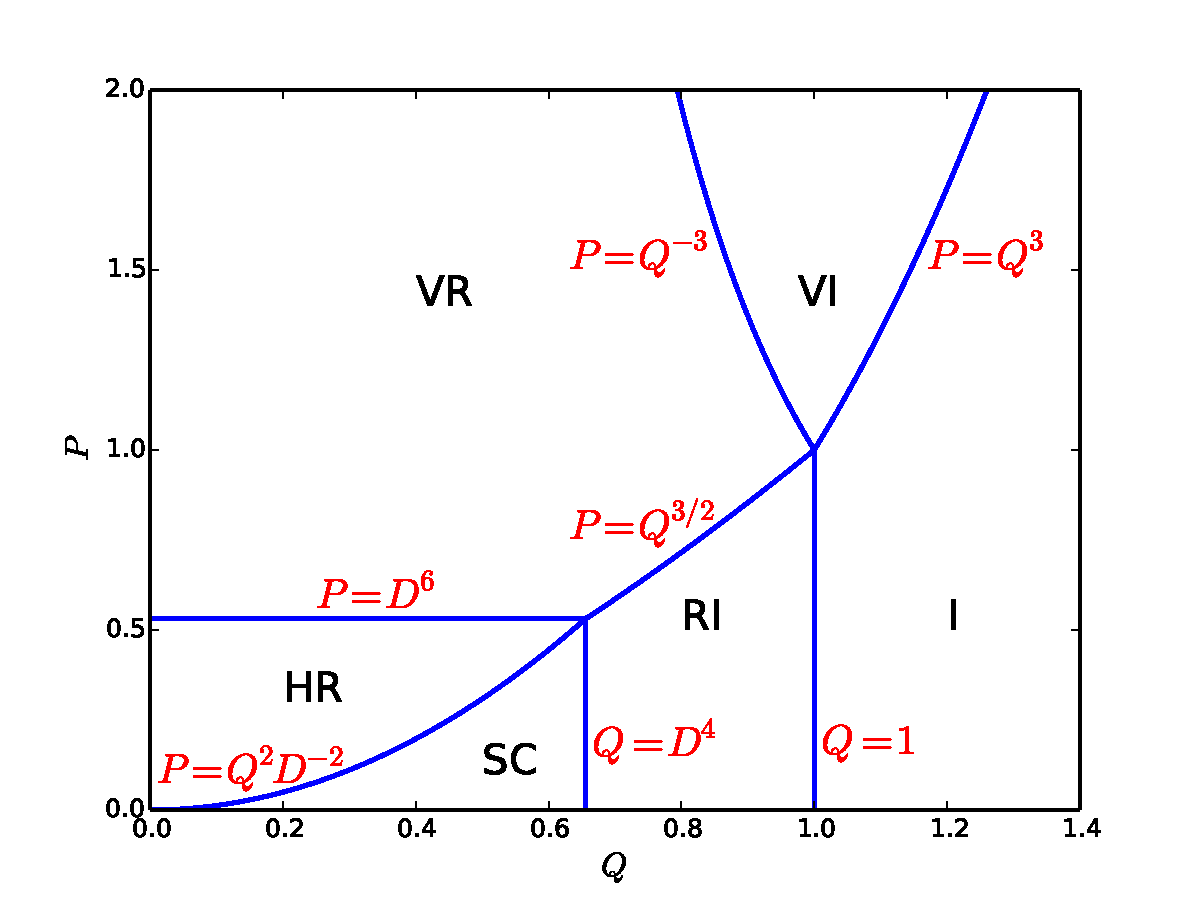
\includegraphics[width=0.9\textwidth]{RegimeI.pdf}}
\caption{Linear resonant plasma response regimes in $Q$-$P$ space for the case $D=0.9$. The various regimes are
the Hall-resisitive (HR), the semi-collisional (SC), the resistive-inertial (RI), the visco-resistive (VR), the visco-inertial
(VI), and the inertial (I).}\label{f1}
\end{figure}

Suppose that $Q\gg P\,p^2$ and $D^2\,p^2 \ll 1$. It follows that $\nu=1/2$ and
\begin{equation}
C = [-{\rm i}\,(Q-Q_E)]\,[-{\rm i}\,(Q-Q_E-Q_i)].
\end{equation}
Hence, we deduce that
\begin{equation}
\hat{\mit\Delta} = -\frac{\pi}{[-{\rm i}\,(Q-Q_E)]^{1/2}\,[-{\rm i}\,(Q-Q_E-Q_i)]^{1/2}}.
\end{equation}
This response regime is known as the {\em inertial regime}, because the layer response is dominated by
 ion inertia (Ara, et al.\ 1976; Fitzpatrick 1998). Note that the plasma response in the inertial regime is
 equivalent to that of two closely spaced Alfv\'{e}n resonances that straddle the resonant surface (Boozer 1996). 
 The characteristic layer width is $p_\ast \sim Q^{-1}$,
which implies that the regime is valid when $P\ll Q^3$, $Q\gg D$, and $Q\gg 1$. 

Suppose that $Q\ll P\,p^2$ and $D^2\,p^2 \ll 1$. It follows that $\nu=1/4$ and
\begin{equation}
C = (-{\rm i}\,[Q-Q_E-(1+\lambda_e)\,Q_e])\,P_\varphi.
\end{equation}
Hence, we deduce that
\begin{equation}
\hat{\mit\Delta} =- \frac{\pi}{2}\,\frac{{\mit\Gamma}(1/4)}{{\mit\Gamma}(3/4)}\, (-{\rm i}\,[Q-Q_E-(1+\lambda_e)\,Q_e])^{-1/4}\,P_\varphi^{-1/4}.
\end{equation}
This response regime is known as the {\em visco-inertial regime}, because the layer response is dominated by
perpendicular viscosity and ion inertia (Fitzpatrick 1998). 
 The characteristic layer width is $p_\ast \sim Q^{-1/4}\,P^{-1/4}$,
which implies that the regime is valid when $P\gg Q^3$, $P\gg D^4/Q$, and $P\gg Q^{-3}$. 

Suppose, finally, that $Q\ll P\,p^2$ and $D^2\,p^2\gg 1$. It follows that $\nu=1/2$ and
\begin{equation}
C = \frac{(-{\rm i}\,[Q-Q_E-(1+\lambda_e)\,Q_e)]\,P_\perp}{[(1+\lambda_e)+1/\tau]\,D^2}.
\end{equation}
Hence, we deduce that
\begin{equation}
\hat{\mit\Delta}= -\frac{\pi\,[(1+\lambda_e)+1/\tau]^{1/2}\,D}{(-{\rm i}\,[Q-Q_E-(1+\lambda_e)\,Q_e)])^{1/2}\,P_\perp^{1/2}}.
\end{equation}
This response regime is known as the {\em Hall-viscous regime}. The characteristic layer width is $p_\ast\sim
D\,Q^{-1/2}\,P^{-1/2}$, which implies that the regime is valid when $Q\ll D$, $P\ll D^4/Q$, and $P\gg D^2/Q^2$. 

\begin{figure}[t]
\centerline{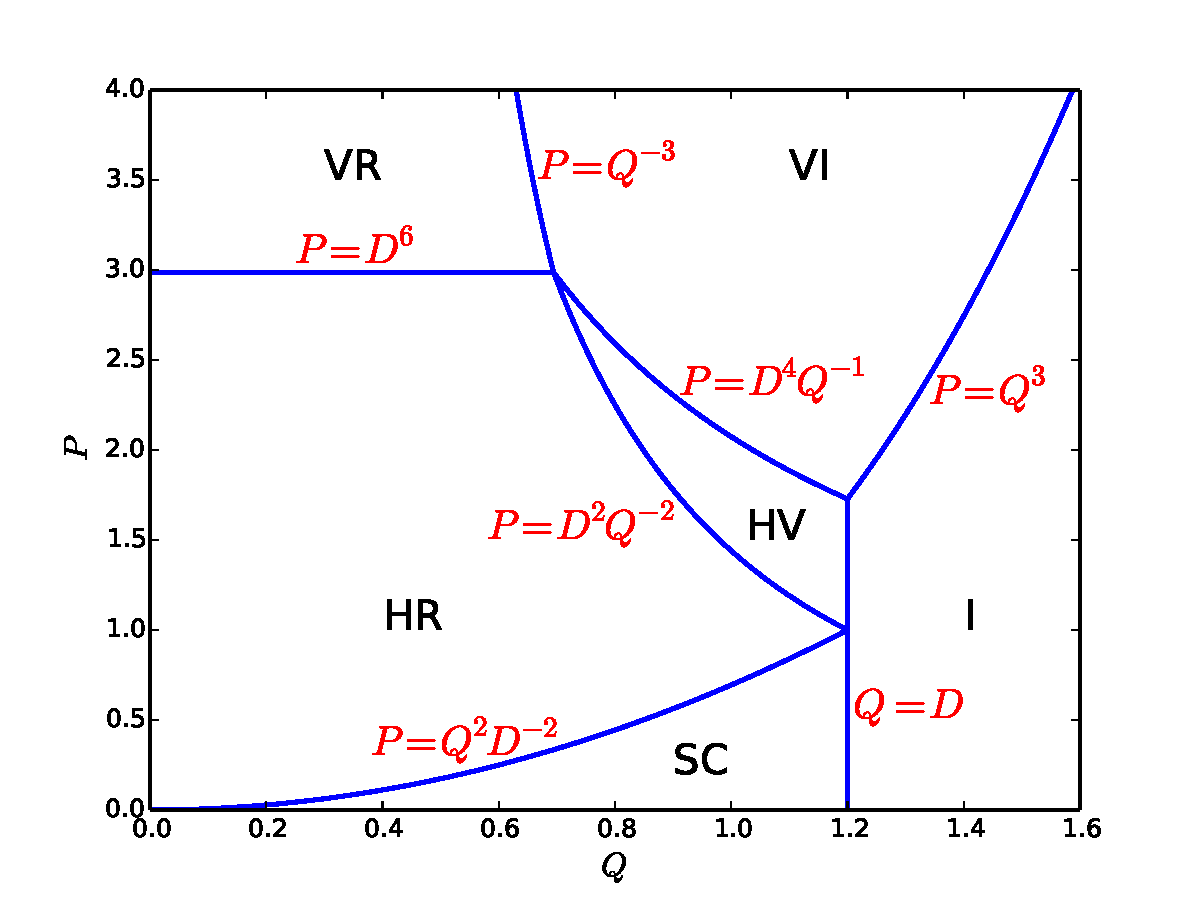
\includegraphics[width=0.9\textwidth]{RegimeII.pdf}}
\caption{Linear resonant plasma response regimes in $Q$-$P$ space for the case $D=1.2$. The various regimes are
the Hall-resisitive (HR), the semi-collisional (SC), the Hall-viscous (HV), the visco-resistive (VR), the visco-inertial
(VI), and the inertial (I).}\label{f2}
\end{figure}

\subsection{Discussion}\label{dis1}
Figures~\ref{f1} and \ref{f2} show the extents of the various different response regimes in $Q$-$P$ space for the
cases $D<1$ and $D>1$, respectively. 

Let $\hat{\delta}_\ast\sim p_\ast^{-1}$ be the normalized radial thickness of the resonant layer.  Of course, the true thickness is
$\delta = S^{-1/3}\,\hat{\delta}_\ast\,r_s$.  It follows from
Equation~(\ref{e311}) that the relative change in the perturbed helical flux, $\tilde{\psi}$, across the layer
is
\begin{equation}
\left.\frac{d\ln\tilde{\psi}}{dX}\right|_{-\hat{\delta}/2}^{+\hat{\delta}/2} = \hat{\mit\Delta}\,\,\hat{\delta}_\ast\sim \hat{\mit\Delta}\,\,p_\ast^{-1},
\end{equation}
According to the  analysis of Section~\ref{scp}, $\hat{\mit\Delta}\,p_\ast^{-1}$ takes the respective values $Q^{1/2}$, $Q\,P^{1/3}$, 
$Q^2/D^2$, and $Q\,P^{1/2}/D$ in the resistive-inertial, visco-resistive, semi-collisional, and
Hall-resistive response regimes. Moreover, it is clear from Figures~\ref{f1} and \ref{f2} that these values are all
much less than unity. In other words, it is indeed the case that $\tilde{\psi}$ does not vary substantially across a
`constant-$\psi$' resonant layer. On the other hand, according to the analysis of Section~\ref{sncp}, $\hat{\mit\Delta}\,p_\ast^{-1}\sim 1$ in the inertial,
visco-inertial, and Hall-viscous response regimes, which implies that $\tilde{\psi}$ does vary substantially
across a `nonconstant-$\psi$' layer. 

\begin{figure}[t]
\centerline{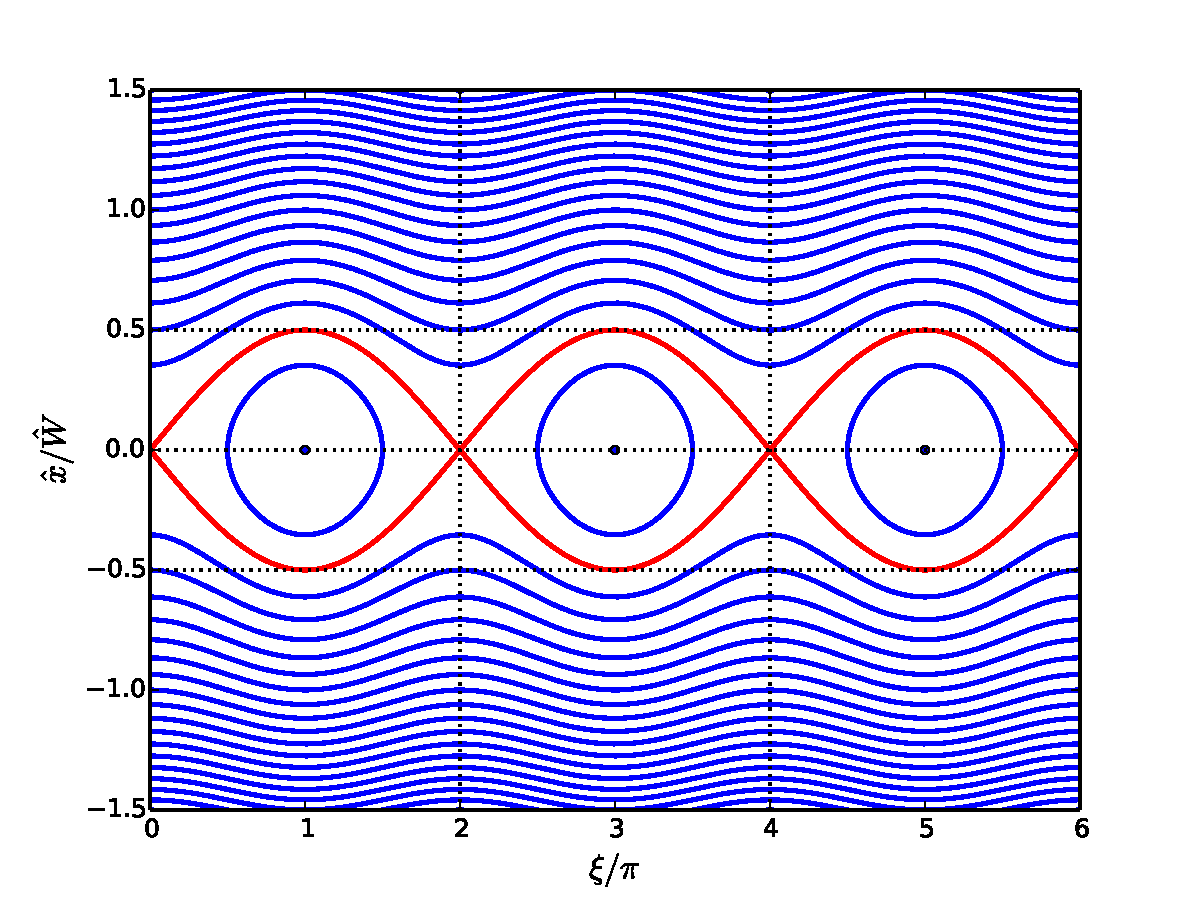
\includegraphics[width=0.9\textwidth]{Island.pdf}}
\caption{Equally-spaced contours of $\psi(\hat{x},\xi)$. The magnetic separatrix is shown in red. }\label{f2a}
\end{figure}

Suppose that the resonant layer lies in a constant-$\psi$ response regime. According to Equation~(\ref{e295}),
the perturbed magnetic flux in the layer takes the form:
\begin{equation}
\hat{\psi}(\hat{x},\zeta,t) = \frac{\hat{x}^{\,2} }{2\,\hat{L}_s}+ \tilde{\psi}\,{\rm e}^{\,{\rm i}\,(\zeta-\hat{\omega}\,\hat{t})},
\end{equation}
where $\tilde{\psi}$ is a complex constant. Of course, the physical flux is the real part of the previous expression; that is,
\begin{equation}\label{e352a}
\hat{\psi}(\hat{x},\xi)= \frac{\hat{x}^{\,2} }{2\,\hat{L}_s}+ |\tilde{\psi}|\,\cos\xi,
\end{equation}
where
\begin{equation}
\xi = \zeta +{\rm arg}(\tilde{\psi})-\hat{\omega}\,\hat{t} = m\,\theta-n\,\varphi +{\rm arg}(\tilde{\psi}) -\omega\,t.
\end{equation}
Now, it is clear from Equation~(\ref{e279}) that ${\bf B}\cdot\hat{\nabla}\hat{\psi}=0$. In other words, the contours of
$\hat{\psi}(\hat{x},\xi)$ map out the perturbed magnetic flux-surfaces in the vicinity of the resonant layer. 
Let $\hat{W} = 4\,(|\tilde{\psi}|\,\hat{L}_s)^{1/2}$. Equation~(\ref{e352a}) can be written
\begin{equation}
\frac{\psi(\hat{x},\xi)}{|\tilde{\psi}|} = 8\left(\frac{\hat{x}}{\hat{W}}\right)^2 + \cos\xi.
\end{equation}
Figure~\ref{f2a} shows the contours of $\psi(\hat{x},\xi)$ specified by the previous equation. It can be seen that the
tearing mode has reconnected magnetic field-lines to produce a {\em helical magnetic island chain}\/ centered on the resonant
surface. The chain has $m$ periods in the poloidal direction, $n$ periods in the toroidal direction, and propagates at the
helical phase velocity $\omega$. The maximum full (as opposed to half) radial width of the magnetic separatrix is 
\begin{equation}\label{e355s}
W =  \hat{W}\,r_s= 4\,(|\tilde{\psi}|\,\hat{L}_s)^{1/2}\,r_s = 4\left(\frac{q_s}{s_s}\,|\hat{\mit\Psi}_s|\right)^{1/2}R_0,
\end{equation}
where ${\mit\Psi}_s = r_s\,B_z\,\tilde{\psi}$ is the reconnected magnetic flux defined in Equation~(\ref{e99}), and
$\hat{\mit\Psi}_s= {\mit\Psi}_s/(R_0\,B_z)$. 

Finally, our four-field resonant plasma response model, (\ref{e264})--(\ref{e269}), contains many term of the general form $[\hat{\psi},\tilde{A}]$,
where $\tilde{A}(\hat{x},\zeta)$ is a perturbed quantity. According to Equation~(\ref{e352a}), such terms
can be written
\begin{equation}
[\hat{\psi},\tilde{A}] = {\rm i}\,\frac{m}{r_s}\left(\frac{\hat{x}}{\hat{L}_s}\,\tilde{A} - \tilde{\psi}\,\frac{\partial \tilde{A}}{\partial\hat{x}}\right)
\sim {\rm i}\,\frac{m}{r_s}\,\frac{\hat{\delta}}{\hat{L}_s}\,\tilde{A} - {\rm i}\,\frac{m}{r_s}\,\frac{\tilde{\psi}}{\hat{\delta}}\,\tilde{A}, 
\end{equation}
where $\delta = \hat{\delta}\,r_s$ is the width of the linear layer. Now, linear layer theory is only valid when the second
term on the extreme right side of the previous equation is negligible compared to the first (because the second term is quadratic in perturbed quantities, whereas the first is linear). In other words,
we require $\hat{\delta}^{\,2}\gg |\tilde{\psi}|\,\hat{L}_s$, which reduces to 
\begin{equation}
\delta \gg W.
\end{equation}
[See Equation~(\ref{e355s}).]
We conclude that the linear resonant response theory presented in this section is only valid when the radial width of the magnetic
island chain that develops in the vicinity of the resonant surface is {\em much less}\/ than the radial width of the linear layer. 
Given that linear layers are very narrow in conventional tokamak plasmas, this is a stringent constraint. 

\section{Linear Tearing Mode Stability}
\subsection{Introduction}
The aim of this section is to combine the analysis of Sections~\ref{cyl} and \ref{linear} to determine the linear stability
of tearing modes in tokamak plasmas. In this study, we shall assume that the wall is perfectly conducting. 

\subsection{Linear Dispersion Relation}\label{s6.2}
Let us write
\begin{equation}\label{e350}
\omega = \gamma+{\rm i}\,\omega_r,
\end{equation}
where $\gamma$ is the growth-rate of the tearing mode, whereas $\omega_r$ is the real
phase velocity of the mode in the laboratory frame. We shall assume that $|\gamma|\ll |\omega_r|$. This assumption can
easily be verified {\em a posteriori}. Asymptotic matching between the solution in the outer region and that in the
thin linear layer surrounding the resonant surface yields a linear tearing mode dispersion relation of the form
\begin{equation}\label{e352}
S^{1/3}\,\hat{\mit\Delta}(\gamma,\omega_r) = E_{ss},
\end{equation}
where use has been made of Equations~(\ref{e110}) and (\ref{e312}). Here, $E_{ss}$ is the real tearing stability index, 
whereas the complex layer matching parameter, $\hat{\mit\Delta}$, is defined in Equation~(\ref{e311}). 

In a conventional tokamak plasma [assuming that $m\sim {\cal O}(1)$], $E_{ss}\sim {\cal O}(1)$,\footnote{Note that we are neglecting $m=1$ modes, for which $|E_{ss}|\gg 1$,
because such modes are not really tearing modes
(Wesson 1978).} and $S^{1/3}\gg 1$. Hence, the previous dispersion relation can only be satisfied if $\omega_r$ takes a
value that renders $|\hat{\mit\Delta}|\ll 1$. It is clear from Equations~(\ref{ri}), (\ref{vr}), (\ref{sc}), and (\ref{hr}) that this goal
can be achieved in all of the constant-$\psi$ linear response regimes if
\begin{equation}\label{e353}
\omega_r = \omega_{\perp\,e},
\end{equation}
where
\begin{equation}\label{e354}
\omega_{\perp\,e} = \omega_E+(1+\lambda_e)\,\omega_{\ast\,e}.
\end{equation}
According to Equations~(\ref{e353}) and (\ref{e354}), the tearing mode co-rotates with the electron fluid at the resonant
 surface.\footnote{In fact, the mode 
rotates slightly faster than the electron fluid because of the influence of the thermal force, ${\bf F}_T$ [see Equation~(\ref{e43})],
which generates the additional  factor $\lambda_e$ in Equation~(\ref{e354}).}

\subsection{Determination of Linear Growth-Rates}\label{s6.3}
Reusing the analysis of Sections~\ref{s5.6} and \ref{scp}, let us again suppose that there are two layers in $p$ space (i.e., Fourier space). The
small-$p$ layer turns out to be of width $|\hat{\gamma}|^{1/2}$, where $\hat{\gamma} = S^{1/3}\,\gamma\,\tau_H$. Given that we are effectively assuming that
$|\hat{\gamma}|\ll 1$, the condition for the separation of the layer solution into two layers (i.e., that the width of the small-$p$ layer is less than that of the large-$p$ layer) is always satisfied. The large-$p$ layer is governed by the equation
\begin{equation}\label{e355}
\frac{d^{\,2} Y}{dp^2} - \frac{A(p)}{\tilde{B}(p)} \,Y =0,
\end{equation}
where 
\begin{align}
A(p) &= (1+\lambda_e)\left(\frac{\tau}{1+\tau}\right)\left(1+ \frac{\lambda_e\,\tau}{1+\tau}\right)Q_\ast^{\,2}
-{\rm i}\left(1+\frac{\lambda_e\,\tau}{1+\tau}\right)Q_\ast\,(P_\varphi+P_\perp)\,p^2\nonumber\\[0.5ex]
\phantom{=} &+ P_\varphi\,P_\perp\,p^4,\\[0.5ex]
\tilde{B}(p)&= P_\perp - {\rm i}\,(1+\lambda_e)\left(1+\frac{\lambda_e\,\tau}{1+\tau}\right)Q_\ast\,D^2 +\left(\frac{1+\tau}{\tau}\right)\left(1+\frac{\lambda_e\,\tau}{1+\tau}\right) D^2\,P_\varphi\,p^2.
\end{align}
Here, $Q_\ast = S^{1/3}\,\omega_\ast\,\tau_H$, where
\begin{equation}
\omega_\ast = -\frac{m}{r_s}\frac{1}{e\,n_0\,B_z}\left.\frac{dp}{dr}\right|_{r_s}.
\end{equation}
In the following, $\omega_\ast$ is assumed to be positive. The boundary conditions on Equation~(\ref{e355}) are
that $Y$ is bounded as $p\rightarrow\infty$, and
\begin{equation}\label{e359}
Y(p)= Y_0\left[1+\frac{\hat{\mit\Delta}\,p}{\pi\,\hat{\gamma}} + {\cal O}(p^2)\right]
\end{equation}
as $p\rightarrow 0$. 

In the various constant-$\psi$ linear response regimes considered in this section, Equation~(\ref{e355}) reduces to an equation of the form
\begin{equation}
\frac{d^{\,2} Y}{dp^2} - C\,p^m\,Y = 0,
\end{equation}
where $m$ is real and non-negative, and $C$ is a complex constant. As described in Section~\ref{s5.6}, the solution of this
equation that is bounded as $p\rightarrow \infty$ can be matched to the small-$p$ asymptotic form (\ref{e359}) to give 
\begin{equation}
\hat{\mit\Delta} = \pi\,\hat{\gamma}\,\frac{{\mit\Gamma}(1-\nu)}{{\mit\Gamma}(\nu)}\,\nu^{2\nu-1}\,C^{\,\nu},
\end{equation}
where $\nu=1/(m+2)$. The width of the large-$p$ layer in $p$ space is $C^{-\nu}$. 

As before, we shall assume that $P_\varphi\sim P_\perp \sim P$, $\lambda_e\sim{\cal O}(1)$, and $\tau\sim {\cal O}(1)$, for
the sake of simplicity. 
Suppose that $Q_\ast\gg P\,p^2$ and $P\gg Q_\ast\,D^2$. It follows that $\nu=1/2$ and
\begin{equation}
C = (1+\lambda_e)\left(\frac{\tau}{1+\tau}\right)\left(1+\frac{\lambda_e\,\tau}{1+\tau}\right)\frac{Q_\ast^{2}}{P_\perp}.
\end{equation}
Hence, 
\begin{equation}
\hat{\mit\Delta} = \pi\,\hat{\gamma}\left[ (1+\lambda_e)\left(\frac{\tau}{1+\tau}\right)\left(1+\frac{\lambda_e\,\tau}{1+\tau}\right)\right]^{1/2}\,\frac{Q_\ast}{P_\perp^{1/2}},
\end{equation}
and $p_\ast\sim P^{1/2}/Q_\ast$. This so-called {\em resistive-inertial regime}\/ is valid when $P\ll Q_\ast^{3/2}$ and
$P\gg Q_\ast\,D^2$. 
Making use of Equation~(\ref{e352}), the corresponding tearing mode growth-rate is
\begin{equation}\label{e363}
\gamma = \frac{E_{ss}}{\pi\left[ (1+\lambda_e)\left(\frac{\tau}{1+\tau}\right)\left(1+\frac{\lambda_e\,\tau}{1+\tau}\right)\right]^{1/2}\,}\,\frac{1}{\omega_\ast\,\tau_H\,\tau_R^{1/2}\,\tau_\perp^{1/2}}.
\end{equation}

Suppose that $Q_\ast \ll P\,p^2$ and $D^2\,p^2\ll 1$. 
It follows that $\nu=1/6$ and
$C = P_\varphi$. 
Hence, 
\begin{equation}
\hat{\mit\Delta} = 6^{2/3}\,\pi\,\hat{\gamma}\, \frac{{\mit\Gamma}(5/6)}{{\mit\Gamma}(1/6)}\,P_\varphi^{1/6}, 
\end{equation}
and $p_\ast\sim P^{-1/6}$. This so-called {\em visco-resistive regime}\/ is valid when $P\gg Q_\ast^{3/2}$ and
$P\gg D^6$. 
The corresponding tearing mode growth-rate is
\begin{equation}\label{e365}
\gamma = \frac{E_{ss}}{6^{2/3}\,\pi\,[{\mit\Gamma}(5/6)/{\mit\Gamma}(1/6)]}\,\frac{\tau_\varphi^{1/6}}{\tau_H^{1/3}\,\tau_R^{5/6}}.
\end{equation}

Suppose that $Q_\ast\gg P\,p^2$ and $P\ll Q_\ast\,D^2$. It follows that $\nu=1/2$ and
\begin{equation}
C = {\rm i}\left(\frac{\tau}{1+\tau}\right)\frac{Q_\ast}{D^2}.
\end{equation} 
Hence, 
\begin{equation}
\hat{\mit\Delta} = {\rm e}^{{\rm i}\,\pi/4}\,\pi\,\hat{\gamma}\left(\frac{\tau}{1+\tau}\right)^{1/2}\,\frac{Q_\ast^{1/2}}{D},
\end{equation}
and $p_\ast\sim D/Q_\ast^{1/2}$. This so-called {\em semi-collisional regime}\/ is valid when $P\ll Q_\ast^{\,2}/D^2$ and
$P\ll Q_\ast\,D^2$. 
The corresponding tearing mode growth-rate is
\begin{equation}\label{e368}
\gamma = \frac{E_{ss}}{\sqrt{2}\,\pi}\,\frac{d_s/r_s}{\omega_\ast^{1/2}\,\tau_H\,\tau_R^{1/2}}.
\end{equation}
Here, we have neglected the imaginary component of $\gamma$ because it merely gives rise to a small correction to the
propagation frequency of the mode. 

Suppose, finally, that $Q_\ast \ll P\,p^2$ and $D^2\,p^2\gg 1$. It follows that $\nu=1/4$ and
\begin{equation}
C = \frac{P_\perp\,[\tau/(1+\tau)]}{[1+\lambda_e\,\tau/(1+\tau)]\,D^2}.
\end{equation} 
Hence,
\begin{equation} 
\hat{\mit\Delta} = 2\pi\,\hat{\gamma}\,\frac{{\mit\Gamma}(3/4)}{{\mit\Gamma}(1/4)}\,\frac{[\tau/(1+\tau)]^{1/4}\,P_\perp^{1/4}}{[1+\lambda_e\,\tau/(1+\tau)]^{1/4}\,D^{1/2}},
\end{equation}
and $p_\ast \sim D^{1/2}/P^{1/4}$. This so-called {\em Hall-resistive regime}\/ is valid when $P\gg Q_\ast^2/D^2$ and
$P\ll D^6$. The corresponding tearing mode growth-rate is 
\begin{equation}\label{e371}
\gamma= \frac{E_{ss}}{2\pi\,[{\mit\Gamma}(3/4)/{\mit\Gamma}(1/4)]\,[1+\lambda_e\,\tau/(1+\tau)]^{-1/4}}\,\frac{(d_s/r_s)^{1/2}\,\tau_\perp^{1/4}}{\tau_H^{1/2}\,\tau_R^{3/4}}.
\end{equation}

\begin{figure}[t]
\centerline{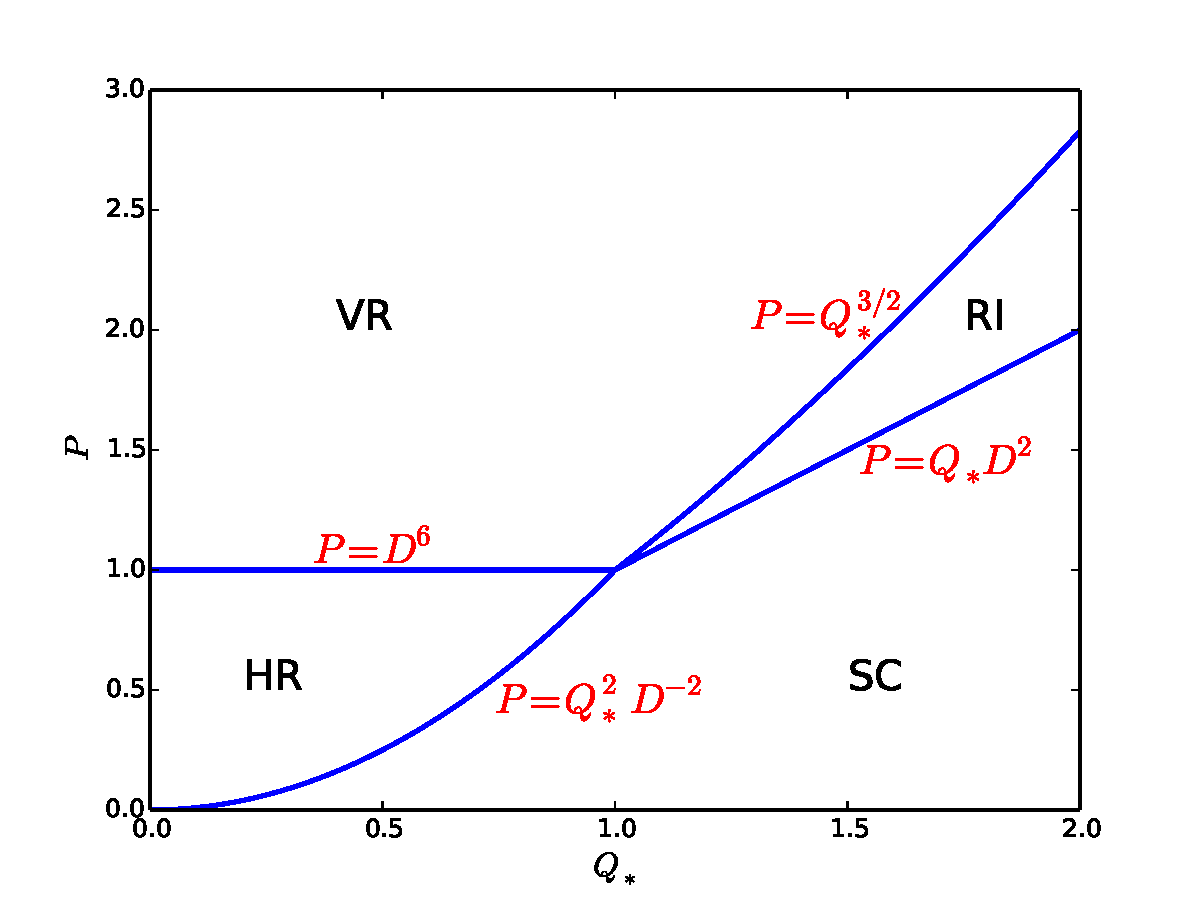
\includegraphics[width=0.9\textwidth]{RegimeIII.pdf}}
\caption{Linear tearing mode growth-rate regimes  in $Q_\ast$-$P$ space. The various regimes are
the Hall-resisitive (HR), the semi-collisional (SC),  the visco-resistive (VR), and the resistive-inertial (RI).}\label{f3}
\end{figure}

\subsection{Discussion}
According to Equations~(\ref{e350}), (\ref{e353}), (\ref{e363}), (\ref{e365}), (\ref{e368}), and (\ref{e371}), a linear tearing mode is unstable when the tearing stability index, $E_{ss}$, is positive, and is stable otherwise (Furth, et al.\ 1963).
Moreover, the perturbed magnetic field associated with the mode corotates with the electron fluid at the resonant surface (Ara, et al.\ 1978). Finally,
the mode grows on a hybrid timescale that is much greater than the hydrodynamical timescale, $\tau_H$,
but much less than the resistive evolution timescale, $\tau_R$. Note that, in all cases, the growth-rate goes to zero as
$\tau_R\rightarrow \infty$. This is not surprising because, as is clear from Equation~(\ref{e301}), the perturbed
helical magnetic flux at the resonant surface,  $\tilde{\psi}(\hat{x}=0,\zeta)$, is constrained to take the value zero
in the limit that $S\rightarrow\infty$. In other words, magnetic reconnection at the resonant surface (which corresponds to a finite
$\tilde{\psi}$ at $\hat{x}=0$) is impossible in the absence of plasma resistivity (Furth, et al.\ 1963). 

There are three main factors that
affect the growth-rate of a tearing mode in a conventional tokamak plasma. First, the strength of diamagnetic flows in the plasma, which is parameterized by the
diamagnetic frequency, $\omega_\ast$ (and by the normalized diamagnetic frequency, $Q_\ast$). Second, the  anomalous perpendicular diffusion of momentum and particles, which is parameterized by the momentum and particle confinement
timescales, $\tau_\varphi$ and $\tau_\perp$ (and by the magnetic Prandtl number, $P$). Third, finite ion sound radius effects,  which are parameterized by the modified ion sound radius, $d_s$ (and by the normalized
sound radius $D$).

 There are four tearing-mode growth-rate regimes---the resistive-inertial, the visco-resistive, the semi-collisional, and the Hall-resistive---and their extents in $Q_\ast$-$P$-$D$ space are illustrated in Figure~\ref{f3}.
Note that Figure~\ref{f3} differs somewhat from Figures~\ref{f1} and \ref{f2} because in the latter two
figures it is assumed that $|Q-Q_E-(1+\lambda_e)\,Q_e|\sim |Q-Q_E|\sim |Q-Q_E-Q_i|$ whereas
in the former figure it is assumed that $|Q-Q_E-(1+\lambda_e)\,Q_e|\ll |Q-Q_E|\sim |Q-Q_E-Q_i|$.
This refined ordering eliminates the nonconstant-$\psi$ response regimes, and significantly modifies the
resistive-inertial response regime. 

The absence of nonconstant-$\psi$ response regimes in Figure~\ref{f3}
should come as no surprise. As we saw in Section~\ref{dis1}, nonconstant-$\psi$ resonant layers
are characterized by $\hat{\mit\Delta}\sim\hat{\delta}_\ast^{-1}= S^{-1/3}\,(r_s/\delta)$, where $\delta$
is the layer thickness. Hence, according to Equation~(\ref{e352}), asymptotic matching of such a
layer to the outer solution is only possible if $|E_{ss}|\sim r_s/\delta \gg 1$ (given that resonant
layers in tokamak plasmas are invariably very thin compared to the minor radius of the plasma). However,
low-$m$ tearing modes in conventional tokamak plasmas are characterized by $|E_{ss}|\sim 1$ rather than
$|E_{ss}|\gg 1$. (As before, we are neglecting $m=1$ modes, which are characterized by
$|E_{ss}|\gg 1$, because they are not really tearing modes.)

Diamagnetic flows modify the tearing mode growth-rate in the resistive-inertial and semi-collisional
growth-rate regimes, but not in the Hall-resistive and visco-resistive regimes. Anomalous perpendicular
transport modifies the growth-rate in all regimes except the semi-collisional regime. Finally, finite ion sound radius 
effects modify the growth-rate in the Hall-resistive and semi-collisional regimes, but not in the other two
regimes. 

Increasing  the diamagnetic flow strength decreases the tearing mode growth-rate such that it
eventually scales as $\omega_\ast^{-1/2}$. Increasing the anomalous perpendicular transport increases the
growth-rate such that it  eventually scales as $P_\varphi^{1/6}$. Increasing the ion sound radius 
increases the tearing mode growth-rate, but the increase eventually saturates (i.e., the
growth-rate ends up scaling as $d_s^{\,0}$). 

Finally, it is clear from Equation~(\ref{e352}) that the layer solution can only be matched to the
outer solution when $\omega_r$ takes a value that renders $|\hat{\mit\Delta}|\ll 1$. We have seen that this
is possible in all constant-$\psi$ response regimes when $\omega_r= \omega_E+(1+\lambda_e)\,\omega_{\ast\,e}$
(i.e., when the tearing perturbation corotates with the electron fluid at the resonant surface.) However, Equation~(\ref{ri})
seems to suggest that in the resistive-inertial regime it might be possible to successfully match the
layer solution to the outer solution when $\omega_r=\omega_E$ (i.e., $Q=Q_E$), or when 
$\omega_r=\omega_E+\omega_{\ast\,i}$
(i.e., $Q=Q_E+Q_i$),
giving tearing mode perturbations that corotate with the MHD fluid and the ion fluid, respectively, at the resonant
surface. In fact, we can see that this is not the case, because if we set $\omega_r=\omega_E$ or $\omega_r=\omega_E+\omega_{\ast\,i}$  then Equation~(\ref{e329}) does not lead to a layer solution characterized by  $|\hat{\mit\Delta}|\ll 1$, 
as a consequence of finite anomalous perpendicular transport. Likewise, Equation~(\ref{sc}) seems to suggest that in the semi-collisional response regime it might be possible to successfully match the
layer solution to the outer solution when $\omega_r=\omega_E$, giving rise to a tearing perturbation that corotates with the MHD fluid at the resonant surface.  In fact, this possibility is also ruled out by finite anomalous
perpendicular transport. 

\section{Error-Field Penetration in Tokamak Plasmas}
\subsection{Introduction}
Tokamak plasmas are invariably subject to small amplitude, static, resonant magnetic pert\-urbations---known as
{\em error-fields}---which are primarily generated by field-coil misalignments and uncompensated coil feeds. 
Error-fields can drive magnetic reconnection, resulting in the formation of {\em locked}\/ (i.e., non-rotating in the laboratory
frame) magnetic island chains, in intrinsically tearing-stable plasmas. Low-density, ohmically-heated tokamak plasmas
containing locked magnetic island chains often terminate in sudden violent events known as {\em disruptions}\/ (Wesson, et al.\ 1989; Wesson 2011) (usually triggered when the
external heating is turned on). Fortunately, error-field driven magnetic reconnection is strongly
suppressed by the naturally occurring rotation of ohmic plasmas. However, when the error-field amplitude rises
above a certain critical amplitude, the rotation at the resonant surface is suddenly arrested, and error-field driven reconnection proceeds
unhindered. This phenomenon is known as {\em error-field penetration}\/ (Fitzpatrick 1993; Fitzpatrick 1998). The scenario
just outlined has been observed in a number of tokamak experiments (Scoville, et al.\ 1991; Hender, et al.\ 1992; Fishpool
\& Haynes 1994; Wolfe, et al.\ 2005; Wolf, et al.\ 2005; Howell, Hender, \& Cunningham 2007; Menard, et al.\ 2010; Wang, et al.\ 2014; Wang, et al.\ 2018).

In this section, we shall calculate the critical error-field amplitude required to trigger penetration on the assumption that,
prior to penetration, the rotational suppression of error-field driven magnetic reconnection is sufficiently strong that
the resonant plasma response is governed by linear layer physics (Fitzpatrick 1993; Fitzpatrick 1998; Cole \& Fitzpatrick 2006).

\subsection{Asymptotic Matching}
It is convenient to parametrize the error-field in terms of the static current, $I_c$, that must be run through the magnetic
field-coil introduced in Section~\ref{sfc} in order to generate it. Setting $d/dt=0$ in Equations~(\ref{e202}) and (\ref{e203}),
we get
\begin{equation}\label{e400}
{\mit\Delta\hat{\Psi}}_s = {\mit\Delta}_{nw}\,\hat{\mit\Psi}_s+\tilde{I}_c,
\end{equation}
where
\begin{equation}
{\mit\Delta}_{nw} = {\mit\Delta}_{pw} + \frac{E_{sw}^{\,2}}{(-\tilde{E}_{ww})}
\end{equation}
is the (real) tearing stability index in the absence of a wall, ${\mit\Delta}_{pw}= E_{ss}$ is the
(real) tearing stability index in the presence of a perfectly conducting wall at $r=r_w$, and
\begin{equation}
\tilde{I}_c =\left(\frac{{\mit\Delta}_{nw} - {\mit\Delta}_{pw}}{E_{sw}}\right)\left(
\frac{r_w}{r_c}\right)^m\left(\frac{\mu_0\,I_c}{R_0\,B_z}\right).
\end{equation}
Here, the plasma-wall coupling parameter, $E_{sw}>0$, is defined in Section~\ref{resistive}. We expect $0>{\mit\Delta}_{nw}>
{\mit\Delta}_{pw}$ because the plasma is assumed to be tearing stable, and $\tilde{E}_{ww}<0$. 

In the resonant layer, Equation~(\ref{e312}) yields
\begin{equation}\label{e383}
{\mit\Delta\hat{\Psi}}_s = {\mit\Delta}\,\,\hat{\mit\Psi}_s,
\end{equation}
where ${\mit\Delta} = S^{1/3}\,\hat{\mit\Delta}$, and the complex layer matching parameter, $\hat{\mit\Delta}$, is defined in 
Equation~(\ref{e312}). 
Hence, asymptotic matching between the inner and the outer regions yields
\begin{equation}\label{e384}
\hat{\mit\Psi}_s = \frac{\tilde{I}}{(-{\mit\Delta}_{nw}) + {\mit\Delta}},
\end{equation}
where use has been made of Equations~(\ref{e400}) and (\ref{e383}). 
The previous equation specifies the (normalized) reconnected magnetic flux, $\hat{\mit\Psi}_s$, driven at the resonant surface by the (normalized) 
error-field coil current, $\tilde{I}_c$. The complex layer parameter, ${\mit\Delta}$, specifies the strength of a shielding current
that is induced in the resonant layer, and acts to prevent driven magnetic reconnection. 

\subsection{Resonant Layer Response}
Generally speaking, in an ohmically-heated tokamak, we do not expect the plasma flow at the resonant surface to be sufficiently
large to cause a breakdown of the constant-$\psi$ approximation. We also expect $P_\varphi, P_\perp \gg 1$. In other
words, we expect the resistive evolution timescale to significantly exceed both the momentum and energy/particle
confinement timescales (which it generally does by, at least, a factor of 10). Hence, consulting Figures~\ref{f1} and \ref{f2},
we can see that the appropriate linear resonant response regime is either the visco-resistive regime or the Hall-resistive
regime. 

According to the analysis of Section~\ref{scp}, and making use of the fact that $\omega=Q=0$ for a static perturbation, 
in the visco-resistive response regime we have
\begin{equation}
{\mit\Delta}_{\rm VR} = {\rm i}\,\tau_{\rm VR}\,(\omega_{\perp\,e}+{\mit\Delta}\omega_E),
\end{equation}
where $\tau_{\rm VR} = \tau_R\,\hat{\delta}_{\rm VR}$, and
\begin{equation}
\hat{\delta}_{\rm VR} = \frac{6^{2/3}\,\pi\,{\mit\Gamma}(5/6)}{{\mit\Gamma}(1/6)}\,\frac{\tau_H^{1/3}}{\tau_R^{1/6}\,\tau_\varphi^{1/6}}
\end{equation}
is the visco-resistive layer width (normalized to $r_s$). Here, $\omega_{\perp\,e}$ is defined in Equation~(\ref{e354}), and
${\mit\Delta}\omega_E$ is the modification to the ${\bf E}\times{\bf B}$ frequency generated at the resonant surface by
the electromagnetic torques that develop there in response to the error-field. Likewise, in the
Hall-resistive regime we have
\begin{equation}
{\mit\Delta}_{\rm HR} = {\rm i}\,\tau_{\rm HR}\,(\omega_{\perp\,e}+{\mit\Delta}\omega_E),
\end{equation}
where $\tau_{\rm HR} = \tau_R\,\hat{\delta}_{\rm HR}$, and
\begin{equation}
\hat{\delta}_{\rm HR} = \frac{2\pi\,{\mit\Gamma}(3/4)}{{\mit\Gamma}(1/4)\,[1+\lambda_e\,\tau/(1+\tau)]^{1/4}}\,
\frac{\tau_H^{1/2}}{(d_s/r_s)^{1/2}\,\tau_R^{1/4}\,\tau_\perp^{1/4}}
\end{equation}
is the Hall-resistive layer width (normalized to $r_s$).

We can combine the previous two results to give the composite layer response equation
\begin{equation}\label{e389}
{\mit\Delta} = {\rm i}\,\tau_s\,(\omega_{s\,0}+ {\mit\Delta}\omega_E),
\end{equation}
where $\tau_s=\tau_R\,\hat{\delta}$, 
\begin{equation}
\hat{\delta} = \frac{\hat{\delta}_{\rm VR}\,\hat{\delta}_{\rm HR}}{\hat{\delta}_{\rm VR} + \hat{\delta}_{\rm HR}},
\end{equation}
and 
\begin{equation}
\omega_{s\,0}= \omega_{\perp\,e}.
\end{equation} 

It can be seen, by comparison with the analysis of Section~\ref{tauw}, that the resonant layer responds to the error-field
perturbation in an analogous manner to a thin, rigid, resistive wall whose resistivity matches that of the plasma at the
resonant surface, and whose radial thickness is $\delta=r_s\,\hat{\delta}$. Note, however, that the effective wall corotates with the
electron fluid at the resonant surface. Moreover, it is the rotation of the effective wall that generates the shielding current. 

Incidentally, the reason that a shielding current only develops in the vicinity of the resonant surface is that the plasma is
not a rigid body. Under normal circumstances, the plasma responds to the error-field by displacing radially in such a
manner as to eliminate the shielding current. The requisite displacement is (Freidberg 1987)
\begin{equation}
\xi_r(r,\zeta) = \frac{\tilde{\psi}(r,\zeta)}{B_\theta(r)\,[1-q(r)/q_s]}.
\end{equation}
However, this displacement becomes infinite at the resonant surface, where $q(r)=q_s$, which explains why a shielding
current is only excited in the immediate vicinity of this surface. 

Equations~(\ref{e384}) and (\ref{e389}) yield
\begin{equation}\label{e392}
\hat{\mit\Psi}_s=\frac{\tilde{I}_c}{(-{\mit\Delta}_{nw})+ {\rm i}\,\tau_s\,(\omega_{s\,0}+ {\mit\Delta}\omega_E)}.
\end{equation}
Now, in a conventional ohmically-heated tokamak plasma, $\tau_s\,\omega_{s\,0}\gg (-{\mit\Delta}_{nw})$. Consequently, the
shielding current that develops at the resonant surface, in response to the local plasma rotation, is strong enough to largely
suppress error-field-driven magnetic reconnection [i.e., $|\hat{\mit\Psi}_s|\ll |\tilde{I}_c|/(-{\mit\Delta}_{nw})$]. However, the shielding current also gives rise to a localized electromagnetic
torque at the resonant surface (see Section~\ref{storque}) that acts to slow the plasma rotation. 

\subsection{Torque Balance}\label{stb}
According to Equations~(\ref{e200}) and (\ref{e201}),
\begin{equation}\label{e393}
{\mit\Delta}\omega_E = ({\bf k}\cdot{\mit\Delta}{\bf V}_i)_{r=r_s} = -\sum_{p=1,\infty}(\alpha_p+ \beta_p).
\end{equation}
In other words, the shift in the ${\bf E}\times {\bf B}$ velocity at the resonant surface, in response to the electromagnetic
torques that develop there, is mirrored by an equal  shift in the ion fluid velocity. This is the
essence of the no-slip constraint discussed in Section~\ref{sns}. The no-slip constaint follows from Equations~(\ref{e217}) and (\ref{e219})
because the torques do not modify the diamagnetic velocity at the resonant surface. 

Making use of Equations~(\ref{e193}), (\ref{e194}), (\ref{e205}) and (\ref{e206}) (with $d/dt=0$), (\ref{e383}), (\ref{e389}), (\ref{e392}),
and (\ref{e393}), we arrive at the following torque balance equation (Fitzpatrick 1993; Fitzpatrick 1998):
\begin{equation}\label{e394}
T_{\rm VS}(v)= T_{\rm EM}(v),
\end{equation}
where 
\begin{align}
v&=\frac{\omega_{s\,0}+{\mit\Delta}\omega_E}{\omega_{s\,0}},\\[0.5ex]
T_{\rm VS}(v) &= 1- v,\\[0.5ex]
T_{\rm EM}(v) &= \frac{1}{4}\,\frac{v}{\zeta_s^{\,2}+v^2}
\left(\frac{|\tilde{I}_c|}{\tilde{I}_{c\,{\rm crit}}}\right)^2,\\[0.5ex]
\zeta_s &= \frac{(-{\mit\Delta}_{nw})}{\tau_s\,\omega_{s\,0}}\ll 1,\\[0.5ex]
\tilde{I}_{c\,{\rm crit}}&= (\epsilon_s\,s_s)\,(\omega_{s\,0}\,\tau_H)\left/
\left[\frac{q_s}{\epsilon_s}\left(\frac{\sqrt{\tau_\varphi\,\tau_{i\,s}/\mu_{00\,s}^i}}{\tau_s}\right)+2\left(\frac{\tau_\varphi}{\tau_s}\right) \ln\!\left(\frac{a}{r_s}\right)\right]^{1/2}\right..\label{e420}
\end{align}
Here, use has been made of the identities
\begin{align}
\lim_{\epsilon\rightarrow 0}\sum_{p=1,\infty} \frac{\sqrt{\epsilon}\,[J_1(j_{1\,p}\,x)]^{2}}{[J_2(j_{1\,p})]^2\,(1+\epsilon\,j_{1\,p}^2)}
&=\frac{1}{4\,x},\\[0.5ex]
\sum_{p=1,\infty} \frac{[J_0(j_{0\,p}\,x)]^2}{[J_1(j_{0\,p}\,x)]^2\,j_{0\,p}^{\,2}} =\frac{1}{2}\,\ln\!\left(\frac{1}{x}\right).
\end{align}
We have also written 
\begin{equation}
\frac{1}{\tau_{\theta\,s}} = \left(\frac{q_s}{\epsilon_s}\right)^2\,\left(\frac{\mu_{00\,s}^i}{\tau_{i\,s}}\right),
\end{equation}
 where
 \begin{align}
\tau_{i\,s}&= \tau_i(r_s),\\[0.5ex]
 \mu_{00\,s}^i&=\mu_{00}^i(r_s), 
 \end{align}
 and $\mu_{00}^i(r)$ is a dimensionless neoclassical viscosity coefficient defined in Fitzpatrick \& Nelson 2020. Furthermore,
 we have assumed that $\tau_{i\,s}/(\tau_\varphi\,\mu_{00\,s}^i)\ll (q_s/\epsilon_s)^2$ (this
turns out to be  
a very good approximation because the ion collision time, $\tau_{i\,s}$, is much less than the momentum confinement
time, $\tau_\varphi$, in conventional tokamak plasmas).  

\begin{figure}[t]
\centerline{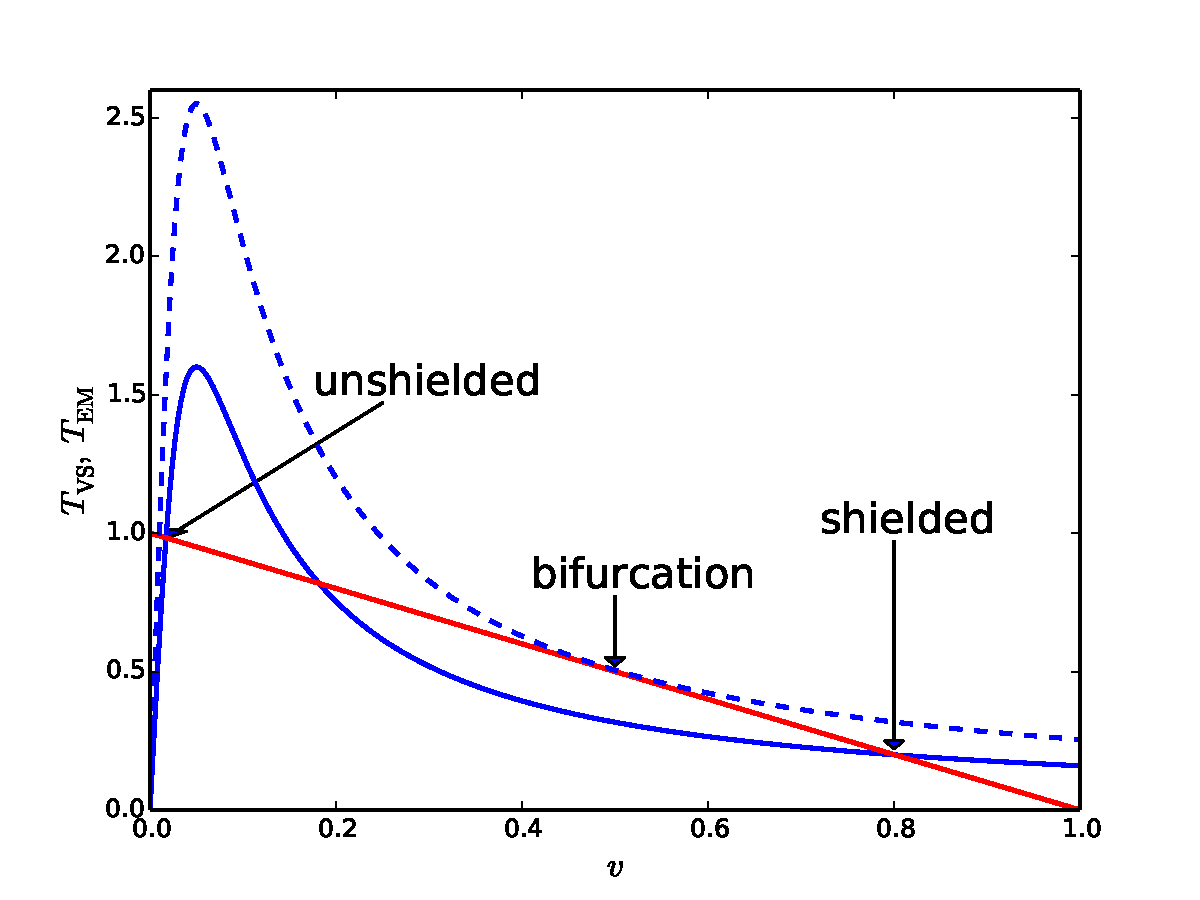
\includegraphics[width=0.9\textwidth]{Torque.pdf}}
\caption{Torque balance. The red curve shows the normalized viscous restoring torque, $T_{\rm VS}(v)$. The
solid and dashed blue curves show the normalized electromagnetic locking torque, $T_{\rm EM}(v)$,
evaluated with $\zeta_s=0.05$, and
 $|\tilde{I}_c|/\tilde{I}_{c\,{\rm crit}}=0.8$ and $1.0$, respectively. }\label{f5}
\end{figure}

In Equation~(\ref{e394}), the dimensionless
parameter $v$ takes the value unity when the plasma (i.e., electron fluid) rotation at the resonant surface is unmodified by
the electromagnetic locking torque, and zero when the electromagnetic locking torque has reduced the rotation to zero. The electromagnetic torque itself
is represented  by the function $T_{\rm EM}(v)$, whereas the viscous restoring toque that acts to oppose changes in the plasma rotation is represented
by the function $T_{\rm VS}(v)$. It can be seen from Figure~\ref{f5} that, while the viscous restoring torque varies linearly with $v$,
the electromagnetic locking torque varies with $v$ in a nonmonotonic manner. The electromagnetic torque is
zero when $v=0$, because there is no plasma rotation to induce a shielding current. As $v$ increases from zero, the
torque initially increases linearly with $v$. However, the shielding current eventually becomes strong enough to expel
the reconnected magnetic flux from the resonant layer. Consequently, because the torque
is proportional to the product of the shielding current and the reconnected flux, the torque peaks, and ends up falling off as $1/v$ 
with increasing $v$ (Gimbett \& Peckover 1979; Fitzpatrick 1993). 

The solutions of the torque balance equation (\ref{e394}) correspond to the crossing points of the viscous and electromagnetic torque
curves. As is clear from Figure~\ref{f5}, if the normalized magnitude of the error-field coil current, $|\tilde{I}_c|$, lies below
the critical value $\tilde{I}_{c\,{\rm crit}}$ then there are three crossing points. However, the intermediate crossing point corresponds to
a dynamically unstable equilibrium. Hence, we deduce that there are two physical solution branches of the torque
balance equation. The large-$v$ solution branch corresponds to  so-called {\em shielded}\/ solutions in which the plasma
rotation at the resonant surface is large enough to strongly suppress driven magnetic reconnection. The small-$v$
solution branch corresponds to so-called {\em unshielded}\/ solutions  in which the plasma rotation at the resonant surface is
too weak to suppress driven magnetic reconnection. 
On the shielded solution branch, Equation~(\ref{e394}) possesses the approximate solution
\begin{equation}
v \simeq \frac{1}{2}\left(1-\left[1-\left(\frac{|\tilde{I}_c|}{\tilde{I}_{c\,{\rm crit}}}\right)^2\right]^{1/2}.
\right)
\end{equation}
It can be seen that as the error-field coil current increases  the plasma rotation at the resonant surface decreases. However, when
$|\tilde{I}_c|$ attains the critical value $\tilde{I}_{c\,{\rm crit}}$, and the rotation is reduced to half of its
original value, the shielded solution branch ceases to exist, and there is a bifurcation to the unshielded solution branch (Fitzpatrick 1993;
Fitzpatrick 1998). (See Figure~\ref{f5}.)
The bifurcation is associated with a sudden decrease in the plasma rotation at the resonant surface, and a sudden
increase in the driven reconnected magnetic flux, and is identified with the error-field penetration phenomenon observed in tokamak
experiments. As is clear from Equation~(\ref{e420}), the critical error-field coil current needed to trigger error-field
penetration increases linearly with the unperturbed plasma rotation at the resonant surface, which is parameterized by $\omega_{s\,0}$. 
Once error-field penetration has occurred, the magnitude of the error-field coil current must be reduced to a value
that is substantially less than $\tilde{I}_{c\,{\rm crit}}$ in order to trigger a reverse bifurcation to the unshielded solution branch (Fitzpatrick 1998). 

Finally, the criterion for the validity of the theory presented in this section is that the width of the magnetic island
chain driven at the resonant surface, just prior to mode penetration, is much less than the linear layer width (so that the resonant
plasma response is governed by linear physics). This is the case provided that (Fitzpatrick 1998)
\begin{equation}
\hat{\delta}\gg 4\,S^{-2/5}\left(\frac{q_s}{\epsilon_s}\right)^{2/5}\left[\frac{q_s}{\epsilon_s}\left(\frac{\sqrt{\tau_\varphi\,\tau_{i\,s}/\mu_{00\,s}^i}}{\tau_R}\right)+2\left(\frac{\tau_\varphi}{\tau_R}\right) \ln\!\left(\frac{a}{r_s}\right)\right]^{-1/5}.
\end{equation}

\subsection{Scaling Analysis}
The aim of this section is to use the previous analysis to predict the scaling of the error-field penetration
threshold with the standard dimensionless scaling parameters (Connor \& Taylor 1977)
\begin{align}
\rho_\ast &= \frac{T_0^{1/2}\,m_i^{1/2}}{e\,B_z\,L_s},\label{e428}\\[0.5ex]
\nu_\ast &= \frac{L_s\,n_0\,e^2\,\eta_\parallel(r_s)}{m_e^{1/2}\,T_0^{1/2}},\\[0.5ex]
\beta&=\frac{\mu_0\,n_0\,T_0}{B_z^{\,2}},\label{e430}
\end{align}
where $T_0=p_0/n_0$. In the following, for the sake of simplicity, we
shall assume that $T_i=T_e=T_0$, $\omega_{s\,0}=\omega_\ast$, and $-(d\ln p/dr)_{r_s} = 1/r_s$. We shall also neglect ${\cal O}(1)$
constants such as $s_s$, $\eta_e$, $\eta_i$, $\lambda_e$, $\tau$, $\pi$, $\ln(r_s/a)$, et cetera.

 Now, in an ohmically-heated tokamak
plasma, the energy confinement timescale, $\tau_E$, satisfies the constraint
\begin{equation}
\frac{n_0\,T_0}{\tau_E} = \eta_\parallel(r_s)\left(\frac{B_z}{\mu_0\,L_s}\right)^2,
\end{equation}
which is obtained by equating the energy loss rate to the ohmic heating rate. Let us assume that the momentum confinement
time, $\tau_\varphi$, and the particle/energy confinement time, $\tau_\perp$, are both equal to $\tau_E$, as is generally
(approximately) the case in ohmically-heated tokamak plasmas (ITER Physics Basis Editors 1999). 

It is easily demonstrated that
\begin{align}
\omega_{s\,0}\,\tau_H&\simeq \left(\frac{q_s}{\epsilon_s}\right)^2\rho_\ast\,\beta^{\,1/2},\\[0.5ex]
\frac{\tau_H}{\tau_R}&\simeq \left(\frac{q_s}{\epsilon_s}\right)^2\left(\frac{m_e}{m_i}\right)^{1/2}\rho_\ast^{\,2}\,\nu_\ast\,\beta^{-1/2},\\[0.5ex]
\frac{\tau_\varphi}{\tau_R} = \frac{\tau_\perp}{\tau_R} &\simeq \left(\frac{q_s}{\epsilon_s}\right)^2\beta,\\[0.5ex]
\frac{\tau_{i\,s}}{\tau_R} &\simeq  \left(\frac{q_s}{\epsilon_s}\right)^2\left(\frac{m_e}{m_i}\right)^{1/2}\rho_\ast^{\,2}\,\beta^{-1},\\[0.5ex]
\frac{d_s}{r_s} &\simeq \left(\frac{q_s}{\epsilon_s}\right)\rho_\ast.
\end{align} 
Hence, we deduce that 
\begin{align}
\hat{\delta}_{\rm VR} = \left(\frac{\tau_{\rm VR}}{\tau_R}\right) \simeq\left(\frac{\tau_H}{\tau_R}\right)^{1/3}\left(\frac{\tau_R}{\tau_\varphi}\right)^{1/6}&\simeq \left(\frac{q_s}{\epsilon_s}\right)^{1/3}\left(\frac{m_e}{m_i}\right)^{1/6}\rho_\ast^{\,2/3}\,\nu_\ast^{\,1/3}\,\beta^{-1/3},\\[0.5ex]
\hat{\delta}_{\rm HR} = \left(\frac{\tau_{\rm HR}}{\tau_R}\right) \simeq \left(\frac{\tau_H}{\tau_R}\right)^{1/2}\left(\frac{\tau_R}{\tau_\perp}\right)^{1/4}\left(\frac{r_s}{d_s}\right)^{1/2}&\simeq \left(\frac{m_e}{m_i}\right)^{1/4}\rho_\ast^{\,1/2}\,\nu_\ast^{\,1/2}\,\beta^{-1/2},\\[0.5ex]
\frac{\sqrt{\tau_\varphi\, \tau_{i\,s}/\mu_{00\,s}^i}}{\tau_R}&\simeq \left(\frac{q_s}{r_s}\right)^2\left(\frac{m_e}{m_i}\right)^{1/4}\,\rho_\ast.
\end{align}
Here, we have treated $\mu_{00\,s}^i$ as an ignorable ${\cal O}(1)$ constant that is independent of $\rho_\ast$, $\nu_\ast$, and
$\beta$ [as is indeed the case provided that the plasma at the resonant surface lies in the banana collisionality regime (Hirshman \& Sigmar 1981)]. 

\begin{figure}[t]
\centerline{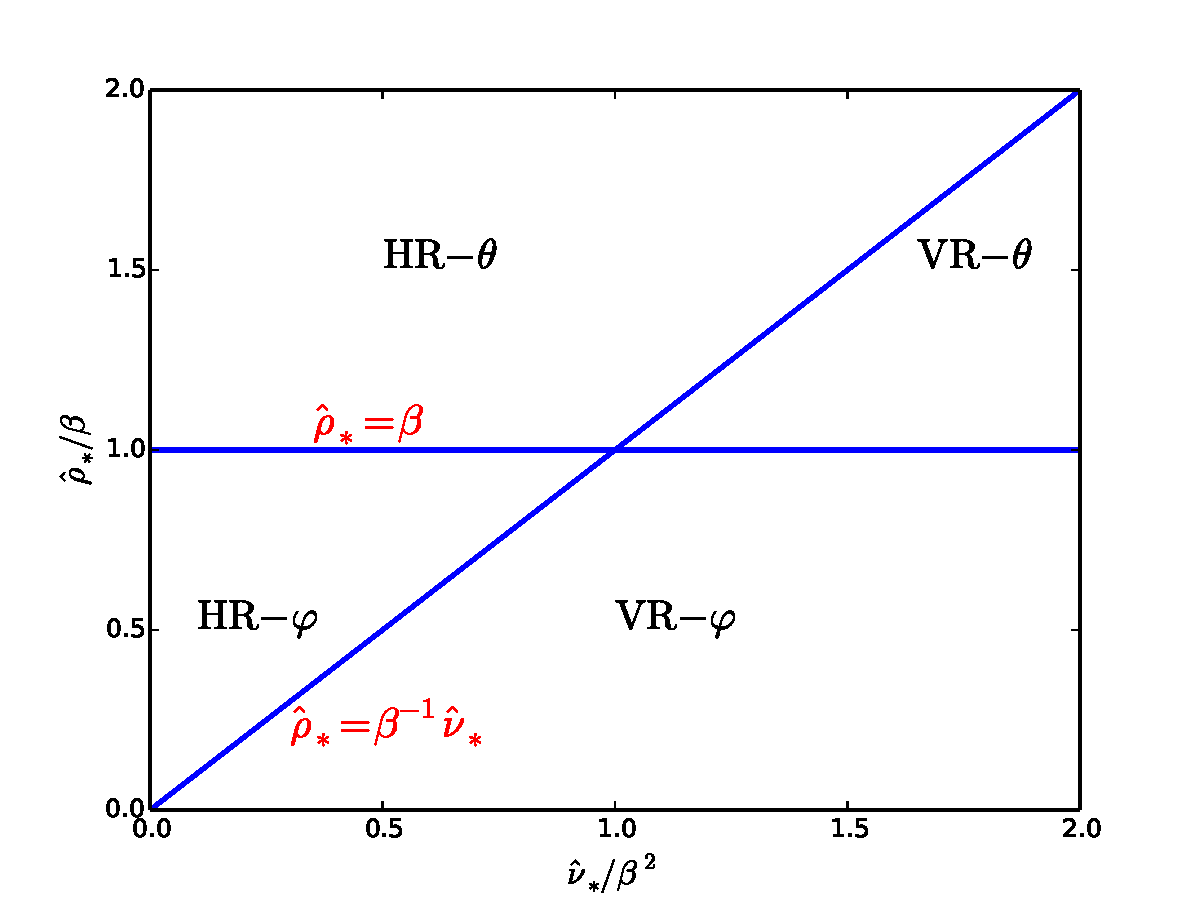
\includegraphics[width=0.9\textwidth]{Scaling.pdf}}
\caption{Error-field penetration regimes in $\hat{\nu}_\ast$-$\hat{\rho}_\ast$ space. The various regimes are the
visco-resistive-toroidal (${\rm VR}$-$\varphi$), the visco-resistive-poloidal (${\rm VR}$-$\theta$), the Hall-resistive-poloidal (${\rm HR}$-$\theta$), and the  Hall-resistive-toroidal (${\rm HR}$-$\varphi$). }\label{f6}
\end{figure}

There are four error-field penetration regimes depending on whether the plasma response in the resonant layer is
in the visco-resistive or the Hall-resistive regime, and depending on whether the change in the ion rotation at the resonant surface, induced by the electromagnetic locking torque,  is
predominately toroidal or poloidal in nature. The plasma response in the resonant layer is in the
visco-resisitive, rather than the Hall resistive, regime when $\tau_{\rm VR}<\tau_{\rm HR}$, or
\begin{equation}
\rho_\ast < \left(\frac{\epsilon_s}{q_s}\right)^2\left(\frac{m_e}{m_i}\right)^{1/2}\nu_\ast\,\beta^{-1},
\end{equation}
and vice versa. The change in the ion rotation at the resonant surface is predominately toroidal, rather than poloidal, when
\begin{equation}
\rho_\ast < \left(\frac{\epsilon_s}{q_s}\right)\left(\frac{m_i}{m_e}\right)^{1/4}\beta,
\end{equation}
and vice vera. 

Let us define 
\begin{align}
\hat{\rho}_\ast&= \left(\frac{q_s}{\epsilon_s}\right)\left(\frac{m_e}{m_i}\right)^{1/4}\rho_\ast,\\[0.5ex]
\hat{\nu}_\ast&=\left(\frac{\epsilon_s}{q_s}\right)\left(\frac{m_e}{m_i}\right)^{3/4}\nu_\ast.
\end{align}
As is illustrated in Figure~\ref{f6}, the {\em visco-resistive-toroidal regime}\/ (i.e., a visco-resistive layer response
combined with a predominately toroidal change in the ion rotation) corresponds to $\hat{\rho}_\ast < \beta^{-1}\,\nu_\ast$ 
and $\hat{\rho}_\ast <\beta$, the {\em visco-resisitive-poloidal regime}\/ corresponds to 
 $\hat{\rho}_\ast<\beta^{-1}\,\nu_\ast$ and $\hat{\rho}_\ast > \beta$, the {\em Hall-resisitive-poloidal regime}\/ corresponds to  
 $\hat{\rho}_\ast>\beta^{-1}\,\nu_\ast$ and $\hat{\rho}_\ast > \beta$, and the {\em Hall-resistive-toroidal regime}\/ corresponds to   
 $\hat{\rho}_\ast>\beta^{-1}\,\nu_\ast$ and $\hat{\rho}_\ast < \beta$.
It can be seen that higher/lower plasma collisionality (i.e., $\nu_\ast$) favors the visco-resistive/Hall-resistive response regime, whereas a
larger/smaller ion sound radius (i.e., $\rho_\ast$) favors poloidal/toroidal changes in the ion rotation. Finally, higher/lower plasma
pressure (i.e., $\beta$) 
favors the Hall-resistive/visco-resistive response regime and toroidal/poloidal changes in the ion rotation. 

In the visco-resistive-toroidal response regime, the critical vacuum (i.e., in the absence of shielding currents) radial magnetic
field at the resonant surface required to
trigger error-field penetration is
\begin{equation}\label{e444}
\left(\frac{b_{r}}{B_z}\right)_{{\rm VR}-\varphi} \simeq \epsilon_s^{-1}\tilde{I}_{c\,{\rm crit}}\simeq \left(\frac{q_s}{\epsilon_s}\right)^{7/6}\left(\frac{m_e}{m_i}\right)^{1/12}
\rho_\ast^{\,4/3}\,\nu_\ast^{\,1/6}\,\beta^{-1/6},
\end{equation}
where we have treated $-{\mit\Delta}_{nw}$ as an ignorable ${\cal O}(1)$ parameter. Likewise,  the critical
field required to trigger penetration in the visco-resistive-poloidal regime is
\begin{equation}
\left(\frac{b_{r}}{B_z}\right)_{{\rm VR}-\theta} \simeq  \left(\frac{q_s}{\epsilon_s}\right)^{2/3}\left(\frac{m_e}{m_i}\right)^{-1/24}
\rho_\ast^{\,5/6}\,\nu_\ast^{\,1/6}\,\beta^{\,1/3}.
\end{equation}
The critical field required to trigger penetration in the Hall-resistive-poloidal regime is
\begin{equation}
\left(\frac{b_{r}}{B_z}\right)_{{\rm HR}-\theta} \sim  \left(\frac{q_s}{\epsilon_s}\right)^{1/2}\left(\frac{m_e}{m_i}\right)^{0}
\rho_\ast^{\,3/4}\,\nu_\ast^{\,1/4}\,\beta^{\,1/4}.
\end{equation}
Finally, the critical field 
required to  trigger penetration in the Hall-resistive-toroidal regime is
\begin{equation}
\left(\frac{b_{r}}{B_z}\right)_{{\rm HR}-\varphi} \sim  \left(\frac{q_s}{\epsilon_s}\right)^{}\left(\frac{m_e}{m_i}\right)^{1/8}
\rho_\ast^{\,5/4}\,\nu_\ast^{\,1/4}\,\beta^{-1/4}.\label{e447}
\end{equation}
Generally speaking, ohmically-heated tokamak plasmas all  have similar $\beta$ values. However,
both $\nu_\ast$ and $\rho_\ast$ are smaller in devices of larger physical size. Hence, Equations~(\ref{e444})--(\ref{e447})
imply that the error-field penetration threshold is smaller in larger devices. 

Let $n$, $T$, $B$, and $R$ represent the typical electron number density, plasma temperature, toroidal magnetic field-strength,
and physical dimension (i.e., major radius) of an ohmically-heated tokamak. Using $\rho_\ast\sim T^{1/2}\,B^{-1}\,R^{-1}$, 
$\nu_\ast\sim n\,T^{-2}\,R$, and $\beta\sim n\,T\,B^{-1}$ [see Equations~(\ref{e3.74}), (\ref{e3.83}), and (\ref{e428})--(\ref{e430})],
we deduce that
\begin{align}
\left(\frac{b_{r}}{B_z}\right)_{{\rm VR}-\varphi} &\propto n^{0}\,T^{\,1/6}\,B^{-1}\,R^{-7/6},\\[0.5ex]
\left(\frac{b_{r}}{B_z}\right)_{{\rm VR}-\theta} &\propto n^{1/2}\,T^{\,5/12}\,B^{-3/2}\,R^{-2/3},\\[0.5ex]
\left(\frac{b_{r}}{B_z}\right)_{{\rm HR}-\theta} &\propto n^{1/2}\,T^{\,1/8}\,B^{-5/4}\,R^{-1/2},\\[0.5ex]
\left(\frac{b_{r}}{B_z}\right)_{{\rm HR}-\varphi} &\propto n^{0}\,T^{-1/8}\,B^{-3/4}\,R^{-1}.
\end{align}
It can be seen that the error-field penetration threshold exhibits no explicit dependence on the plasma
density in regimes in which the change in the ion rotation at the resonant surface is predominately toroidal
in nature (Fitzpatrick 1998; Cole \& Fitzpatrick 2006). On the other hand, the penetration threshold
scales as $n^{1/2}$ in regimes in which the change in the ion rotation at the resonant surface is predominately poloidal 
in nature. An $n^{1/2}$ scaling of the penetration threshold has been observed in a number of tokamak
experiments (Hender, et al.\ 1999; Lazzaro, et al.\ 2002; Park, et al.\ 2012; Wang, et al.\ 2014; Wang, et al.\ 2018). 
On the other hand, some experiments have reported a linear scaling of the penetration threshold with $n$ (Scoville, et al.\ 1991; Buttery, et al.\ 1999; Wolfe, et al.\ 2005; Wolf, et al.\ 2005; Howell, Hender, \& Cunningham 2007; Menard, et al.\ 2010). The latter
scaling is difficult to account for on the basis of the theory presented in this section. 

In order to make further progress, we need to adopt a specific scaling model for the energy confinement timescale, $\tau_E$. Let us adopt
the following slightly modified version of the well-known neo-Alcator scaling law for low-density ohmically-heated tokamak plasmas (Goldston 1984; Simmet, et al.\ 1996; Fitzpatrick 2012): 
\begin{equation}
\tau_E\propto n\,R^{\,13/4}.
\end{equation}
[The modification is to ensure that the scaling law is consonant with the Connor-Taylor constraints (Connor \& Taylor 1977).]
It follows that
\begin{align}
\nu_\ast&\propto \rho_\ast^{\,2/3}\,\beta,\\[0.5ex]
T&\propto B^{\,4/5}\,R^{\,1/2}.
\end{align}
Hence, we deduce that 
\begin{align}\label{e455}
\left(\frac{b_{r}}{B_z}\right)_{{\rm VR}-\varphi} &\propto n^{0}\,B^{-13/15}\,R^{-13/12},\\[0.5ex]
\left(\frac{b_{r}}{B_z}\right)_{{\rm VR}-\theta} &\propto n^{1/2}\,B^{-7/6}\,R^{-11/24},\\[0.5ex]
\left(\frac{b_{r}}{B_z}\right)_{{\rm HR}-\theta} &\propto n^{1/2}\,B^{-23/20}\,R^{-7/16},\\[0.5ex]
\left(\frac{b_{r}}{B_z}\right)_{{\rm HR}-\varphi} &\propto n^{0}\,B^{-17/20}\,R^{-17/16}.\label{e458}
\end{align}
Equations~(\ref{e455})--(\ref{e458}) confirm the $n^{0}$ scaling of the error-field penetration threshold in regimes in which the change in the ion rotation at the resonant surface is predominately toroidal
in nature, and the $n^{1/2}$ scaling when the change is predominately poloidal. All regimes exhibit a roughly linear inverse scaling with increasing magnetic field-strength. On the other hand, the regimes in which the threshold scales as $n^{1/2}$ exhibit a
weaker inverse scaling with machine size (roughly $R^{-1/2}$) than the regimes in which the threshold scales as $n^0$ (which
exhibit an approximate $R^{-1}$ scaling), 

Note, finally, that the analysis presented in this section is only valid provided that the width of the driven magnetic
island, $W$, at the resonant surface, just prior to error-field penetration, is less than the linear layer width, $\delta$. 
The ratio of $W$ to $\delta$, just prior to penetration, in the four regimes discussed previously is
\begin{align}
\left(\frac{W}{\delta}\right)_{{\rm VR}-\varphi} &\simeq \left(\frac{q_s}{\epsilon_s}\right)^{7/12}\left(\frac{m_e}{m_i}\right)^{1/24}\rho_\ast^{\,1/6}\,\nu_\ast^{\,1/12}\,\beta^{-1/12},\\[0.5ex]
\left(\frac{W}{\delta}\right)_{{\rm VR}-\theta} &\simeq \left(\frac{q_s}{\epsilon_s}\right)^{1/3}\left(\frac{m_i}{m_e}\right)^{1/48}\rho_\ast^{-1/12}\,\nu_\ast^{\,1/12}\,\beta^{\,1/6},\\[0.5ex]
\left(\frac{W}{\delta}\right)_{{\rm HR}-\theta} &\simeq \left(\frac{q_s}{\epsilon_s}\right)^{3/4}\left(\frac{m_i}{m_e}\right)^{1/8}\rho_\ast^{\,1/8}\,\nu_\ast^{-1/8}\,\beta^{\,3/8},\\[0.5ex]
\left(\frac{W}{\delta}\right)_{{\rm HR}-\varphi} &\simeq \left(\frac{q_s}{\epsilon_s}\right)\left(\frac{m_i}{m_e}\right)^{1/16}\rho_\ast^{\,3/8}\,\nu_\ast^{-1/8}\,\beta^{\,1/8}.
\end{align}

\section*{Bibliography}
\begin{description}
\item Ara, A., et al.\ 1978. {\em Magnetic Reconnection and m = 1 Oscillations in Current Carrying Plasmas}. Ann.\ Physics (NY) 
{\bf 112}, 443. 
\item Boozer, A.H.\ 1996. {\em Shielding of Resonant Magnetic Perturbations by Rotation}. Phys.\ Plasmas {\bf 3}, 4620.
\item Buttery, R.J., et al.\ 1999. {\em Error Field Mode Studies on JET, COMPASS-D and DIII-D, and Implications for ITER}. Nucl.\ Fusion {\bf 39}, 1827. 
\item Braginskii, S.I.\ 1965. {\em Transport Processes in a Plasma}. In {\em Reviews of Plasma Physics}.  Vol.~1, 205. Consultants Bureau, New York NY. 
\item Brau, K., et al.\ 1983. {\em Plasma Rotation in the PDX Tokamak}. Nucl.\ Fusion {\bf 23}, 1643.
\item Chapman, S., and Cowling, T.G.\ 1953. {\em The Mathematical Theory of Non-Uniform Gases}. Cambridge University Press, Cambridge UK. 
\item Chen, X.L., and Morrison, P.J.\ 1990. {\em Resistive Tearing Instability with Equilibrium Shear Flow}. Phys.\ Plasmas {\bf 2}, 495. 
\item Cole, A., and Fitzpatrick, R.\ 2006. {\em Drift-Magnetohydrodynamical Model of Error-Field Penetration in Tokamak
Plasmas}. Phys.\ Plasmas {\bf 13}, 032503. 
\item Connor, J.W., and Taylor, J.B.\ 1977. {\em Scaling Laws for Plasma Confinement}. Nucl.\ Fusion {\bf 17}, 1047.
\item Cowley, S.C.,  Kulsrud, R.M., and Hahm, T.S.\ 1986. {\em Linear Stability of Tearing Modes}. Phys.\ Fluids {\bf 29}, 3230. 
\item Drake, J.F., and Lee, Y.C.\ 1977. {\em Kinetic Theory of Tearing Instabilities}. Phys.\ Fluids {\bf 20}, 1341.
\item Fishpool, G.M., and Haynes, P.S.\ 1994. {\em Field Error Instabilities in JET}. Nucl.\ Fusion {\bf 34}, 109. 
\item Fitzpatrick, R.\ 1993. {\em Interaction of Tearing Modes with External Structures in Cylindrical Geometry}. Nucl.\ Fusion {\bf 33}, 1049. 
\item Fitzpatrick, R.\ 1995. {\em Helical Temperature Perturbations Associated with Tearing Modes in Tokamak Plasmas}. Phys.\ Plasmas {\bf 2}, 825. 
\item Fitzpatrick, R.\ 1998. {\em Bifurcated States of a Rotating Tokamak Plasma in the Presence of a Static Error-Field}. Phys.\ Plasmas {\bf 5}, 3325. 
\item Fitzpatrick, R.\ 2008. {\em Maxwell's Equations and the Principles of Electromagnetism}. Jones \& Bartlett, Burlington MA.
\item Fitzpatrick, R.\ 2012. {\em Nonlinear Error-Field Penetration in Low Density Ohmically Heated Tokamak Plasmas}. Plasma Phys.\ Control.\ Fusion {\bf 54}, 094002.
\item Fitzpatrick, R.\ 2015. {\em Plasma Physics: An Introduction}. Taylor \& Francis, CRC Press, Boca Raton FL.
\item Fitzpatrick, R., and Hender, T.C.\ 1994. {\em Effect of a Static External Magnetic Perturbation on Resistive Mode Stability in Tokamaks}. Phys.\ Plasmas {\bf 1}, 3337. 
\item Fitzpatrick, R., and Nelson, A.O.\ 2020. {\em An Improved Theory of the Response of DIII-D H-mode Discharges to Static Resonant Magnetic Perturbations and its Implications for the Suppression of Edge Localized Modes}. Phys.\ Plasmas {\bf 27}, 072501.
\item Fitzpatrick, R., and Waelbroeck, F.L.\ 2005. {\em Two-Fluid Magnetic Island Dynamics in Slab Geometry. I. Isolated Islands}.
Phys.\ Plasmas {\bf 12}, 022307. 
\item Fitzpatrick, R., and Waelbroeck, F.L.\ 2009. {\em Effect of Flow Damping on Drift-Tearing Magnetic Islands in Tokamak Plasmas}.
Phys.\ Plasmas {\bf 16}, 072507.
\item Freidberg, J.P.\ 1987. {\em Ideal Magnetohydrodynamics}. Plenum, New York NY. 
\item Furth, H.P., Killeen, J., and Rosenbluth, M.N.\ 1963. {\em Finite-Resistivity Instabilities of a Sheet Pinch}. Phys.\ Fluids {\bf 6}, 459.
\item Furuya, A., Yagi, M., and Itoh, S.-I.\ 2003. {\em Linear Analysis of Neoclassical Tearing Mode
Based on the Four-Field Reduced Neoclassical MHD Equation}. J.\ Phys.\ Soc.\ Japan {\bf 72}, 313.
\item Gimblett, C.G., and Peckover, R.S.\ 1979. {\em On the Mutual Interaction Between Rotation and Magnetic Fields
for Axisymmetric Bodies.} Proc.\ Roy.\ Soc.\ London {\bf 369}, 1732. 
\item Goldston, R.J. 1984. {\em Energy Confinement Scaling in Tokamaks: Some Implications of Recent Experiments with Ohmic and Strong Auxiliary Heating}. Plasma Phys.\ Control.\ Fusion {\bf 26}, 87. 
\item Hammett, G.W., Dorland, W., and Perkins, F.W.\ 1992.  {\em Fluid Models of Phase Mixing, Landau Damping, and Nonlinear Gyrokinetic Dynamics}. Phys.\ Fluids B {\bf 4}, 2052. 
\item Hazeltine, R.D., Kotschenreuther, M., and Morrison, P.G.\ 1985. {\em A Four-Field Model for Tokamak Plasma Dynamics}.
 Phys.\ Fluids {\bf 28}, 2466.
\item Hazeltine, R.D., and Meiss, J.D.\ 1985. {\em Shear-Alfv\'{e}n Dynamics of Toroidally Confined Plasmas}. Physics Reports {\bf 121}, 1.
\item Hazeltine, R.D., and Meiss, J.D.\ 1992. {\em Plasma Confinement}. Addison-Wesley, Redwood City CA. 
\item Hender, T.C., et al.\ 1992. {\em Effect of Resonant Magnetic Perturbations on COMPASS-C Tokamak Discharges}. Nucl.\ Fusion
{\bf 32}, 2091.  
\item Hirshman, S.P.\ 1978. {\em The Ambipolarity Paradox in Toroidal Diffusion, Revisited}. Nucl.\ Fusion {\bf 18}, 917.
\item Hirshman, S.P., and Sigmar, D.J.\ 1981.\ {\em Neoclassical Transport of Impurities in Tokamak Plasmas}. Nucl.\ Fusion {\bf 21}, 1079.
\item Howell, D.F., Hender, T.C., and Cunningham, G.\ 2007. {\em Locked mode Thresholds on the MAST Spherical Tokamak}. Nucl.\ Fusion {\bf 47}, 1336. 
\item ITER Physics Basis Editors 1999. {\em Plasma Confinement and Transport}. Nucl.\ Fusion {\bf 39}, 2175. 
\item Lazzaro, E., et al.\ 2002. {\em Error Field Locked Modes Thresholds in Rotating Plasmas, Anomalous Braking and Spin-Up}. Phys.\ Plasmas {\bf 9}, 3906. 
\item Menard, J.E., et al.\ 2010. {\em Progress in Understanding Error-Field Physics in NSTX Spherical Torus Plasmas}. Nucl.\ Fusion {\bf 50}, 045008.
\item Monier-Garbet, P., et al.\ 1997. {\em Effects of Neutrals on Plasma Rotation in DIII-D}. Nucl.\ Fusion {\bf 37}, 403.
\item Nave, M.F.F., and Wesson, J.A., 1990. {\em Mode Locking in Tokamaks}. Nucl.\ Fusion {\bf 30}, 2575. 
\item Park, J.-K., et al.\ 2012. {\em  Sensitivity to Error Fields in NSTX High $\beta$ Plasmas}. Nucl.\ Fusion {\bf 52}, 023004. 
\item Reif, F.\ 1965. {\em Fundamentals of Statistical and Thermal Physics}. McGraw-Hill, New York NY. 
\item Richardson, A.S.\ 2019. {\em 2019 NRL Plasma Formulary}.  Naval Research Laboratory, Washington DC. 
\item Scoville, J.T., et al.\ 1991. {\em Locked Modes in DIII-D and a Method for Prevention of the Low Density Mode}. Nucl.\ Fusion {\bf 31}, 875. 
\item Simmet, E.E., et al.\ 1996. {\em Statistical Analysis of the Global Energy Confinement Time in Ohmic Discharges in the ASDEX Tokamak}. Plasma Phys.\ Control.\ Fusion {\bf 38}, 689.
\item Stix, T.H.\ 1973. {\em Decay of Poloidal Rotation in a Tokamak Plasma}. Phys.\ Fluids {\bf 16}, 1260.
\item Strauss, H.R.\ 1976. {\em Nonlinear, Three-Dimensional Magnetohydrodynamics of  Noncircular Tokamaks}. Phys.\ Fluids {\bf 19},  134.
\item Vahala, G., et al.\ 1980. {\em Perturbed Magnetic-Field Phase Slip for Tokamaks}. Nucl.\ Fusion {\bf 20}, 17.
\item Waelbroeck, F.L.\ 2003. {\em Shielding of Resonant Magnetic Perturbations in the Long Mean-Free Path Regime}. Phys.\ Plasmas {\bf 10}, 4040.
\item Waelbroeck, F.L., Hazeltine, R.D., and Morrison, P.J.\ 2009. {\em A Hamiltonian Electromagnetic Gyrofluid Model}. Phys.\ Plasmas {\bf 16}, 032109. 
\item Waelbroeck, F.L., et al.\ 2012. {\em Role of Singular Layers in the Plasma Response to Resonant Magnetic Perturbations}.
Nucl.\ Fusion {\bf 52}, 074004.
\item Wang, H.-H., et al.\ 2018. {\em Density Scaling on $n=1$ Error Field Penetration in Ohmically Heated Discharges in EAST}. 
Nucl.\ Fusion {\bf 58}, 056024. 
\item Wang, N., et al.\ 2014. {\em Study of the Penetration of Resonant Magnetic Perturbations in J-TEXT}. Nucl.\ Fusion {\bf 54}, 064014. 
\item Wesson, J.A.\  1978. {\em Hydrodynamic Stability of Tokamaks}. Nucl.\ Fusion {\bf 18}, 87.
\item Wesson, J.A.\ 2011. {\em Tokamaks}. Oxford University Press, Oxford UK.
\item Wesson, J.A., et al.\ 1989. {\em Disruptions in JET}. Nucl.\ Fusion {\bf 29}, 641. 
\item Wolf, R.C., et al.\ 2005. {\em Effect of the Dynamic Ergodic Divertor in the TEXTOR Tokamak on MHD Stability, Plasma Rotation and Transport}. Nucl.\ Fusion {\bf 45}, 1700. 
\item Wolfe, S.M., et al.\ 2005. {\em Nonaxisymmetric Field Effects on Alcator C-Mod}. Phys.\ Plasmas {\bf 12}, 056110. 
\end{description}

\end{document}